\PassOptionsToPackage{table}{xcolor}
\documentclass{disertasiub}

\begin{document}
	\linespread{1.15}

\input{Data} 

\Awal
\Sampul
\Cover
\LembarPersetujuan
\Identitas
\Orisinalitas
\RiwayatHidup
\Ringkasan
\Summary
\newpage
%-------------------------------
\KataPengantar

Segalah puji syukur penulis panjatkan kepada Allah, SWT atas semua rahmat dan nikmat yang telah diberikan sehingga penulis bisa menyelesaikan laporan hasil seminar disertasi dengan judul “Analisis Sistem Penasehat Pembelajaran oleh Guru dalam Problem Posing melalui Integrasi Kalimat Cerita Aritmatika menggunakan \textit{Self-Organizing Map-m-Ary Tree}  (SOM-m-aT)”.
Penulis mengucapkan terima kasih tak terhingga kepada semua pihak yang telah memberikan masukan, arahan dan bantuannya sehingga disertasi ini bisa terselesaikan, khususnya ucapan terima kasih kepada:

\begin{enumerate}
	\item Ibu Prof. Dr. Ir. Ni Wayan Surya Wardhani, MS selaku promotor, Bapak Prof. Dr.Eng. Pitoyo Hartono, B.Eng., M.Eng. selaku Ko-promotor I, Bapak Syaiful Anam, S.Si., M.T., Ph.D selaku Ko-promotor II yang telah meluangkan waktu untuk memberikan bimbingan, saran, dan motivasi kepada penulis selama pengerjaan dan penyusunan laporan hasil disertasi ini.
	
	\item Ibu Dr. Suci Astutik, S.Si, M.Si selaku Dosen Penguji 1, Ibu Dr. Lailil Muflikhah, S.Kom., M.Sc selaku Dosen Penguji 2 dan Prof. Dr.techn. Drs. Mohammad Isa Irawan, M.T selaku Dosen Penguji 3, yang telah memberikan kritik dan saran selama pengerjaan dan penyusunan laporan hasil disertasi ini.
	
	\item Ibu Dr. Sa’adatul Fitri, S.Si., M.Sc. selaku Ketua Departemen Matematika dan Ibu Prof. Dr. Isnani Darti, S.Si, M.Si selaku Ketua Program Studi Doktor Matematika Departemen Matematika FMIPA Universitas Brawijaya.
	
	\item Bapak dan Ibu Dosen Departemen Matematika FMIPA Universitas Brawijaya yang telah memberikan ilmu kepada penulis, serta seluruh staf dan karyawan TU Departemen Matematika atas segala bantuannya.
	
	\item Adinda Siti Sendari istri tercinta yang selalu memberi semangat, perhatian dan doanya, putri putra tersayang Shafiyyah Maratush Sholihah dan Muhammad Naufal Aaqil serta ibu mertua Sri Winarti yang selalu ikut mendo’akan.
	
	\item ambang Purwanto, S.ST., Suratman Hadi Nopianto, A.Md., Muh.Mahfut, S.Sos., dan Bada’ Amru Al Muhtadin selaku staf pegawai di PENS serta Dr. Zainal Arief, Prof. Indra Adji Sulistiyo, Ronny Susetyoko, S.Si,M.Si., Ir. Anang Budikarso,MT., Ir. Elly Purwantini, M.Kom., Budi Nuriman, S.Si, M.Kom dan Dr. Firman Arifin selaku dosen PENS yang telah memberikan semangat, dukungan dan do’anya.
\end{enumerate}

Penulis menyadari dalam penyusunan laporan naskah disertasi ini masih ada kekurangannya sehingga sangat dibutuhkan saran dan kritik untuk penyempurnaan laporan agar lebih baik. Penulis meminta maaf kepada semua pihak jika ada kesalahan kata dan khilaf selama pembuatan laporan disertasi ini.

\vspace{6\baselineskip}

\begin{flushright}
	Malang, 28 Oktober 2025
	
	\vspace{6\baselineskip}
	
	Tibyani
	NIM.  187090300011001 
\end{flushright}

\DaftarIsi
\DaftarGambar
\DaftarTabel

\vskip 3ex
\newpage

\Inti

\chapter{PENDAHULUAN}

\section{Latar Belakang}
Matematika sebagai salah satu pelajaran pokok pada satuan pendidikan memegang peranan yang sangat penting dalam kelangsungan pendidikan siswa, karena matematika merupakan metode berfikir logis, kritis, kreatif, keteraturan, seni, dan bahasa yang tidak hanya membantu penelitian di bidang ilmu dan teknologi tetapi juga untuk pembentukan keuletan, kepribadian dan karakter siswa. Dalam konteks ini maka setiap jenjang pendidikan, matematika menjadi salah satu mata pelajaran pokok yang wajib diikuti dan dipelajari oleh setiap siswa sekolah dasar \cite{Kadir2011}.

Mengingat akan manfaat matematika tersebut, maka siswa pada tingkat pendidikan dasar dan menengah dituntut untuk menguasai matematika dengan baik. Untuk itu, diperlukan usaha tertentu untuk mempelajari dan menguasai matematika dalam segala bentuk kegiatan belajar. Dalam hal ini peranan guru sangatlah penting terutama dalam proses pembelajaran. Guru sebagai tenaga pengajar yang secara langsung melaksanakan proses pendidikan, maka guru harus dapat memotivasi siswa untuk berpartisipasi aktif dalam proses pembelajaran. Untuk menanamkan pemahaman akan konsep matematika diperlukan suatu pendekatan pembelajaran yang tepat dalam menyampaikannya kepada siswa. Dalam proses pembelajaran penggunaan pendekatan yang tepat merupakan faktor yang utama dan sangat berpengaruh terhadap peningkatan hasil belajar siswa. Proses pembelajaran matematika yang bermakna hanya akan terjadi jika proses belajar matematika di kelas berhasil membelajarkan siswa, baik dalam berpikir maupun dalam bersikap. Karena belajar bukan hanya menyerap informasi secara pasif, melainkan aktif menciptakan pengetahuan dan keterampilan. Salah satu alternatif belajar yang dapat digunakan oleh guru untuk mengatasi kepasifan siswa pasif adalah dengan menggunakan pendekatan problem posing yang merupakan perumusan masalah matematika oleh siswa dari situasi yang tersedia. Menurut asosiasi guru-guru matematika di Amerika Serikat, yaitu \textit{National Council of Teachears of Mathematics} (NCTM), \textit{problem posing} (membuat soal cerita matematika) merupakan “\textit{The Heart of Doing Mathematics}”, yaitu inti dari matematika. Oleh karena itu, NCTM merekomendasikan agar para siswa diberi kesempatan yang sebesar-besarnya untuk mengalami membuat soal sendiri. Dengan pengajaran problem posing ini dapat memberi rangsangan belajar yang lebih terarah bagi siswa dalam meningkatkan hasil belajar matematikanya. Untuk mempelajari secara empiris apakah pengajaran dengan menggunakan pendekatan problem posing dapat efektif meningkatkan hasil belajar matematika siswa, diadakan suatu penelitian mengenai penggunaan pendekatan \textit{problem posing} dalam pembelajaran matematika\cite{Kadir2011}.

Pendidikan merupakan proses yang diperlukan individu untuk mengembangkan potensi diri dan memiliki tujuan tertentu yang diarahkan untuk mendapatkan kesempurnaan dan keseimbangan dalam individu maupun masyarakat \cite{Nurkholis2013}. Dalam pendidikan, siswa diajarkan bagaimana menyelesaikan suatu masalah. Masalah dipahami dengan memahami akan apa yang ditanyakan dan apa yang sudah diketahui. Sedangkan perencanaan dari penyelesaian dari suatu masalah ditunjukkan dengan mengorganisirkan informasi dan data yang ada menggunakan strategi-strategi untuk menemukan kemungkinan penyelesaian \cite{Siswono2005}. Oleh karena itu dalam menyelesaikan suatu masalah, setiap siswa memiliki cara dan proses berpikir yang berbeda, Sehingga perlu untuk mengetahui proses berpikir masing-masing siswa. Untuk mengetahui cara berpikir siswa dapat dilakukan dengan pengamatan aktivitas mereka dalam belajar.

Salah satu aktivitas belajar siswa sekolah dasar adalah membuat soal latihan cerita matematika melalui media pembelajaran. Media pembelajaran yang digunakan dalam penelitian adalah Monsakun. Monsakun merupakan sebuah media pembelajaran digital interaktif yang menerapkan permasalahan aritmatika melalui integrasi kalimat-kalimat soal cerita matematika sederhana \cite{SupiantoHayashiHirashima2016}. Dari haspembelajaran dengan Monsakun tersebut menghasilkan dataset berupa Log data yang berisikan setiap langkah proses berpikir siswa dalam menyelesaikan tugas-tugas selama belajar interaktif dengan Monsakun tersebut. Dalam proses penggunaan Monsakun, setiap siswa mendapatkan soal yang sama. Strategi-strategi yang dilakukan untuk mendapatkan kemungkinan penyelesaian soal menjadi pembeda dari masing-masing siswa. Perbedaan strategi yang dilakukan siswa untuk menyelesaikan soal dalam Monsakun timbul dari cara dan proses berpikir siswa yang berbeda. \textit{Clustering} kemiripan cara berpikir siswa dapat dilakukan berdasarkan data jejak aktivitas yang dilakukan siswa dalam menyelesaikan soal tersebut.
Cara yang dapat dilakukan untuk melakukan mengelompokkan kemiripan cara berpikir siswa adalah dengan menggunakan teknik \textit{Clustering}, melakukan \textit{Clustering} yang digunakan seharusnya dapat memetakan secara visual struktur kompleks dari data. Hal ini dikarenakan pemetaan visual merupakan salah satu cara analisis yang paling efisien untuk membantu menemukan pola maupun informasi dari data \cite{Kreuseler2002}. Agar dapat melakukan visualisasi dari data berdimensi tinggi diperlukan algoritme untuk melakukan pengurangan dimensi data menjadi data berdimensi rendah, dimensi tujuan visualisasi yang umum digunakan adalah 2 dimensi dan 3 dimensi.

Terdapat banyak algoritme yang dapat digunakan untuk melakukan pengurangan dimensi data, salah satu algoritme paling awal untuk pengurangan dimensi adalah \textit{Principal Component Analysis} (PCA). PCA adalah algoritme yang melakukan pengurangan dimensi dari data, pengurangan ini dilakukan dengan melakukan identifikasi arah (\textit{Principal Components}), PCA memiliki kekurangan yaitu selalu mencari nilai linear principal components dari data, sedangkan pada beberapa data nonlinear PCA tidak melakukan akses pada informasi yang tertanam pada data. Algoritme pengurangan dimensi konvensional lainnya adalah \textit{Linear Discriminant Analysis} (LDA).

Seperti halnya PCA, LDA juga merupakan transformasi ortogonal dari dimensi tinggi ke dimensi rendah yang dibatasi secara linier. Perbedaannya terletak pada pengaksesan informasi kategorikal dari data, sehingga pada LDA, data poin yang dikategorikan sama akan dipetakan berdekatan \cite{Hartono2017}. Berbeda 
dengan PCA dan LDA yang melakukan representasi data melalui kombinasi linear dari data,\textit{ Self-Organizing Map} (SOM) tidak terikat oleh linearitas dari data (non-linear). SOM merupakan salah satu algoritme yang sering digunakan untuk melakukan pemetaan data. Melalui SOM melakukan pengurangan dimensi dari dimensi tinggi ke dimensi rendah dengan tetap mempertahankan karakteristik topologi data.

Teknik \textit{Clustering} dilakukan untuk membentuk kelompok berdasarkan kemiripan data jejak aktivitas siswa. Salah satu algoritma yang dapat melakukan Clustering adalah \textit{Self Organizing Map} (SOM). Penelitian sebelumnya tentang SOM pernah di lakukan oleh Wiji Lestari membuktikan bahwa Kelompok yang dihasilkan dengan menggunakan metode SOM mampu memetakan kecerdasan majemuk mahasiswa berdasarkan kemiripan kecerdasan majemuknya \cite{Lestari2014}. Pada pengujian penelitian tersebut, peneliti mengungkapkan bahwa hasil penelitiannya memberikan hasil output yang tetap dan mantap akan tetapi tidak menyajikan nilai hasil evaluasi dari pengujian. Fungsi utama SOM untuk mereduksi dimensi data, artinya mirip PCA yang meng- ekstrak informasi yang esensial dari data. SOM satu bentuk dari vector quantization. Reduksi dengan menggunakan SOM struktur topologi di dimensi tinggi yang sukar dianalisis akan direduksi ke ruang dimensi rendah tapi tetap dengan menjaga struktur topologi data. Sehingga didapat keunggulan SOM selesai sampai di sini. Tidak ada cara baku menganalisis struktur yang terjadi selain dengan visualisasi. karena itu perlu metode seperti graf analisis yang salah satunya menggunakan \textit{m-Array Tree} (m-AT). Sehingga diperlukan pengembangan algoritme SOM-m-AT yang akan menghasilkan \textit{Clustering}, visualisasi, sistem penasehat guru dan analisis log data Monsakun yang lebih efektif.

Permasalahan belajar berupa kesulitan siswa sekolah dasar dalam menyusun soal cerita matematika, perlu rekomendasi berdasarkan pengalaman siswa sekolah dasar di Jepang dalam menggunakan media pembelajaran digital interaktif Monsakun Hal ini mendorong penulis mengusulkan penelitian pengembangan algoritma SOM-m-aT dengan menggunakan log data aktivitas siswa dari mengerjakan soal cerita aritmatika dalam media pembelajaran interaktif Monsakun untuk membentuk kelompok siswa dan sistem penasehat pembelajaran guru dalam problem posing melalui integrasi kalimat cerita Aritmatika. \textit{Novelty} dalam penelitian ini adalah implementasi algoritma SOM-m-aT  dalam \textit{Clustering} dan sistem penasehat pembelajaran guru. Pengujian kualitas Kelompok yang terbentuk dengan menggunakan metode \textit{Silhoutte Coeffisient} dan \textit{Davies-Bouldin Index}, sehingga \textit{Clustering} siswa dan nasehat dari guru berdasarkan cara berpikirnya di masa yang akan datang dapat membantu perkembangan di bidang pendidikan karena siswa terkelompok berdasarkan kemiripan cara berpikir atas nasehat guru, sehingga proses pembelajaran akan menjadi lebih efektif. 

Teknik \textit{Clustering} sebagai alat untuk menganalisis perilaku siswa dalam pembelajaran, berpotensi di masa depan. Analisisnya bisa berupa digunakan sebagai dasar bagi fasilitator pendidikan untuk mengidentifikasi siswa yang memiliki pola yang sama dalam belajar. Siswa yang awalnya memiliki kesamaan pola dalam belajar dan bertahan dengan kesulitan mereka untuk menyelesaikannya tugas dapat belajar dari siswa yang berhasil keluar dari tersebut kesulitan. Oleh karena itu, siswa tidak perlu benar-benar berubah strategi belajar mereka, tetapi dapat didekati dengan menggunakan strategi siswa yang telah berhasil keluar dari kesulitan selama proses pembelajaran.

Pada era modern saat ini marak dikembangkan media pembelajaran digital sebagai alat bantu dalam menunjang proses pembelajaran \cite{Muhasim2017}. Monsakun merupakan   salah   satu   media   pembelajaran   digital   yang   menggunakan   Tablet-PC sebagai medianya   dan   merupakan   media   pembelajaran   berbasis aritmatika dengan konsep problem posing yang digunakan di Sekolah Dasar Jepang \cite{Hasanah2015}. Monsakun mampu merekam kegiatan pengguna yang terjadi didalamnya melalui log data. Hal ini membuat sebuah proses menilai dan mengajar dapat dilakukan dengan sendirinya atau otomatis \cite{SupiantoHayashiHirashima2016}. Tentu saja adanya Monsakun dapat menjadi salah satu cara bagi guru untuk mengetahui bagaimana performa dari siswanya. Log data tersebut dapat diolah untuk berbagai kepentingan, seperti mengevaluasi proses belajar dari pengguna media pembelajaran itu sendiri. Evaluasi terhadap tingkah laku siswa saat menggunakan suatu media pembelajaran digital dapat membantu memetakan performa siswa dalam belajar. Melalui data tersebut, nantinya peranan dari media pembelajaran pun dapat terlihat. Pengolahan data terkait permasalahan tersebut dapat dilakukan dengan melakukan \textit{Clustering} atau pemetaan.

Sebelumnya, sebuah penelitian telah melakukan pengolahan pada log data yang dihasilkan oleh Monsakun untuk mengidentifikasi performa belajar siswa. Dalam penelitian ini, analisis dilakukan secara manual dengan mengambil kesimpulan melalui visualisasi dan persepsi peneliti. Siswa dipetakan menjadi empat kelompok berdasarkan pola siswa dalam menyelesaikan permasalahan dalam Monsakun. Hasil pemetaan dapat mengatakan bahwa siswa di setiap kelompok membutuhkan perlakuan yang berbeda-beda \cite{SupiantoHayashiHirashima2019}.  Penelitian  ini  membuktikan  bahwa  pemetaan penting dilakukan untuk mendapatkan umpan balik yang tepat sebagai dasar melakukan evaluasi. SOM merupakan algoritme yang cukup baik untuk melakukan proses \textit{Clustering} sekaligus memvisualisasikan hasilnya, SOM seringkali menimbulkan ambiguitas     mengenai     batasan-batasan     dari     Kelompok     yang dihasilkannya. Hal ini dibahas dalam penelitian yang dilakukan oleh \cite{Lee2019}, tentang \textit{Clustering} kualitas air tanah di Seoul, Korea Selatan. (SOM) tidak terikat oleh linearitas dari data (nonlinear). SOM merupakan salah satu algoritme yang paling sering digunakan untuk melakukan visualisasi yang merupakan salah satu cara analisis yang paling efisien untuk membantu menemukan pola maupun informasi dari data \cite{Kreuseler2002}. SOM melakukan pengurangan dimensi dari dimensi tinggi ke dimensi rendah dengan tetap mempertahankan karakteristik topologi. 

Sebelumnya penelitian untuk melakukan \textit{Clustering} pelajar menggunakan metode \textit{Self‐Organizing Maps} yang dilakukan oleh \cite{Ahmad2018} dengan data dari UTM \textit{Moodle E-Learning}. \cite{Bara2018} juga telah melakukan kelompok pelajar berdasarkan aktivitas belajar mereka dengan menggunakan metode \textit{Self-Organizing Maps} menggunakan data dari Universitas Teknologi Malaysia Moodle LMS selama satu semester. Algoritme \textit{Self‐Organizing Maps} yang digunakan pada kedua penelitian tersebut merupakan algoritme SOM klasik yang memiliki struktur neuron yang tetap dan didefinisikan pada awal algoritme. Pada kasus dengan data set yang karakteristiknya tidak diketahui dengan baik akan sulit untuk menentukan struktur yang tepat untuk mendapatkan hasil yang diinginkan.

Oleh karena itu, pada penelitian ini dilakukan percobaan melakukan \textit{Clustering} menggunakan algoritme \textit{Self-Organizing Maps} dengan m-ary-Tree. Pada \textit{SOM-m-ary-Tree}, fungsi graf adalah untuk menganalisis hasil \textit{Clustering} siswa dan umpan balik pada guru secara kuantitatif. Metode ini diharapkan dapat melakukan :

\begin{enumerate}
	\item Proses Clustering cara belajar siswa berdasarkan cara berfikir siswa dari tugas tugas yang telah dikerjakan dalam Media Pembelajaran Digital MONSAKU. Menurut \cite{SupiantoHayashiHirashima2017} cara menilai kepahaman harus memenuhi 5 Kriteria : \textit{Calculation, Formula, Sentence Structure, Story Type} dan \textit{Object}. \textit{Clustering} dimulai dari siswa yang terjelek sampai yang terbaik.
	
	\item 2.	Analisis kemiripan cara berfikir siswa yang terjelek dan terbaik dari siswa siswa yang terdekat dengan keduanya. Hal ini sangat bermanfaat sebagai umpan balik bagi guru dalam memberikan perlakuan yang cocok bagi siswa yang terjelek tanpa merombak total cara belajarnya yaitu dengan memberi perlakuan kemiripan seperti siswa yang terdekat dengan siswa tersebut.
\end{enumerate}

\section{Rumusan Masalah}
Berdasarkan latar belakang masalah yang telah diuraikan sebelumnya, dirumuskan permasalahan sebagai berikut :
\begin{enumerate}
	\item Bagaimana analisis pengaruh nilai parameter-parameter SOM-m-AT seperti Sigma, jumlah epoch, dan lain-lain terhadap kualitas Kelompok yang terbentuk untuk \textit{Clustering} cara berfikir siswa?
	
	\item Bagaimana analisis perbandingan hasil evaluasi metode SOM-m-AT dan SOM untuk \textit{Clustering} cara berfikir siswa (evaluasi \textit{Quantization Error} (QE) dan \textit{Topographic Error} (TE))?
	
	\item Bagaimana analisis hasil dari penerapan algoritma SOM-m-AT pada \textit{Clustering} siswa berdasarkan data aktivitas belajar?
	
	\item Bagaimana analisis \textit{similarity} penerapan algoritma SOM-m-AT untuk umpan balik ke guru dan siswa yang berupa sistem penasehat pembelajaran guru?
	
	\item Bagaimana persepsi guru Sekolah Dasar di Indonesia tentang sistem penasehat pembelajaran berdasarkan kemiripan siswa
\end{enumerate}

\section{Tujuan Penelitian}
Tujuan dari penelitian yang dilakukan adalah sebagai berikut:

\begin{enumerate}
	\item Untuk menganalisis karakteristik dari kelompok-kelompok yang diperoleh melalui proses \textit{Clustering} guna mengelompokkan performa belajar siswa dalam penggunaan media pembelajaran digital Monsakun.
	
	\item Untuk menganalisis pengaruh nilai \textit{Spread Factor}, \textit{Sigma}, dan jumlah \textit{epoch}
	terhadap kualitas kelompok yang terbentuk untuk \textit{Clustering} cara berfikir siswa.
	
	\item Menganalisis perbandingan hasil evaluasi metode SOM dan SOM-m-AT untuk \textit{Clustering} cara berfikir siswa yang menggunakan Monsakun.
	
	\item Menganalisis hasil analisis dari penggunaan kombinasi SOM-m-AT untuk \textit{Clustering} perfoma belajar siswa yang menggunakan Monsakun.
	
	\item Analisis hasil dari pengembangan algoritma SOM-m-AT untuk umpan balik ke guru  dan siswa yang berupa sistem penasehat pembelajaran guru di Indonesia?
\end{enumerate}

\section{Batasan Masalah}
Batasan dari penelitian ini adalah sebagai berikut:

\begin{enumerate}
	\item Data yang digunakan berupa aktivitas siswa dalam mengerjakan soal yang berasal dari pembelajaran interaktif Monsakun pada tahun 2014.
	
	\item Dataset yang digunakan adalah log data Monsakun siswa sekolah dasar di Jepang. 
\end{enumerate}
\chapter{KAJIAN PUSTAKA}

\section{\textit{Clustering} Siswa}

\textit{Clustering} atau pengelompokan merupakan salah satu jenis informasi yang diperoleh dari data mining selain \textit{associations, sequences, classification} dan \textit{forecasting}. Salah satu bidang terpenting yang berfokus pada pemahaman sifat-sifat kumpulan data dan juga pada proses analitis penemuan pengetahuan dalam basis data (KDD), atau pemahaman pengetahuan dalam basis data, adalah penambangan data.  Data mining diterapkan pada kumpulan data yang sangat besar menggunakan algoritma terawasi dan tidak terawasi.  Data mining memungkinkan analisis data atau informasi dalam jumlah besar untuk mengidentifikasi pola dan menggunakan pola tersebut dalam memprediksi periode studi di masa depan.  Salah satu teknik data mining untuk mengklasifikasikan sekelompok item ke dalam kelompok sasaran adalah klasifikasi \citep{Oluwaseun2019}.

Menurut \citep{Adodo2011}, \textit{Clustering} siswa berdasarkan kesamaan kemampuan memiliki beberapa nilai positif diantaranya: meningkatkan kemampuan akademis siswa, membantu guru lebih mudah dalam mengajar, mempermudah guru dalam memberikan motivasi kepada siswa berprestasi dan kurang berprestasi dalam akademisnya, siswa berprestasi akademik rendah akan merasa lebih nyaman dengan teman-teman yang memiliki kemampuan sama, membantu guru dalam pemberian metode pengajaran yang sesuai dengan kemampuan kelompok siswa serta dapat mengoptimalkan waktu. Selain itu menurut, adanya \textit{Clustering} kemampuan dari segi akademis terhadap siswa memiliki manfaat yaitu kebutuhan Pendidikan siswa terpenuhi, meningkatnya hasil yang diraih siswa, tercapainya keinginan orangtua yang mana anaknya ingin digabungkan dengan siswa dengan kemampuan akademis yang sama, dan \textit{Clustering} ini dapat memaksimalkan sarana pembelajaran. Namun, terdapat kekurangan terhadap \textit{Clustering} siswa berdasarkan kemampuan yakni: harapan guru terhadap kesamaan prestasi siswa menurun, akan selalu ada stigma negatif terhadap kelas rendah, susahnya mengatur jam pelajaran di sekolah, dan tidak jarang permasalahan prilaku timbul di kelompok siswa kelas rendah serta dikarenakan Teknik \textit{Clustering} siswa masih dilakukan dengan cara manual, sebagian orangtua merasa takut dan cemas jika terdapat kekeliruan dalam \textit{Clustering} anak mereka oleh guru.

Teknik \textit{Clustering} data dengan cara mengelompokan data yang mirip satu sama lain dan berbeda dengan kelompok lain \citep{Han2011}. \textit{Clustering} mengumpulkan data yang tidak berlabel membentuk kelompok dengan karakter data yang mirip. Dalam kajian kepustakaan yang dilakukan, peneliti menemukan tiga metode yang dapat melakukan \textit{Clustering} yaitu \textit{Clustering Fuzzy C-Means} (FCM), \textit{K-Means}, dan SOM.

K-Means merupakan algoritma yang dapat mengolah data dalam jumlah yang besar dengan efektif. Namun, terdapat kelemahan dalam K-Means yaitu menentukan titik awal centroid  \citep{Nugroho2012}. Untuk menangani permasalahan tersebut, banyak peneliti yang menggabungkan metode K-Means dengan \textit{Self Organizing Map} (SOM). Dalam penelitian tentang gabungan dari metode SOM dan K-Means, SOM berfungsi untuk menentukan titik awal centroid, kemudian K-Means berfungsi untuk menentukan hasil akhir \textit{Clustering}.

Kemudian teknik \textit{Clustering} selanjutnya adalah SOM. SOM digunakan untuk mengelompokan data berdasarkan karakteristik/fitur-fitur data \citep{Lestari2014}. SOM menggunakan metode pembelajaran unsupervised yang proses pelatihannya tidak memerlukan pengawasan. Dalam SOM klasik terdapat perbaruan bobot yang dilakukan setelah data masuk.

Terdapat pengembangan SOM klasik yang bersifat statis yaitu \textit{Batch Learning Self Organizing Map} (BLSOM). Dalam BLSOM perbaruan bobot dilakukan di akhir dalam satu epoch sehingga proses pembelajaran SOM menjadi lebih cepat \citep{VasighiAmini2017}. SOM dan BLSOM merupakan varian som yang bersifat statis, yang berarti jumlah neuron output di inisialisasi pada awal pelatihan dan jumlah neuron output akan sama pada akhir pelatihan.

Penentuan jumlah neuron yang lebih tepat dalam AMSOM tidak penting, karena jumlah neuron akan disesuaikan selama proses pelatihan \citep{vandenHerik2017}. Selanjutnya GSOM, GSOM memberikan struktur yang fleksibel dalam pembentukan map, pada awal pelatihan map berukuran kecil dan di akhir pelatihan ukuran map membesar sesuai dengan penambahan neuron \citep{VasighiAmini2017}.

Penambangan atau eksplorasi data adalah bagian dari area penelitian terbaru yang lebih luas dalam Kecerdasan Buatan dan Pemrosesan dan Manajemen Informasi atau dikenal sebagai \textit{Knowledge Discovery in Database} (KDD). Tujuannya untuk mengidentifikasi informasi atau pengetahuan baru dari database di mana dimensi atau jumlah data sangat besar sehingga melampaui pemahaman manusia. MST digunakan untuk menganalisis basis data transformator daya dari satu dari penyedia energi listrik di Jepang. Evaluasi kelompok dihasilkan oleh SOM biasanya dilakukan oleh mata manusia. Karena sifatnya kualitatif alam, evaluator dapat melebih-lebihkan atau meremehkan jumlah kelompok yang terbentuk di peta. Dengan pendekatan ini, tepat jumlah kelompok yang dihasilkan oleh peta tidak dapat dikonfirmasi karena salah tafsir dari ekspresi tingkat abu-abu \citep{Tokutaka2001}.

Penelitian tentang teknik visualisasi menggunakan SOM dan MST. Metode ini dapat mengungkapkan kelompok barang serupa, berdasarkan graf yang dibangun baik dari data input, atau node SOM. Evaluasi visualisasi, dan membandingkannya dengan metode graf kerapatan, dan menemukannya untuk mengungkapkan informasi serupa. Visualisasi tidak bergantung pada parameter pengguna tertentu, yang bermanfaat bagi pengguna pemula. Metode operasi pada simpul SOM umumnya memiliki waktu komputasi yang lebih rendah daripada metode graf kepadatan, karena jumlah node dalam SOM umumnya besarnya lebih kecil dari jumlah sampel data \citep{MayerRauber2010}.

Penelitian terdahulu tentang SOM-MST dan bukan dalam bidang pendidikan serta dataset yang digunakan bukan merupakan log data, sehingga penulis mengusulkan penelitian \textit{ SOM-m-ary-Tree} dalam bidang pendidikan menggunakan log data aktivitas siswa dalam media pembelajaran Monsakun.

\section{Jaringan Saraf Tiruan}

Jaringan saraf tiruan adalah sistem pemrosesan informasi yang memiliki karakteristik kinerja tertentu yang sama dengan jaringan saraf biologis. Jaringan saraf tiruan telah dikembangkan sebagai generalisasi model matematika dari kognisi manusia atau biologi saraf, berdasarkan pada asumsi bahwa:

\begin{enumerate}
	\item Pemrosesan informasi terjadi pada banyak elemen sederhana yang disebut
	\textit{neuron}.
	\item Sinyal dilewatkan di antara neuron melalui tautan koneksi.
	\item Setiap tautan koneksi memiliki bobot terkait, yang, dalam jaringan saraf tipikal, mengalikan sinyal yang ditransmisikan.
	\item Setiap \textit{neuron} menerapkan fungsi aktivasi ke \textit{input} netto (jumlah sinyal input
	tertimbang) untuk menentukan sinyal \textit{output}-nya.
\end{enumerate}

Jaringan saraf ditandai (1) pola koneksi antara \textit{neuron} (disebut arsitekturnya), (2) metode penentuan bobot pada koneksi (disebut pelatihan, atau pembelajaran, algoritme), dan (3) fungsi aktivasi.

Karena apa yang membedakan jaringan saraf (buatan) dari pendekatan lain dalam pemrosesan informasi memberikan pengantar tentang bagaimana dan kapan menggunakan jaringan saraf.

Jaringan saraf terdiri dari sejumlah besar elemen pemrosesan sederhana yang disebut \textit{neuron}, unit, sel, atau node. Setiap \textit{neuron} terhubung ke \textit{neuron} lain melalui tautan komunikasi terarah, masing-masing dengan bobot terkait. Bobot mewakili informasi yang digunakan oleh internet untuk menyelesaikan masalah.

\begin{figure}[h]
	\centering
	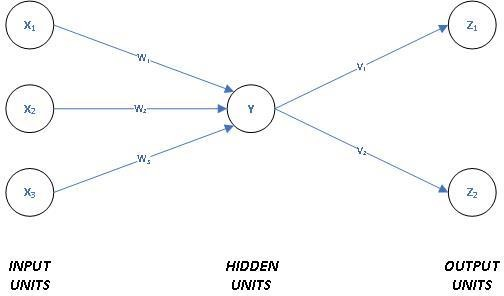
\includegraphics[width=0.5\textwidth]{Gambar/strukturdata}
	\caption{Struktur Dasar Jaringan Saraf Tiruan}
	\label{fig:g2}
\end{figure}

Pada \ref{fig:g2} dijelaskan bahwa setiap \textit{neuron} memiliki keadaan internal, yang disebut tingkat aktivasi atau aktivitas, yang merupakan fungsi dari input yang telah diterima. Biasanya, \textit{neuron} mengirimkan aktivasinya sebagai sinyal ke beberapa \textit{neuron} lain. Penting untuk dicatat bahwa \textit{neuron} hanya dapat mengirim satu sinyal pada satu waktu, meskipun sinyal itu disiarkan ke beberapa \textit{neuron} lain.

\section{Kohonen \textit{Self-Organizing Maps} (SOM)}

\textit{Self-Organizing Map} (SOM) pertama kali diperkenalkan oleh Teuvo Kohonen pada tahun 1982. SOM merupakan salah satu model dari Jaringan Saraf Tiruan. SOM merupakan salah satu tool untuk menangani data yang sangat besar, 
dimana data yang \textit{high-dimensional} data dapat divisualisasikan menjadi \textit{low-dimensional} data, atau mengurangi dimensi \textit{vector} \citep{Kohonen2013}.

Metode pembelajaran yang digunakan SOM adalah tanpa bimbingan dari suatu data \textit{input}-target atau \textit{unsupervised learning}. Artinya, sebuah jaringan akan belajar dengan dibekali pengetahuan dasar (parameter-parameter jaringan) tanpa adanya pengetahuan awal lebih dulu mengenai segmen dan karakteristiknya serta tanpa harus mengetahui berapa kelompok yang akan dibentuk, dan kemudian mengorganisasikan sendiri hubungan-hubungan interkoneksi dalam dirinya atas masukan yang diberikan sehingga dengan demikian target tidak dibutuhkan.

Di dalam SOM terdapat koneksi antara input-input dengan node-node yang memiliki bobot masing-masing. Sehingga, bobot yang telah ditentukan berkorespondensi untuk setiap node yang ada \citep{StefanovicKurasova2014a}. Himpunan bobot membentuk suatu vektor yang biasanya disebut neuron, dimana terdapat sejumlah baris dan kolom (dalam kasus ini, topologi yang diguanakn adalah topologi persegi panjang). Tujuan utama dari metode SOM ini adalah untuk mempertahankan topologi data multidimensi ketika mereka ditransformasikan menjadi ruang dimensi yang lebih rendah. Biasanya, metode SOM sendiri digunakan untuk mengelompokkan, mengklasifikasikan, dan memvisualisasikan berbagai jenis \textit{dataset}. SOM hanya dapat menangani data numerik, jadi pertama-tama, kita harus mengubah segala jenis dataset menjadi dataset     berekspresi     numerik.     Misalkan,     kita     memiliki    \textit{dataset} $X = \{ X_1, X_2, \ldots, X_n \}$, dimana     setiap     item     data     memiliki     beberapa     fitur $x_1, x_2, x_3, \ldots, x_n \ $ i.e. $\ X_i = \{ X_{i1}, X_{i2}, \ldots, X_{in} \}$.
Sehingga $X_i$ adalah vector dari $n$ ruang dimensi (\textit{n-dimensional data}), $X_i \in \mathbb{R}^n$. Semua \textit{dataset} dijadikan SOM sebagai matrix:

\[
\begin{bmatrix}
	X_{11} & X_{12} & \cdots & X_{1n} \\
	X_{21} & X_{22} & \cdots & X_{2n} \\
	\vdots & \vdots & \ddots & \vdots \\
	X_{N1} & X_{N2} & \cdots & X_{Nn}
\end{bmatrix}
\]

Berikut $X_{pl}$ merupakan nilai komponen dari vektor $X_i$, dimana $i = 1, 2, \ldots, N$, $l = 1, 2, \ldots, n$. 
Nilai $N$ merupakan jumlah vektor input yang dianalisis dan nilai $n$ merupakan jumlah komponen. 
Proses pembelajaran algoritme SOM dimulai dari inisialisasi komponen vektor (\textit{neuron}). 
Mereka dapat diinisialisasi secara acak (biasanya nilai-nilai ini adalah angka acak dari interval $(0, 1)$) 
atau oleh komponen utama $W_{ij}$. 
Pada setiap langkah pembelajaran, vektor masukan $X_i \in \{ X_1, X_2, \ldots, X_N \}$ dilewatkan ke SOM. 
Vektor $X_i$ dibandingkan dengan semua \textit{neuron} $W_{ij}$. 
Biasanya perhitungan bobot jarak menggunakan metode \textit{Euclidean Distance} antara vektor input $X_i$ 
dibandingkan dengan masing-masing neuron $W_{ij}$. 
Vektor (\textit{neuron}) $W_w$ dengan jarak \textit{Euclidean} minimal ke $X_i$ ditetapkan sebagai neuron pemenang 
(\textit{best match unit}) \citep{StefanovicKurasova2014a}. 
Semua komponen neuron diadaptasi sesuai dengan aturan pembelajaran berikut:

\[
W_{ij}(\text{new}) = W_{ij}(\text{old}) + h_w \big( X_i - W_{ij}(\text{old}) \big)
\]

\section{Arsitektur SOM}

Arsitektur SOM merupakan jaringan yang terdiri dari dua lapisan, yaitu lapisan \textit{input} dan \textit{output}.

\begin{figure}[h]
	\centering
	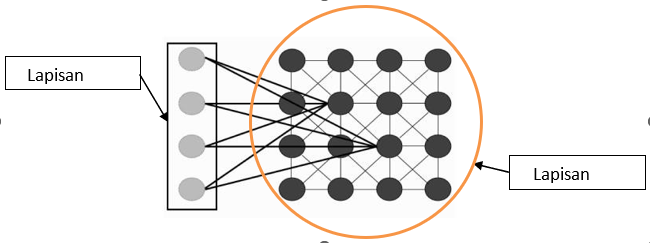
\includegraphics[width=0.8\textwidth]{Gambar/arsitektursom}
	\caption{Arsitektur SOM}
	\label{fig:g3}
\end{figure}

Pada \ref{fig:g3} dijelaskan bahwa setiap \textit{neuron} dalam lapisan \textit{input} terhubung dengan setiap \textit{neuron} pada lapisan \textit{output}. Setiap \textit{neuron} pada lapisan \textit{output} merepresentasikan kelompok dari \textit{input} yang diberikan.

\section{Parameter Pembelajaran (\textit{Learning Parameters})}

Hasil dari SOM bergantung pada parameter pembelajaran yang dipilih. Jadi, penting untuk memilih parameter pembelajaran yang terbaik dalam mendapatkan hasil yang terbaik dalam melakukan proses \textit{Clustering} data seperti ada penelitian ini. Hasil sebagian besar dipengaruhi oleh fungsi ketetanggaan (\textit{Neighboring Function}) dan \textit{learning rate} yang digunakan. Ada tiga fungsi ketetanggaan \textit{Bubble}, \textit{Gaussian} dan \textit{Heuristic} digunakan dalam proses pelatihan SOM \citep{StefanovicKurasova2014a}.

Pada penelitian ini, peneliti akan menggunakan fungsi ketetanggan \textit{Bubble} yang akan dipasangkan dengan \textit{learning rate} menggunakan \textit{Invers-of-time} untuk mendapatkan hasil \textit{Clustering} pada pelatihan SOM. Menurut \citep{StefanovicKurasova2014a}, penggunaan kombinasi tersebut untuk mendapatkan hasil yang terbaik dengan langkah perhitungan yang lebih sederhana, dengan tujuan mempercepat waktu proses kalkulasi pada sistem.

\section{Komponen penting SOM}

Menurut Simon Haykin terdapat tiga komponen penting dalam SOM yaitu:

\begin{enumerate}
	\item \textbf{\textit{Competition}}: Untuk setiap pola \textit{input}, neuron menghitung nilai masing-masing fungsi diskriminan yang memberi dasar untuk kompetisi.
	\item \textbf{\textit{Cooperation}}: Neuron pemenang menentukan lokasi spasial dari lingkungan topologi \textit{excited neuron} untuk memberi dasar kerjasama dalam suatu lingkungan \textit{neuron}.
	\item \textbf{\textit{Synaptic Adaption}}:\textit{ Excited neuron} menurunkan nilai fungsi diskriminan yang berkaitan dengan pola \textit{input} melalui penyesuaian bobot terkait sehingga respon dari \textit{neuron} pemenang keaplikasi berikutnya dengan pola \textit{input} yang sama akan meningkat.
\end{enumerate}

\section{Cara Kerja SOM}

Berikut   ini    merupakan    tahapan-tahapan    dalam    proses    \textit{Clustering} menggunakan SOM:

\begin{enumerate}
	\item Inisialisasi bobot ($W_{ij}$) yang diperoleh secara acak untuk setiap node. 
	Setelah bobot diberikan maka jaringan diberikan \textit{input} ($X_i$).
	
	\item Setelah input diterima, jaringan akan melakukan perhitungan jarak vektor $D(j)$ 
	yang didapat dengan menjumlahkan selisih antara vektor bobot dengan vektor \textit{input}:
	\[
	D_j = \sum_{k=0}^{i} (W_{ij} - X_i)^2
	\]
	
	\item Setelah jarak antara node diketahui maka ditentukan nilai minimum dari 
	perhitungan jarak vektor $D(j)$, maka tahap selanjutnya yaitu perubahan bobot:
	\[
	W_{ij}(\text{new}) = W_{ij}(\text{old}) + \alpha (x_i - W_{ij}(\text{old}))
	\]
	
	\item Pada proses untuk mendapatkan bobot baru diperlukan nilai \textit{learning rate} 
	($\alpha$) yaitu $0 \leq \alpha \leq 1$ dan untuk setiap \textit{epoch} akan mengalami penurunan 
	(\textit{decrease}) pada nilai \textit{learning rate} dengan cara 
	\[
	\alpha(i+1) = 0.5 \alpha
	\]
	
	\item Iterasi dihentikan ketika iterasi yang dilakukan sudah mencapai iterasi maksimum 
	yang ditentukan atau selisih antara $W_{ij}(\text{new})$ dengan $W_{ij}(\text{old})$ 
	hanya berubah sedikit saja, yang berarti hasil pengujian sudah dapat dikatakan 
	\textit{convergent}.
\end{enumerate}

\section{Teori Graf}

Berkembangnya ilmu pengetahuan dan teknologi secara pesat membuat matematika menjadi sangat penting artinya. Karena perkembangan ilmu pengetahuan dan teknologi tidak lepas dari peranan matematika. Hampir dapat dipastikan bahwa setiap bagian dari ilmu dan teknologi baik dalam unsur kajian  umum ilmu murni maupun terapannya memerlukan peranan matematika sebagai ilmu bantunya. Matematika digunakan sebagai alat penting di berbagai bidang, termasuk ilmu alam, teknik, kedokteran/medis, ilmu sosial seperti ekonomi, dan psikologi. Matematika terdiri dari beberapa cabang ilmu misalnya Aljabar, Geometri, Statistika, Probabilitas, Matematika Aplikasi, Matematika Komputasi, Matematika Ekonomi, Matematika Diskrit, Sain Komputer dan lain sebagainya. Cabang matematika terkini terkait dengan sain komputer yang cukup terkenal adalah teori graf. Teori graf merupakan teori lama yang hingga saat ini semakin banyak ditemukan aplikasinya di sekitar kita. Ide dasarnya diperkenalkan pertama kali pada abad ke-18 oleh matematikawan Swiss, Leonhard Euler. Pada waktu itu, ia menggunakan graf untuk menyelesaikan masalah jembatan Konigsberg. Teori graf merupakan pokok bahasan yang relatif muda namun memiliki banyak terapan yang sangat luas. Contohnya optimasi jaringan telepon, jaringan komputer, jaringan listrik, model papan sirkuit, model struktur ikatan kimia dan lain-lain. Graf digunakan dalam kehidupan sehari-hari untuk mendeskripsikan model persoalan dan menggambarkannya secara konkret dan jelas, mempresentasikan objek-objek diskrit dan hubungan antara objek tersebut. Inti dari cara pengaplikasian graf ini adalah bagaimana kita bisa membaca permasalahan, kemudian mendefinisikan apa yang akan menjadi objek diskrit yang kemudian akan menjadi simpul-simpul dari graf yang akan kita bangun untuk menggambarkan permasalahan yang kita hadapi tadi, apabila telah kita dapatkan simpul simpul maka akan mudah bagi kita untuk membangun graf dengan memberi sisi pada simpul-simpul yang saling berhubungan. Representasi visual dari graf adalah dengan menyatakan objek sebagai noktah, bulatan atau titik (verteks), sedangkan hubungan antara objek tersebut dinyatakan dengan garis atau sisi (\textit{edge}) \citep{Rahayuningsih2018}. Salah satu kajian yang menarik dalam graf adalah pelabelan graf. Sejak saat itu kajian mengenai pelabelan graf bermunculan dan berkembang pesat belakangan ini. Hingga saat ini pemanfaatan teori pelabelan graf sangat dirasakan peranannya, terutama pada sektor sistem komunikasi dan transportasi, navigasi geografis, radar, penyimpanan data komputer, dan pemancar frekuensi radio. Pelabelan pada suatu graf adalah suatu pemetaan (fungsi) yang memasangkan unsur-unsur graf (titik dan/atau sisi) dengan bilangan (biasanya bilangan bulat). Jika domain dari fungsi adalah titik, maka pelabelan tersebut dinamakan pelabelan titik (\textit{vertex labellings}), jika domainnya adalah sisi, maka pelabelannya disebut pelabelan sisi (\textit{edge labellings}) dan jika domainnya adalah titik dan sisi, maka pelabelannya disebut pelabelan total (total labellings). Hingga kini dikenal beberapa jenis pelabelan pada graf, antara lain pelabelan \textit{graceful} (\textit{graceful labeling}), pelabelan harmoni (\textit{harmonious labeling}), pelabelan total tak beraturan (\textit{total irregularity labeling}), pelabelan ajaib (\textit{magictype labeling}), dan pelabelan anti ajaib (\textit{antimagic-type labeling}). Pelabelan total titik \textit{irregular} merupakan pemberian nilai bilangan bulat positif (nilai yang dipakai boleh berulang) pada himpunan titik dan sisi dari suatu graf G, dengan bobot. setiap sisinya berbeda. Untuk sebuah graf G terdapat beberapa variasi pelabelan total sisi \textit{irregular}, dengan kata lain pelabelannya tidak tunggal. Dalam pelabelan graf ini, asalkan bobot setiap sisinya berbeda maka pelabelan tersebut dinamakan dengan pelabelan total sisi \textit{irregular}. Permasalahannya adalah bagaimana melabeli graf tersebut sedemikian hingga bilangan bulat positif terbesar yang di   jadikan   label   pada   beberapa   variasi   pelabelan total sisi \textit{irregular} adalah seminimum mungkin. Bilangan bulat positif terbesar yang minimum tersebut dinamakan dengan \textit{total irregularity edge strength} dari graf G yang dinotasikan dengan \textit{tes}(G). Salah satu algoritma graf adalah Pohon Rentang (\textit{Spanning Tree}) pada suatu \textit{graph} adalah \textit{subgraph} minimal yang menghubungkan semua simpul pada \textit{graph}. Apabila graf tersebut adalah graf berbobot (\textit{Weighted Graph}), kemudian dari pohon rentang yang dimiliki oleh graf didefinisikan sebagai penjumlahan dari bobot–bobot seluruh cabang pada pohon rentang maka akan diperoleh pohon rentang yang memiliki bobot. Pohon rentang yang memiliki bobot terkecil pada suatu graf berbobot disebut Pohon rentang Minimum (\textit{Minimum spanning tree}). Salah satu contoh optimasi jaringan menjadikan adanya kebutuhan untuk mencari nilai terkecil (minimal) pada suatu keadaan jaringan. Salah satu masalah optimasi jaringan adalah \textit{Minimum spanning tree} (MST), yaitu suatu keadaan dimana semua \textit{node} dalam graf terhubung, namun tidak boleh terdapat \textit{loop} didalamnya dan dihitung bobot \textit{tree} yang terkecil. Salah satu aplikasi MST adalah pembuatan jaringan komunikasi atau telepon yang akan menghubungkan semua stasiun telepon pada suatu kota yang ada. Permasalahannya adalah mencari jarak terpendek antara kota-kota tersebut sehingga penggunaan kabel akan lebih sedikit yang berarti menghemat biaya pembangunan jaringan telepon tersebut \citep{Afrianto2012}. 

\textbf{Pohon $m$-\textit{ary}} adalah pohon berakar yang setiap simpul cabangnya mempunyai paling banyak $m$ buah anak. 
Jika $m = 2$, pohonnya disebut \textbf{pohon \textit{biner (binary tree)}}. 
Pohon $m$-\textit{ary} dikatakan \textbf{teratur} atau penuh\textbf{penuh} (\textit{full}) jika setiap simpul cabangnya mempunyai tepat $m$ anak.

\begin{figure}[h]
	\centering
	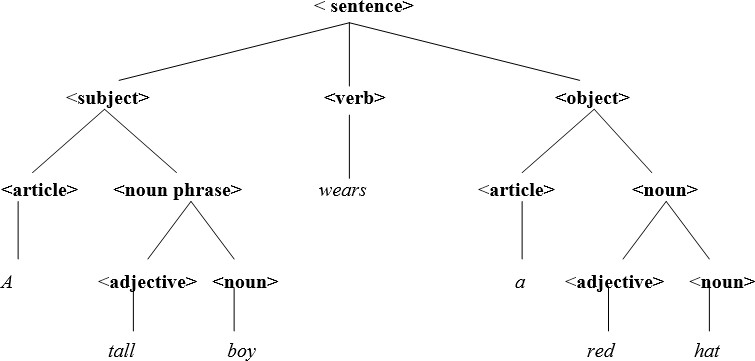
\includegraphics[width=0.8\textwidth]{Gambar/pohonparsing}
	\caption{Pohon \textit{parsing} dari kalimat \textit{A tall boy wears a red hat}}
	\label{fig:g4}
\end{figure}

\section{Validasi Kelompok}

Dalam proses \textit{Clustering}, validasi sistem sudah menjadi sebuah bagian cukup krusial dalam proses membangun model \textit{Clustering}, ukuran dan metode untuk mengevaluasi. Model dibangun menggunakan set data latih dengan sejumlah parameter yang diminta oleh metode yang digunakan. Dalam analisis kelompok, evaluasi dilakukan dengan melakukan pemrosesan data secara alami dengan algoritme yang berjalan sendiri sehingga didapatkan kelompok-kelompok yang terbentuk secara alami pula.

Nilai validasi sangat bermanfaat guna membandingkan apakah algoritme yang digunakan pada penelitian ini menghasilkan tingkat akurasi yang lebih baik dari penelitian-peneliatan sebelumnya yang menggunakan metode selain \textit{Self Organizing Maps} (SOM) yang digunakan untuk \textit{Clustering} suatu data. Pada penelitian ini nilai validasi digunakan apakah dengan menggunakan metode SOM saja sudah cukup menghasilkan tingkat akurasi yang baik atau tidak. Proses validasi dilakukan dengan cara melatih data dan membandingkan kesesuaian hasil \textit{Clustering} data. Validasi kelompok yang digunakan dalam penelitian ini menggunakan \textit{Davies-Bouldin Index} \citep{Dan2015}.

Indeks \textit{silhouette} dan \textit{Davies-Bouldin} adalah dua metode yang digunakan dalam pembelajaran mesin untuk mengevaluasi kualitas kelompok. Indeks \textit{silhouette} digunakan untuk mengevaluasi seberapa baik setiap titik data tergabung dalam kelompok yang sesuai. Ini dilakukan dengan menghitung jarak antara setiap titik data dan kelompok lain yang berdekatan, lalu membandingkannya dengan jarak antara titik data tersebut dan kelompok tempat ia tergabung. Nilai \textit{silhouette} yang lebih tinggi menunjukkan bahwa titik data tersebut lebih baik tergabung dalam \textit{cluster} tempat ia berada. \textit{Davies-Bouldin Index}, di sisi lain, mengevaluasi seberapa baik \textit{cluster-cluster} dipisahkan satu sama lain. Ini dilakukan dengan menghitung rata-rata jarak antara setiap \textit{cluster} dan \textit{cluster} lain yang berdekatan. Nilai yang lebih rendah menunjukkan bahwa \textit{cluster-cluster} lebih baik dipisahkan satu sama lain. Kedua metode ini bertujuan untuk mengevaluasi kualitas \textit{clustering} dan membantu dalam membuat keputusan tentang apakah \textit{clustering} yang dilakukan menghasilkan hasil yang baik atau tidak \citep{Dan2015}.

\section{\textit{Davies-Bouldin Index}}

Validasi kelompok \textit{Davies-Bouldin Index} (DBI) diperkenalkan oleh David L. Davies dan Donald W. Bouldin pada tahun 1979 yang digunakan untuk mengevaluasi kelompok. Validasi internal yang dilakukannya adalah seberapa baik \textit{Clustering} sudah dilakukan dengan menghitung kuantitas dan fitur turunan dari set data.
\textit{Sum of square within cluster} (SSW) dalam sebuah kelompok diformulasikan sebagai berikut: 

\[
SSW_i = \frac{1}{m} \sum_{j=1}^{m_i} d(x_j, c_i)
\]

dengan $mi$ adalah jumlah data yang berada dalam  kelompok ke-$i$, sedangkan $ci$
adalah centroid kelompok ke-$i$.

\textit{Sum of square between cluster} (SSB) dengan mengukur jarak dua kelompok, misalnya kelompok-$i$ dan kelompok-$j$, dengan formula mengukur jarak antara centroid
$ci$ dan $cj$ pada persamaan berikut:

\[
SSB = d(c_i, c_j)
\]

Didefinisikan $R_{ij}$ adalah ukuran rasio seberapa baik nilai perbandingan antara kelompok ke-$i$ dan kelompok ke-$j$. Nilainya didapatkan dari komponen SSW dan SSB. Kelompok yang baik adalah kelompok yang memiliki SSW sekecil mungkin dan SSB yang sebesar mungkin. $R_{ij}$ diformulasikan dengan persamaan berikut:

\[
R_{ij} = \frac{{SSW}_i + {SSW}_j}{{SSB}_{ij}}
\]

Sifat-sifat yang dimiliki $R_{ij}$ sebagai berikut:

\begin{enumerate}
	\item $R_{i,j} \ge 0$
	\item $R_{i,j} = R_{j,i}$
	\item Jika $SSW_j \ge SSW_r$ dan $SSB_{i,j} = SSB_{i,r}$ maka $R_{i,j} > R_{i,r}$
	\item Jika $SSW_j = SSW_r$ dan $SSB_{i,j} \le SSB_{i,r}$ maka $R_{i,j} > R_{i,r}$
\end{enumerate}

Nilai \textit{Davies-Bouldin Index} (DBI) didapatkan dari persamaan berikut: 

\[
DBI = \frac{1}{K} \sum_{i=1}^{K} \max_{j \ne i} (R_{i,j})
\]

$K =$ jumlah kelompok yang digunakan.

Secara esensial, DBI menginginkan nilai sekecil mungkin yang bisa dihasilkan (non-negatif $\geq 0$) untuk menilai baiknya kelompok yang didapat. Nilai yang didapat bisa digunakan sebagai pendukung keputusan untuk menilai jumlah kelompok yang paling cocok digunakan \citep{Dan2015}.

\section{\textit{Silhoutte Coeffisient}}

Pengujian yang dilakukan menggunakan \textit{Silhoutte Coeffisient}. Metode ini berfungsi untuk menguji kualitas dari kelompok yang terbentuk dari hasil metode SOM-MST.
Menurut Romdhoni \citep{Kmeans2018} terdapat 3 langkah yang dilakukan untuk menghitung \textit{Silhoutte Coeffisient} yaitu:

\begin{enumerate}
	\item Hitung rata-rata jarak dari objek $i$ terhadap seluruh objek yang berada dalam satu kelompok.
	\item Hitung rata-rata jarak dari objek $i$ terhadap seluruh objek yang berada pada kelompok lainnya.
	\item Nilai \textit{Silhouette Coefficient} dari objek $i$ menggunakan Persamaan \ref{eq:1}:
	
	\begin{equation}\label{eq:1}
		S_i = \frac{b_i - a_i}{\max(b_i, a_i)}
	\end{equation}
	Dimana:
	\begin{itemize}
		\item $S_i$ = \textit{Silhouette Coefficient} dari objek $i$
		\item $a_i$ = Rata-rata jarak objek $i$ terhadap seluruh objek di dalam kelompok
		\item $b_i$ = Rata-rata jarak objek $i$ terhadap seluruh objek di luar kelompok
	\end{itemize}
	Ukuran nilai \textit{Silhouette Coefficient} \citep{Gentle1991}:
	\begin{enumerate}
		\item $0.7 < SC \le 1$ menyatakan struktur kuat
		\item $0.5 < SC \le 0.7$ menyatakan struktur sedang
		\item $0.25 < SC \le 0.5$ menyatakan struktur lemah
		\item $SC \le 0.25$ menyatakan tidak ada struktur
	\end{enumerate}
\end{enumerate}


\chapter{KERANGKA KONSEPTUAL PENELITIAN}

\section{Permasalahan dan Tantangan Penelitian}

Dalam pengertian yang sangat luas, orang biasa mengenal data mining dengan pengolahan data dengan berbagai macam teknik dengan ukuran data yang beragam. Data \textit{mining} sebagai bidang yang menggabungkan bidang‐bidang keilmuan terkait seperti pengenalan pola, \textit{database}, \textit{machine learning}, statistik, serta  visualisasi guna menangani masalah-masalah dalam mengambil suatu informasi dari banyaknya data yang ada. Data mining merupakan suatu proses yang memanfaatkan \textit{artificial intelligence}, teknik statistik, \textit{machine learning}, dan juga matematika guna melakukan identifikasi dan ekstraksi informasi serta suatu pengetahuan yang sekiranya akan bermanfaat dari berbagai database yang berukuran besar (Decision Support Systems and Intelligent Systems 7th Edition (PDFDrive).Turban, 2015)

\textit{Clustering} adalah salah satu metode data mining dimana sekelompok data akan dibagi ke dalam beberapa kelompok yang terbentuk secara alami berdasarkan  kesamaan karakteristik  data  masing-masing  dalam sebuah  dataset yang besar \citep{Singh2011}. Terkait dengan penelitian ini, terdapat penelitian‐penelitian     yang telah  dilakukan  sebelumnya, baik tentang media pembelajaran digital maupun tentang algoritma yang digunakan, yakni \textit{Self‐Organizing Map} (SOM) dan juga kombinasinya dengan m-aT. Penelitian-penelitian terdahulu ini digunakan sebagai landasan dalam proses penelitian.

Pada tahun 2019, sebuah penelitian tentang memetakan siswa berdasarkan aktivitasnya di media pembelajaran digital pernah dilakukan secara manual. Dalam penelitian ini, analisis dilakukan secara manual dengan mengambil kesimpulan melalui visualisasi dan persepsi peneliti. Siswa dipetakan menjadi empat kelompok berdasarkan pola siswa dalam menyelesaikan permasalahan dalam Monsakun. Hasil pemetaan dapat mengatakan bahwa siswa disetiap kelompok membutuhkan perlakuan yang berbeda-beda \citep{SupiantoHayashiHirashima2019}.

Sebuah penelitian dengan adaptasi lebih lanjut dari pemetaan performa belajar siswa juga telah dilakukan. Penelitian ini dilakukan untuk mengelompokan siswa pengguna \textit{E-Learning} secara otomatis dengan menggunakan algoritme SOM. Data yang digunakan dalam penelitian ini merupakan sekumpulan data interaksi dan aktivitas siswa yang mengambil mata pelajaran  Algoritme dan  Struktur Data ketika  menggunakan \textit{E‐Learning}. Pada penelitian ini, atribut yang digunakan dipilih menggunakan \textit{Principal Component Analysis} (PCA) terlebih dahulu sebelum kemudian diproses dengan SOM. Kemudian melalui proses tersebut, dihasilkan \textit{Low Browsing cluster} dan \textit{High Browsing cluster}. Adapun pengujian yang dilakukan dalam penelitian ini dengan menggunakan \textit{Silhouette index}, \textit{Dunn index}, dan \textit{Davies-Bouldin index} dan membandingkannya dengan K-Means dan \textit{Partitioning Around Medoids} dan memunculkan SOM sebagai algoritma yang cukup baik untuk melakukan \textit{Clustering} terhadap log data aktivitas siswa karena memiliki hasil terbaik pada nilai Silhouette index sebesar $0.4502$ dan \textit{Dunn index} sebesar $1.1452$ \citep{Alias2017}.

Selain digunakan dalam bidang pendidikan, SOM juga banyak digunakan dalam  bidang-bidang  lainnya. Salah  satunya  adalah  penelitian  yang  dilakukan oleh Dini dan \citet{Dini2020}, bahwa hasil \textit{Clustering} 34 provinsi di Indonesia dengan indikator kesejahteraan masyarakat yang terdiri dari enam indikator diperoleh metode terbaik dengan menggunakan analisis \textit{cluster K-Means}. Analisis \textit{cluster K-Means} dipilih karena didasarkan pada nilai varians $(0,101)$ yang lebih kecil dari nilai varians Average Linkage Clustering $(0,152)$. Selain itu, diketahui bahwa kesejahteraan masyarakat di Indonesia Indonesia masih belum merata. Hal ini dapat dilihat pada karakteristik masing-masing \textit{cluster}. Setiap kelompok memiliki prioritas yang berbeda dalam yang berbeda dalam bidang kesejahteraan yang perlu diperhatikan atau ditingkatkan oleh pihak-pihak terkait. Provinsi-provinsi yang berada di kelompok pertama dapat menjadi prioritas dalam berbagai aspek kesejahteraan bagi pemerintah agar kesejahteraan dapat dirasakan secara adil oleh masyarakat. Kesejahteraan dapat dirasakan secara adil oleh masyarakat. Sementara itu, provinsi yang berada di kelompok kedua dan ketiga masih perlu mendapat perhatian dalam beberapa aspek kesejahteraan masyarakat. Visualisasi kelompok dalam bentuk peta Indonesia diharapkan dapat memudahkan untuk menggambarkan kondisi umum kesejahteraan provinsi-provinsi di Indonesia \citep{Dini2020}.

Tak hanya itu, SOM juga digunakan pada penelitian lain di berbagai bidang sesuai  keahlian  masing-masing  peneliti.  Seperti  penelitian  yang  dilakukan  oleh \citet{Oliver2018} di bidang biologi, atau penelitian yang dilakukan oleh \citet{Pisano2017} dan \citet{MolinaGarcia2019} di bidang kesehatan. Penelitian-penelitian  ini membuktikan bahwa algoritme SOM tidak hanya dapat digunakan untuk bidang tertentu seperti pendidikan saja, melainkan dapat digunakan pula untuk bidang-bidang lainnya.
Penelitian  lain  yang  juga  menjadi  acuan  penelitian  ini  adalah  penelitian-penelitian yang menggunakan pengembangan dari algoritme SOM konvensional dalam prosesnya. Salah satunya adalah penelitian yang bergerak di bidang Biologi dengan menggunakan dua jenis dataset, yakni \textit{Human Fibroblasts Serum} (HFS) dataset dan Rat CNS dataset. Kedua data kemudian diolah dan divisualisasikan dengan menggunakan algoritme SOM. Map size yang dihasilkan pada HFS cukup beragam, yakni $6×2$, $4×3$, dan $3×4$. Sementara CNS mengeluarkan ukuran yang sama, yakni 3×3. Setelah data selesai diolah, data diuji dengan menggunakan Silhouette index. Hasil pengujian dalam penelitian ini menunjukkan nilai \textit{Silhouette} sebesar lebih dari 0.6 untuk setiap data HFS, dan $0.5927942$ untuk seluruh data CNS. Selanjutnya algoritme SOM yang telah dikembangkan dalam penelitian ini disebut dengan SOMHS \citep{George2015}. 

Mayoritas pengembangan dari SOM konvensional hanya bisa digunakan pada kasus tertentu saja. Namun, sebuah penelitian lain yang juga merupakan pengembangan dari SOM berhasil dilakukan pada tahun 2019. Penelitian ini membahas mengenai kombinasi dari penggunaan \textit{Self Organizing Map} (SOM) dan \textit{Fuzzy C-Means} (FCM) dalam \textit{Clustering} yang bertujuan untuk mengevaluasi kualitas air tanah di Seoul, Korea Selatan. Penelitian tersebut  mengatakan bahwa SOM dan FCM yang sama-sama mampu diterapkan dalam sekumpulan data besar yang kompleks akan saling melengkapi jika dikombinasikan. Hal ini terjadi karena baik SOM dan FCM sama-sama memiliki kekurangan dan saling membutuhkan. SOM yang dikenal dengan visualisasinya seringkali memunculkan ambiguitas pada keluarannya hingga FCM dirasa  cocok untuk  membantu  menciptakan batasan-batasan  kelompok  dari  hasil keluaran SOM tersebut. Kedua algoritme ini juga mudah diterapkan sehingga dapat  diimplementasikan tidak hanya pada kasus-kasus  tertentu \citep{Lee2019}.

Penambangan atau eksplorasi data adalah bagian dari area penelitian terbaru  yang lebih luas dalam Kecerdasan Buatan dan Pemrosesan dan Manajemen Informasi atau dikenal sebagai \textit{Knowledge Discovery in Database} (KDD). Tujuannya untuk mengidentifikasi informasi atau pengetahuan baru dari database di mana dimensi atau jumlah data sangat besar sehingga melampaui pemahaman manusia. MST digunakan untuk menganalisis basis data transformator daya dari satu dari penyedia energi listrik di Jepang. Evaluasi kelompok dihasilkan oleh SOM biasanya dilakukan oleh mata manusia. Karena sifatnya kualitatif alam, evaluator dapat melebih-lebihkan atau meremehkan jumlah kelompok yang terbentuk di peta. Dengan pendekatan ini, tepat jumlah kelompok yang dihasilkan oleh peta tidak dapat dikonfirmasi karena salah tafsir dari ekspresi tingkat abu-abu (Tokutaka et al., 2001).
Penelitian tentang teknik visualisasi menggunakan SOM dan MST. Metode ini dapat mengungkapkan kelompok barang serupa, berdasarkan graf yang dibangun baik dari data input, atau node SOM. Evaluasi visualisasi, dan membandingkannya dengan metode graf kerapatan, dan menemukannya untuk mengungkapkan informasi serupa. Visualisasi tidak bergantung pada parameter pengguna tertentu, yang bermanfaat bagi pengguna pemula. Metode operasi pada simpul SOM umumnya memiliki waktu komputasi yang lebih rendah daripada metode graf kepadatan, karena jumlah node dalam SOM umumnya besarnya lebih kecil dari jumlah sampel data \citep{MayerRauber2010}.

Penelitian algoritma SOM-MST yang menggabungkan SOM dengan graf MST dan membahas bagaimana MST dari sebuah graf yang mencapai subset sisi yang paling ekonomis yang menghubungkan semua komponen dengan sebuah \textit{loop} terbuka. Dalam penelitian ini, MST pada SOM dengan sub-simpul yang disematkan dan ukuran jarak untuk pilihan ukuran dan bentuk peta yang optimal. Penelitian ini mendemonstrasikan dengan menggunakan data \textit{Fisher's Iris} dan data ekspresi gen yang nyata. Kumpulan data simulasi juga dianalisis untuk memeriksa validitas metode yang diusulkan (Jang et al., 2009).

Penelitian yang terkait dengan kombinasi SOM dan teori graf adalah SOM graf teoretis ke domain data hierarkis. Hasilnya memiliki kompleksitas algoritmik yang lebih rendah daripada SOM asli,dan dapat menghasilkan SOM yang memiliki validitas kelompok yang jauh lebih tinggi daripada pengkodean biner \citep{Argyrou2009}, menggunakan pemetaan probabilitas selama \textit{Graph}-SOM \citep{Hagenbuchner2009}, pelatihan \textit{Graph}-MST-SOM membantu meningkatkan kinerjanya secara signifikan dan membantu secara substansial mengurangi permintaan komputasi \citep{MayerRauber2010,Resta2016} dan hasilnya mendukung penggunaan pendekatan teoretis graf seperti dalam semua eksperimen jumlah kelompok yang ditemukan sudah benar dan valid \citep{Silva2011}.

Heba Mohmmed Nagy Rashad, 2013, meneliti tentang Penambangan data pendidikan adalah bidang penambangan data tertentu diterapkan pada data yang berasal dari lingkungan pendidikan, bergantung pada pendekatan yang berbeda untuk menemukan pengetahuan yang tersembunyi dari data yang tersedia. Di antara pendekatan tersebut adalah teknik pembelajaran mesin yang digunakan untuk membangun sistem yang memperoleh pengetahuan tersembunyi dari data sebelumnya. Pembelajaran mesin dapat diterapkan untuk memecahkan masalah yang berbeda regresi, klasifikasi, \textit{Clustering} dan optimasi masalah. 

Dalam penelitian ini mengusulkan “Penasehat Siswa” yang adapun permasalahan dan tantangan dalam penelitian ini untuk menerapkan kombinasi dari algoritme SOM dan m-aT di bidang penambangan data Monsakun sebagai data pendidikan. Data yang digunakan dalam penelitian ini merupakan log data yang dihasilkan melalui rekaman aktivitas belajar belajar siswa pada media pembelajaran digital bernama Monsakun. Selanjutnya melalui sebuah proses pengolahan, data tersebut akan menghasilkan \textit{Clustering} siswa dan sistem penasehat guru yang dapat digunakan untuk \textit{Clustering} performa belajar siswa agar umpan balik siswa ke guru atau sebaliknya yang tepat dapat diberikan sebagai dasar melakukan evaluasi pembelajaran problem posing integrasi kalimat  cerita aritmatika.

\section{Ide Umum Penelitian}
Ide umum penelitian ini adalah:
\begin{enumerate}
	\item Untuk membuat analisis proses \textit{Clustering} siswa.
	\item Untuk penasehat pembelajaran oleh guru dalam problem posing melalui integrasi kalimat Cerita Aritmatika menggunakan \textit{Self-Organizing Map-m-Ary Tree} (SOM-m-aT).
	\item Persepsi guru Sekolah Dasar di Indonesia tentang sistem penasehat pembelajaran berdasarkan kemiripan siswa.
\end{enumerate}

\begin{figure}[h]
	\centering
	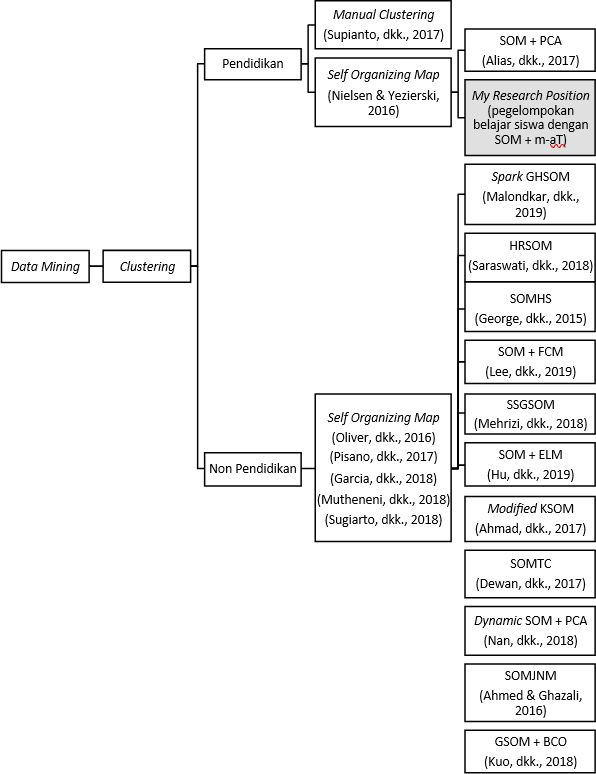
\includegraphics[width=0.5\textwidth]{Gambar/bagankerangka}
	\caption{Bagan kerangka konseptual penelitian}
	\label{fig:g5}
\end{figure}

\begin{landscape}
	\begin{center}
		\renewcommand{\arraystretch}{1.2}
		\setlength\extrarowheight{2pt}
		
		\begin{tabularx}{\linewidth}{|Y|Y|c|Y|Y|Y|}
			\caption{Matriks pemetaan posisi penelitian untuk metode penelitian dengan SOM dan Graf} \label{tab:1} \\
		
			\hline
			\textbf{Nama Peneliti} & \textbf{Judul Paper} & \textbf{SOM} & \textbf{Graf} & \textbf{Dataset} & \textbf{Jenis Paper} \\
			\hline
			\endfirsthead
			
			\hline
			\textbf{Nama Peneliti} & \textbf{Judul Paper} & \textbf{SOM} & \textbf{Graf} & \textbf{Dataset} & \textbf{Jenis Paper} \\
			\hline
			\endhead
			
			Argyris Argyrou, 2009 & \textit{Clustering Hierarchical Data Using Self-Organizing Map: A Graph-Theoretical Approach}
			& $\checkmark$ & teori graf & the zoo-dataset [9] berisi 101 binatang & Prosiding \\ \hline
			
			Markus Hagenbuchner, dkk., 2009 & \textit{Projection of undirected and non-positional graphs using Self Organizing Maps}
			& - & \textit{Probabilitas mapping Graph SOM (PM-Graph-SOM).} & Terdiri dari 114, 366 yang melalui hyperlinks. & Prosiding \\ \hline
			
			Rudolf Mayer dan Andreas Rauber, 2010 & \textit{Visualising Clusters in Self-Organising Maps with Minimum Spanning Trees}
			& - & MST & Iris & Prosiding \\ \hline
			
			Leandro A. Silva dan José Alfredo F. Costa, 2011 & \textit{A Graph Partitioning Approach to SOM Clustering}
			& - & \textit{Graph Partitioning Approach} & \textit{Synthetic, Spiral, Iris-database} & Prosiding \\ \hline
			
			Marina Resta, 2012 & \textit{Graph Mining Based SOM: A Tool to Analyze Economic Stability}
			& - & MST & Ekonomi & Book Chapter \\ \hline
			
			Marina Resta, 2015 & \textit{Enhancing Self-Organizing Map Capabilities with Graph Clustering : An Application to Financial Markets}
			& - & MST & Keuangan & Prosiding \\ \hline
			
			Supianto, A.A., dkk., 2016 & \textit{Visualizations of problem-posing activity sequences toward modeling the thinking process.}
			& - & - & $\checkmark$ Monsakun Data & Jurnal \\ \hline
			
			Supianto, A.A., dkk., 2017 & \textit{Model-based analysis of thinking in problem posing a sentence integration focused on violation of the constraints}
			& - & - & $\checkmark$ Monsakun Data & Jurnal \\ \hline
			
			Puteri Nor Ellyza Nohuddin, dkk., 2018 & \textit{Monitoring Students Performance using Self Organizing Map Trend Clustering}
			& - & - & - & Jurnal \\ \hline
			
			Musa Wakil Bara, dkk., 2018 & \textit{Self-Organizing Map Clustering Method for the Analysis of E-Learning Activities}
			& - & - & UTM Moodle LMS log records. & Prosiding \\ \hline
			
			Abla Chaouni Benabdellah, dkk., 2019 & \textit{A survey of clustering algorithms for an industrial context}
			& - & - & Logistik, kebutuhan Pelanggan, Sistem kualitas Otomotif dan Pesawat & Prosiding \\ \hline
			
			Fitri Latifah, 2016 & \textit{Penerapan Algorithma Pohon untuk Operasi Pengolahan dan Penyimpanan Data dalam Teknik Pemrograman}
			& - & $\checkmark$ \textit{m-ary-tree} & Data Teknik Pemrograman & Jurnal \\ \hline
			
			César A. Astudillo dan B. John Oommen, 2009 & \textit{On Using Adaptive Binary Search Trees to Enhance Self Organizing Maps}
			& - & Graf pohon (BST) & TTO-CONROT dataset & Prosiding \\ \hline
			
			Nabila Divanadia Luckyana, dkk., 2021 & \textit{Implementasi Kombinasi Algoritme Self-Organizing Map dan Fuzzy C-Means untuk Clustering Performa Belajar Siswa pada Media Pembelajaran Digital}
			& - & - & $\checkmark$ Data Monsakun & Prosiding \\ \hline
			
			Tibyani, dkk, 2022 & - & - & $\checkmark$ \textit{m-ary-tree} & $\checkmark$ Data Monsakun & Jurnal dan Prosiding \\ \hline
			
		\end{tabularx}
	\end{center}
\end{landscape}


\begin{landscape}
	\begin{table}
		\centering
		\renewcommand{\arraystretch}{1.2}
		\setlength\extrarowheight{2pt}
		\caption{Matriks pemetaan posisi penelitian untuk metode penelitian sistem penasehat oleh guru atau dosen}
		\label{tab:2}
		\begin{tabularx}{\linewidth}{|Y|Y|c|Y|c|}
			\hline
			\textbf{Nama Peneliti} & \textbf{Judul} & \textbf{Teknologi} & \textbf{Dataset} & \textbf{Jenis Paper} \\
			\hline
			Heba Mohmmed Nagy Rashad, 2013 & \textit{Automated Student Advisory using Machine Learning} & Web & Institut Tinggi Kairo untuk Teknik, Ilmu Komputer, dan Manajemen menggunakan data yang dikumpulkan selama 12 tahun (2000–2012) & Jurnal \\
			\hline
			Olawande Daramola, dkk., 2014 & \textit{Implementation of an Intelligent Course Advisory Expert System} & $\checkmark$ & Dari Department of Computer and Information Sciences of Covenant University Nigeria & Jurnal \\
			\hline
			Ikono Rhoda Nsikan-Abasi, dkk., 2016 & \textit{Engineering of a Student Advisory Management System: Development Perspective} & $\checkmark$ & 24 Penasehat dari tujuh (7) fakultas Universitas Obafemi Awolowo, Nigeria. 120 siswa dipilih secara acak dari masing-masing fakultas & Jurnal \\
			\hline
			Tawafak, R.M., dkk., 2020 & \textit{A Review Paper on Student-Graduate Advisory Expert System} & – & Databases \textit{IEEE, Scopus, ScienceDirect, E-database}, dan \textit{ResearchGate} dengan total artikel 107,932 & Prosiding \\
			\hline
			Bamo Nadir Faraj dan Aree Ali Muhammed, 2021 & Online Course Registration and Advisory Systems Based on Students’ Personal and Social Constraints & $\checkmark$ & Data dari Komar University of Science and Technology (KUST), Irak & Jurnal \\
			\hline
		\end{tabularx}
	\end{table}
\end{landscape}

\chapter{METODE PENELITIAN}

\section{Tahapan Penelitian}

Secara garis besar, tahapan untuk melakukan penelitian ini dibagi menjadi:

\begin{enumerate}
    \item \textbf{Tahap persiapan}: Identifikasi dan perumusan masalah.
    \item \textbf{Tahap pengumpulan dan pengolahan data}.
    \item \textbf{Tahap analisis dan pembahasan}.
    \item \textbf{Kesimpulan}.
\end{enumerate}

Tahapan-tahapan yang dilakukan pada penelitian ini digambarkan pada Gambar.

\begin{enumerate}
    \item \textbf{Tahap Identifikasi dan Perumusan Masalah}

        \setlength{\parindent}{1cm}

        Pada tahap ini, konsep proposal yang telah disusun direview kembali, terutama yang terkait dengan kajian literatur dan metodologi. Hal ini dilakukan untuk memastikan bahwa hasil kajian teori yang digunakan cukup kuat sebagai dasar argumentasi atau pijakan dalam penelitian ini. Selain itu, juga dimaksudkan agar metodologi yang akan dipakai dapat diimplementasikan dalam penelitian ini.

        Tahapan identifikasi masalah dilakukan untuk mengidentifikasi permasalahan yang akan diteliti. Melalui studi literatur ditemukan bahwa perlunya dilakukan penyesuaian komponen pembelajaran ataupun metode pembelajaran bagi pelajar berdasarkan perilaku dan tingkat pengetahuan mereka \citep{Ahmad2015}. 

    \item \textbf{Tahap Pengumpulan dan Pengolahan Data}

        Data yang digunakan pada penelitian ini berupa data log aktivitas yang dikumpulkan dari aktivitas belajar siswa sekolah dasar di Jepang berusia 6 tahun pada sistem media pembelajaran \textit{MONSAKUN}. \textit{MONSAKUN} dirancang sebagai media pembelajaran interaktif untuk \textit{problem-posing} berdasarkan model \textit{triplet structure} \citep{Hirashima2014}. 

        Pemilihan data digunakan untuk melakukan seleksi dari kumpulan data menjadi data yang hanya sesuai dengan kebutuhan penelitian. Pada penelitian ini digunakan hanya data log aktivitas level 5 dari sistem pembelajaran \textit{MONSAKUN}. Hal ini dikarenakan rata-rata langkah dan kesalahan pada level 5 jauh lebih tinggi jika dibandingkan dengan level 1 hingga level 4, sehingga dapat dikatakan bahwa level 5 lebih menantang jika dibandingkan level lainnya (Supianto, et al., 2016).

        Pengolahan data dilakukan untuk merubah bentuk data menjadi bentuk yang dibutuhkan dalam penelitian. Pada tahapan ini data log aktivitas pelajar yang masih berbentuk data sequence diubah menjadi data dengan fitur-fitur yang sesuai dengan kebutuhan penelitian. Fitur-fitur dari data yang digunakan pada penelitian ini berupa:

        \begin{enumerate}
            \renewcommand{\labelenumii}{\arabic{enumii}.}
            \item Id pelajar: Berisi variabel \textit{primary key} yang membedakan tiap-tiap pelajar.
            \item Lama: Berisi waktu pengerjaan tugas oleh pelajar dalam satuan detik.
            \item Langkah: Berisi jumlah langkah (\textit{set} dan \textit{remove}) yang dilakukan pelajar.
            \item \textit{Set}: Berisi jumlah langkah \textit{set} yang dilakukan pelajar.
            \item \textit{Remove}: Berisi jumlah langkah \textit{remove} yang dilakukan pelajar.
            \item C1: Berisi jumlah penggunaan kartu 1 oleh pelajar.
            \item C2: Berisi jumlah penggunaan kartu 2 oleh pelajar.
            \item C3: Berisi jumlah penggunaan kartu 3 oleh pelajar.
            \item C4: Berisi jumlah penggunaan kartu 4 oleh pelajar.
            \item C5: Berisi jumlah penggunaan kartu 5 oleh pelajar.
            \item C6: Berisi jumlah penggunaan kartu 6 oleh pelajar.
            \item \textit{Unique}: Berisi jumlah susunan kartu unik yang digunakan pelajar.
            \item \textit{Error}: Berisi jumlah \textit{error} selama pengerjaan tugas.
        \end{enumerate}

        Id pelajar, lama proses pengerjaan (detik), jumlah langkah, jumlah \textit{set}, jumlah \textit{remove}, jumlah penggunaan kartu 1, jumlah penggunaan kartu 2, jumlah penggunaan kartu 3, jumlah penggunaan kartu 4, jumlah penggunaan kartu 5, jumlah penggunaan kartu 6, jumlah susunan yang unik dan jumlah kesalahan yang diperlihatkan pada Tabel 4.2.

        Pada tahapan perancangan dilakukan manualisasi singkat dari penerapan algoritme dan pembuatan rancangan dari penerapan algoritme untuk menyelesaikan masalah yang diangkat pada penelitian: Sistem penasehat pembelajaran guru dalam \textit{problem posing} melalui integrasi kalimat cerita aritmatika menggunakan \textit{self-organizing map-m-ary tree (SOM-m-aT)}. Perancangan program utama ini digunakan sebagai acuan pada tahapan implementasi. Pada tahapan implementasi dilakukan penerapan algoritme \textit{SOM-m-aT}. 

    \item \textbf{Tahap Analisis dan Pembahasan}

        \textit{Quantization Error (QE)} adalah perbedaan antara nilai asli dari sebuah sinyal dan nilai yang diambil setelah melalui proses \textit{quantization}. \textit{Quantization} adalah proses pembagian sebuah sinyal analog menjadi beberapa level digital, dan \textit{QE} adalah perbedaan antara nilai asli sinyal dan nilai dikuantisasinya. \textit{Topographic Error (TE)} adalah perbedaan antara lokasi sebenarnya dari sebuah titik data dan lokasi yang ditempatkan pada peta topografi atau model spasial lainnya. \textit{TE} biasanya digunakan dalam aplikasi survei geospasial dan pemetaan untuk menentukan akurasi pemetaan. Kedua jenis \textit{error} ini penting untuk dipertimbangkan dalam sistem pengolahan data dan pemetaan, karena dapat mempengaruhi hasil akhir dan keakuratan data yang diperoleh.

        \textit{Kohonen} menciptakan \textit{SOM}, sebuah jenis jaringan syaraf tiruan (\textit{JST}), pada tahun 1980-an. \textit{SOM} telah diterapkan secara efektif di beberapa bidang, termasuk kuantisasi vektor, pengenalan pola, analisis teks lengkap, analisis gambar, regresi, dan diagnostik kesalahan. \textit{SOM}, sebuah jaringan syaraf, memetakan data berdimensi tinggi ke dalam ruang berdimensi lebih rendah, yang diwakili oleh kisi-kisi neuron yang terhubung ke vektor \textit{codebook} dengan dimensi yang sama dengan data input. Setelah itu ditentukan 10 siswa terdekat dengan siswa ke-i pada semua \textit{assignment} dalam data ini terdapat 12. Proses selanjutnya memilih siswa dengan kemunculan minimal 7 kali. Kemudian memilih siswa terjelek dengan mengikuti empat kriteria: kesalahan terbanyak, nilai C4, C5, C6, jumlah langkah dan lama waktu seperti digambarkan pada Gambar 4.2.

        Analisis yang dilakukan pada penelitian ini adalah tentang seberapa baik penerapan algoritme \textit{SOM-m-aT} untuk melakukan pengelompokan pelajar berdasarkan data aktivitasnya dan perbandingan hasil pengelompokan yang terbentuk antara algoritme \textit{SOM-m-aT} dengan metode \textit{SOM}. Analisis Sistem penasehat pembelajaran guru dalam \textit{problem posing} melalui integrasi kalimat cerita aritmatika menggunakan \textit{self-organizing map-m-aT}.

        Diagram \textit{use case} pada Gambar 4.3 menggambarkan semua pelaku (siswa dan guru) dengan interaksi utama mereka yang menggambarkan fungsionalitas sistem. Fungsi setiap penggunaan kasus dijelaskan sebagai berikut:

        \begin{enumerate}
            \renewcommand{\labelenumii}{\arabic{enumii}.}
            \item \textit{Student}: Sekelompok orang yang bertindak sebagai siswa.
            \item \textit{Adviser}: Kelas orang yang bertindak sebagai penasehat untuk siswa.
            \item \textit{Update}: Mencakup semua tindakan yang diperlukan untuk pembimbing untuk menanggapi percakapan dari siswa dan juga untuk memperbarui sistem.
            \item \textit{Performance Analysis}: Identifikasi siswa yang masuk prestasi akademik dari catatan akademik.
            \item \textit{Generate report}: Menggunakan hasil kinerja analisis untuk menghasilkan laporan bagi siswa.
            \item \textit{Retrieve Information}: Ini mencakup semua tindakan yang diperlukan untuk siswa dalam mendapatkan informasi yang berkaitan dengan proses akademik mereka.
            \item \textit{Contact}: Ini mencakup semua tindakan yang diperlukan untuk siswa untuk meminta percakapan dengan penasehat mereka.
        \end{enumerate}

        \textbf{Analisis Adopsi di Indonesia}

        Beberapa mekanisme yang diterapkan untuk memfasilitasi adopsi pengalaman belajar siswa sekolah dasar menggunakan media pembelajaran digital interaktif \textit{Monsakun Problem posing} menyusun soal cerita aritmatika. Berikut adalah beberapa mekanismenya :

        \begin{enumerate}
            \renewcommand{\labelenumii}{\arabic{enumii}.}
            \item \textit{Pembentukan Budaya Belajar}: Di Jepang, penting bagi siswa untuk membentuk budaya belajar yang baik sejak dini. Dalam hal ini, media pembelajaran digital interaktif \textit{Monsakun Problem posing} menyusun soal cerita aritmatika dapat membantu siswa memahami dan mengintegrasikan konsep matematika dengan cara yang menyenangkan dan interaktif.
            \item \textit{Kolaborasi Siswa}: Media pembelajaran ini memfasilitasi kolaborasi siswa dalam belajar dan berbagi solusi masalah matematika. Ini membantu siswa belajar dari satu sama lain dan meningkatkan hasil belajar mereka.
            \item \textit{Pembelajaran Terpadu}: Media pembelajaran digital interaktif \textit{Monsakun Problem posing} menyusun soal cerita aritmatika memungkinkan pembelajaran matematika terpadu dengan berbagai materi pelajaran lainnya, seperti sosiologi, sejarah, dan geografi.
            \item \textit{Evaluasi Berkala}: Guru dapat melakukan evaluasi berkala dan memantau perkembangan siswa dengan menggunakan data yang disediakan oleh media pembelajaran digital ini. Ini membantu guru mengidentifikasi area yang perlu ditingkatkan dan membuat rencana pembelajaran yang lebih efektif.
            \item \textit{Pendekatan Personalisasi}: Media pembelajaran digital interaktif \textit{Monsakun Problem posing} menyusun soal cerita aritmatika memungkinkan pembelajaran yang lebih personalisasi dengan menyesuaikan tingkat kesulitan dan gaya belajar siswa.
        \end{enumerate}

    \item \textbf{Penarikan Kesimpulan}

        Setelah semua tahapan-tahapan sebelumnya selesai dilakukan, selanjutnya dilakukan tahapan penarikan kesimpulan berdasarkan hasil analisis yang dilakukan pada tahapan sebelumnya dan menjawab pertanyaan pada bagian rumusan masalah yang berhubungan dengan Sistem penasehat pembelajaran oleh guru dalam \textit{problem posing} melalui integrasi kalimat cerita aritmatika menggunakan \textit{self-organizing map-m-ary tree (SOM-m-aT)}.
\end{enumerate}

\section{Analisis Kinerja}

Untuk menguji kinerja dari sistem, dipergunakan :

\begin{enumerate}
    \item Analisis proses pengelompokan siswa dalam \textit{problem posing} melalui integrasi kalimat cerita aritmatika menggunakan \textit{self-organizing map-m-ary tree (SOM-m-aT)}.
    \item Analisis penasehat pembelajaran oleh guru dalam \textit{problem posing} melalui integrasi kalimat cerita aritmatika menggunakan \textit{self-organizing map-m-ary tree (SOM-m-aT)}.
\end{enumerate}

\section{Matriks Rencana Penelitian}

Penelitian ini direncanakan dalam waktu 19 bulan ke depan, seperti terlihat pada Tabel 4.3. Tahap awal yang dilakukan setelah melakukan studi terhadap penelitian sebelumnya adalah melakukan pengumpulan data yang akan dipergunakan pada penelitian. Pengambilan fitur berdasarkan masukan dari Pakar ataupun dari penelitian pendahulu. Tahap berikutnya menggunakan fitur yang sudah diperoleh sebagai masukan untuk metode \textit{SOM-m-aT}. Luaran dari penelitian ini adalah 2 konferensi internasional, minimal 1 artikel untuk prosiding konferensi internasional dan 2 artikel untuk jurnal internasional bereputasi terindeks scopus.

\chapter{VISUALISASI KINERJA SISWA DARI MEDIA PEMBELAJARAN DIGITAL MENGGUNAKAN PETA ORGANISASI DIRI (SOM)}

\section{Pendahuluan}

    Pendidikan adalah proses pembelajaran pengetahuan, keterampilan, atau pengalaman baru. Dalam pendidikan, siswa belajar cara memecahkan masalah. Di sini, penting bagi siswa untuk mengembangkan kemampuan kognitif dalam memahami makna masalah dan kemampuan relevan untuk memecahkannya. Kemampuan memecahkan masalah terdiri dari mengorganisir informasi yang ada dan merancang strategi untuk mengatasi masalah. Oleh karena itu, dalam memecahkan masalah, setiap siswa perlu mengembangkan proses berpikir yang unik \citep{Pamitah2015}. Di sisi lain, di sebagian besar negara, pendidikan wajib sering dilaksanakan dalam kelas besar, di mana guru kesulitan untuk memperhatikan karakteristik belajar setiap siswa.
    
    Oleh karena itu, dalam studi ini, kami berusaha mengembangkan alat pendidikan yang memungkinkan guru untuk menganalisis perilaku belajar siswa secara intuitif dan membantu guru menghasilkan saran yang berarti, terutama untuk siswa dengan prestasi rendah. Hal ini dimungkinkan oleh ketersediaan data belajar siswa yang diperoleh melalui platform belajar digital. Dalam studi ini, kami menggunakan data dari \textit{MONSAKUN} \citep{Supianto2016}, platform belajar yang digunakan di Jepang untuk mengajarkan aritmatika kepada siswa sekolah dasar. Dalam platform pembelajaran ini, setiap siswa mendapatkan kumpulan soal yang sama, namun mereka dapat mengembangkan \textit{strategi} sendiri untuk menyelesaikan soal-soal tersebut. Perbedaan strategi yang digunakan siswa dalam menyelesaikan soal-soal tersebut berasal dari cara dan proses berpikir yang berbeda-beda. Strategi pemecahan masalah mereka kemudian direkam sebagai data \textit{karakteristik pembelajaran}, di mana setiap siswa diwakili sebagai titik dalam ruang dimensi tinggi, di mana dimensi tersebut menunjukkan jumlah \textit{fitur pembelajaran}. Dalam studi kami, kami pertama-tama mengelompokkan siswa sehingga siswa dengan karakteristik pembelajaran serupa membentuk \textit{kluster}, sementara siswa yang berbeda dikelompokkan dalam kluster yang berbeda. Karena tujuan kami adalah mengembangkan alat analitis intuitif, kami perlu menyajikan kluster-kluster ini secara intuitif kepada guru yang tidak \textit{necessarily} ahli dalam analisis data, dan oleh karena itu kami mengadopsi teknik \textit{visualisasi} melalui \textit{pengurangan dimensi} (DR) \citep{Kreuseler2002a}.
    
    Ada banyak algoritma untuk teknik pengurangan dimensi (DR), di mana salah satu algoritma DR tertua adalah Analisis Komponen Utama (\textit{PCA}). PCA adalah algoritma yang mengurangi dimensi data dengan mengidentifikasi yang disebut \textit{Komponen Utama} \citep{Ringner2008}. Meskipun PCA dapat diimplementasikan dengan mudah, algoritma ini dibatasi oleh linearitas dalam menentukan Komponen Utama, sehingga mungkin tidak dapat cukup menggambarkan non-linearitas dalam data. Algoritma pengurangan dimensi konvensional lainnya adalah Analisis Diskriminan Linier (\textit{LDA}). Mirip dengan PCA, LDA juga merupakan metode DR yang dibatasi oleh linearitas, tetapi mempertimbangkan label kelas data \citep{Hartono2017}. Dalam studi ini, kami menggunakan \textit{Self-Organizing Map (SOM)} karena kemudahan implementasinya dan tidak dibatasi oleh linearitas. Selama beberapa dekade terakhir, berbagai varian \textit{SOM} telah digunakan secara luas untuk analisis dan visualisasi data, misalnya \citep{Lestari2014}. Di sini, SOM menghasilkan \textit{peta dua dimensi} yang mempertahankan urutan topologis karakteristik pembelajaran data berdimensi tinggi, di mana siswa dengan karakteristik pembelajaran yang sama ditempatkan dekat satu sama lain, sementara siswa dengan karakteristik yang sangat berbeda ditempatkan jauh satu sama lain. Hal ini terutama menarik dalam mengidentifikasi siswa berprestasi rendah, karena mereka adalah yang paling penting bagi guru untuk diberi bimbingan. Dengan menempatkan siswa berprestasi rendah dan siswa lain di sekitar mereka pada peta, guru dapat menggunakan siswa lain sebagai referensi untuk meningkatkan kinerja siswa berprestasi rendah. Ide dasarnya adalah meniru karakteristik pembelajaran siswa lain yang digunakan sebagai referensi. Karena kesamaan karakteristik pembelajaran, siswa berprestasi rendah tidak perlu melakukan perubahan drastis pada gaya belajar mereka. Diharapkan dengan mengulangi proses ini pada tugas-tugas lain, kinerja siswa akan meningkat secara bertahap.
    
    Keunggulan utama teknik \textit{visualisasi} adalah mengubah data menjadi representasi grafisnya sambil mempertahankan karakteristik aslinya untuk membantu manusia dalam melakukan penalaran visual dan pengenalan pola \citep{Bara2018}. Dalam salah satu contoh teknik \textit{visualisasi}, Supianto dkk. \citep{SupiantoHayashiHirashima2016} mendeteksi situasi penting di mana siswa mengalami hambatan belajar dan kesulitan memahami struktur masalah. Studi ini mengusulkan metode untuk memvisualisasikan tindakan siswa dari data log \textit{MONSAKUN}. Mereka menyajikan \textit{visualisasi} aktivitas siswa dalam lingkungan \textit{pembelajaran berbasis pemecahan masalah}, di mana siswa mengajukan masalah berdasarkan tugas mereka dalam bentuk grafik yang menggambarkan jumlah langkah yang diperlukan untuk mencapai jawaban yang benar. Meskipun studi ini memiliki kesamaan dengan studi sebelumnya, tujuan kami adalah mengidentifikasi siswa dengan kinerja rendah dan menghasilkan saran pembelajaran yang realistis bagi mereka.
    
    Struktur sisa makalah ini sebagai berikut: Bagian 2 menjelaskan gambaran umum SOM dan karya terkait SOM. Beberapa eksperimen \textit{visualisasi} dengan data \textit{MONSAKUN} dijelaskan di Bagian 3, sementara bagian akhir berisi kesimpulan.

\section{Gambaran Umum Peta Organisasi Diri (SOM)}

    SOM adalah jenis Jaringan Saraf Tiruan (JST) yang diperkenalkan oleh Kohonen \citep{Kohonen1998} pada tahun 1980-an. SOM telah berhasil diterapkan dalam berbagai bidang seperti kuantisasi vektor, pengenalan pola, analisis data keuangan, analisis teks lengkap dan gambar, regresi, dan diagnosis kesalahan \citep{Jin2004}.

    SOM dapat diterapkan sebagai alat \textit{visualisasi} \citep{Dragomir2014} karena mengubah hubungan statistik non-linier antara data berdimensi tinggi menjadi hubungan geometris sederhana dari titik-titik gambarnya pada tampilan berdimensi rendah.

    \begin{figure}[H]
        \centering
        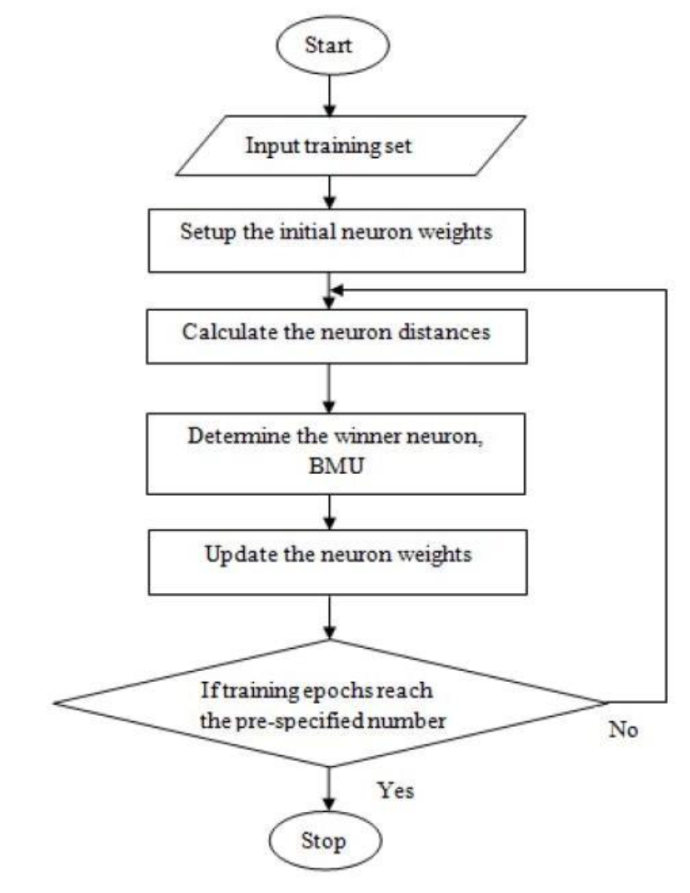
\includegraphics[width=0.7\textwidth]{Gambar/gambar5.1.png}
        \caption{Algoritma Pembelajaran SOM}
    \end{figure}

    SOM terdiri dari sekumpulan neuron buatan, masing-masing terkait dengan vektor kamus kode dengan dimensi yang sama dengan input, yang mewakili struktur topologi data berdimensi tinggi \citep{Cabanes2012}. Gambar 1 menampilkan ringkasan algoritma pembelajaran SOM \citep{Fuertes2010}. Gambar ini menunjukkan bahwa setiap instance data masukan akan diproses berdasarkan jumlah epoch pelatihan yang telah ditentukan sebelumnya. Selama pelatihan SOM, jarak antara data masukan dan vektor buku kode dihitung untuk menentukan neuron pemenang, yang disebut unit pencocokan terbaik (BMU).

    Sifat matematis perilaku pembelajaran SOM telah dijelaskan secara rinci dalam \citep{Cabanes2012} tetapi akan diuraikan secara singkat sebagai berikut :

    Misalkan $X(t) = x(x_1, x_2, \ldots, x_n)$ adalah vektor masukan berdimensi $n$, dan
    $w_i(t) = (w_{i1}, w_{i2}, \ldots, w_{im})$ adalah vektor referensi yang terkait dengan neuron ke-$i$ pada waktu $t$.

    \[
        w_{\text{in}} = \min_i \| x(t) - w_i(t) \|
    \]

    Dalam Persamaan (1), $w_{\text{in}}$ adalah indeks Unit Pencocokan Terbaik (BMU).
    
    Setelah menentukan BMU, setiap vektor referensi dimodifikasi sebagai berikut.

    \[
        w_i(t + 1) = w_i(t) + \alpha(t) \, h(w_{\text{in}}, i, t) \, [x(t) - w_i(t)]
    \]

    Dalam Persamaan~(2), $\alpha(t)$ merujuk pada laju pembelajaran yang nilainya menurun seiring dengan waktu iterasi, sedangkan $h(w_{\text{in}}, i, t)$ merujuk pada fungsi tetangga yang merupakan fungsi monoton menurun terhadap jarak geometris antara \textit{Best Matching Unit} (BMU) dan neuron ke-$j$ pada peta. 

    Fungsi tetangga ini memastikan pelestarian struktur topologis dari data masukan berdimensi tinggi ke dalam peta berdimensi rendah.
    
\section{Eksperimen Visualisasi}

    Untuk eksperimen dalam makalah ini, data yang digunakan terdiri dari karakteristik pembelajaran 39 siswa pada 5 tingkat masalah, di mana tingkat 1 terdiri dari 12 soal, tingkat 2 terdiri dari 3 soal, tingkat 3 terdiri dari 12 soal, tingkat 4 terdiri dari 3 soal, dan tingkat 5 terdiri dari 12 soal. Level 2 dan 4 tidak digunakan karena hanya terdiri dari 3 soal \citep{Hirashima2007}.

    \textit{MONSAKUN} sendiri dirancang sebagai media pembelajaran interaktif untuk pemecahan masalah \citep{Hirashima2014}. \textit{MONSAKUN} mencatat aktivitas siswa selama kegiatan pemecahan masalah mereka, yang mencakup fitur-fitur berikut:

    \begin{enumerate}
        \item Nomor Induk Mahasiswa: Ini berisi variabel kunci utama yang membedakan setiap mahasiswa.
        \item Durasi: Mengandung waktu yang dibutuhkan siswa untuk menyelesaikan tugas dalam detik.
        \item Langkah: Mengandung jumlah langkah (set dan remove) yang dilakukan oleh siswa.
        \item Set: Ini berisi jumlah langkah set yang dilakukan oleh siswa.
        \item Menghapus: Mengandung jumlah langkah menghapus yang dilakukan oleh siswa.
        \item C1: Mengandung jumlah penggunaan kartu 1 oleh siswa.
        \item C2: Menampilkan jumlah penggunaan kartu 2 oleh siswa.
        \item C3: Mengandung jumlah penggunaan kartu 3 oleh siswa
        \item C4: Menampilkan jumlah penggunaan kartu 4 oleh siswa
        \item C5: Mengandung jumlah penggunaan kartu 5 oleh siswa
        \item C6: Mengandung jumlah penggunaan kartu 6 oleh siswa
        \item Unique: Mengandung jumlah kombinasi kartu unik yang digunakan oleh siswa
        \item Error: Mengandung jumlah kesalahan selama pelaksanaan tugas
    \end{enumerate}

    Kami melatih SOM untuk setiap level pada setiap tugas untuk memvisualisasikan karakteristik siswa. Gambar 2 memvisualisasikan distribusi karakteristik siswa untuk tugas 1 (level 1). Setiap angka pada peta mewakili ID siswa tertentu. Misalnya, kita dapat secara intuitif memahami bahwa siswa 2 memiliki kesamaan perilaku belajar dengan siswa 16 tetapi sangat berbeda dari siswa 22. Di sudut kiri bawah peta, kita dapat mengamati sekelompok siswa dengan kesamaan perilaku belajar yang serupa, sementara di sisi kanan peta, kita dapat mengamati tiga siswa (31, 14, 22) yang secara jelas berbeda dari siswa lain. Siswa 7 (lingkaran biru) adalah siswa dengan kinerja terburuk. Dapat diamati bahwa siswa tersebut memiliki kesamaan dengan banyak siswa lain (6, 20, 33) dan berpotensi dapat memperoleh manfaat dengan meniru perilaku belajar mereka.

    \begin{figure}[H]
        \centering
        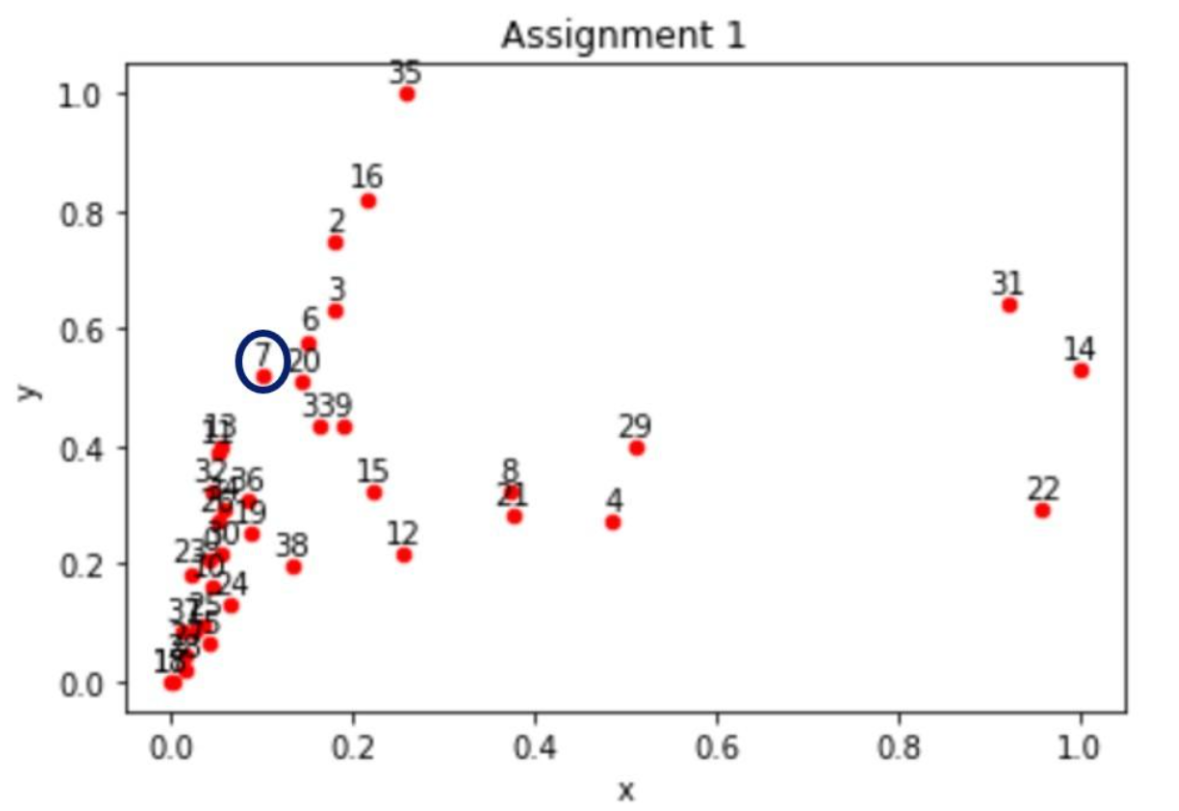
\includegraphics[width=0.7\textwidth]{Gambar/gambar5.2.png}
        \caption{Visualisasi SOM Siswa pada Tugas 1 Level 1}
    \end{figure}

    Gambar 3 menampilkan distribusi karakteristik siswa untuk tugas 4 (tingkat 1). Setiap angka pada peta mewakili ID siswa tertentu. Di sini, misalnya, kita dapat secara intuitif memahami bahwa siswa 32 memiliki kesamaan perilaku belajar dengan siswa 7 tetapi sangat berbeda dari siswa 28. Di sudut kiri bawah peta, kita dapat mengamati sekelompok siswa dengan kesamaan perilaku belajar yang serupa, sementara di sisi kanan peta, kita dapat mengamati satu siswa (28) yang secara jelas berbeda dari siswa lainnya. Siswa 13 (lingkaran biru) adalah siswa dengan kinerja terburuk

    Dapat diamati bahwa siswa tersebut memiliki kesamaan dengan banyak siswa lain (24, 10, 30) dan berpotensi mendapatkan manfaat dengan meniru perilaku belajar mereka.

    \begin{figure}[H]
        \centering
        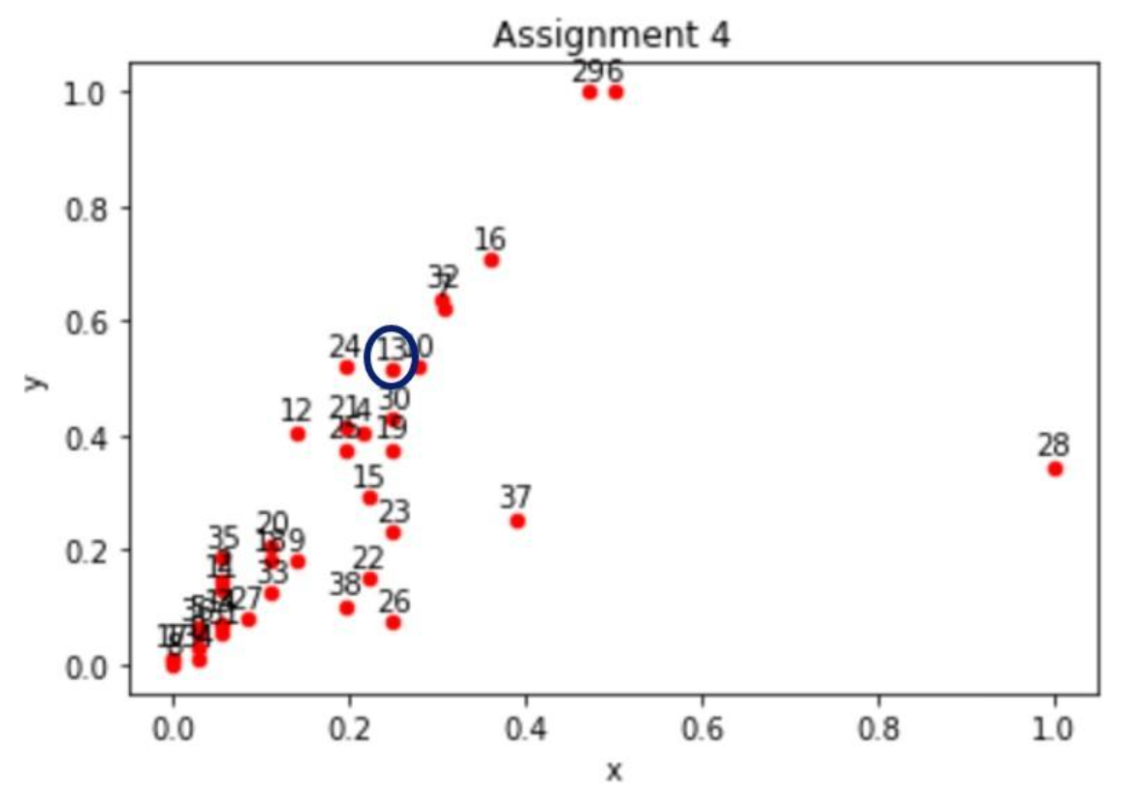
\includegraphics[width=0.7\textwidth]{Gambar/gambar5.3.png}
        \caption{Visualisasi SOM Siswa pada Tugas 4 Level 1}
    \end{figure}

\section{Kesimpulan}

    Dalam makalah ini, kami telah melakukan eksperimen awal dalam memvisualisasikan karakteristik siswa. Meskipun peta yang dihasilkan intuitif dan dalam beberapa hal informatif untuk memahami karakteristik siswa, peta tersebut hanya memberikan gambaran sekilas untuk satu tes tertentu. Dalam penelitian kami selanjutnya, kami berencana mengintegrasikan informasi dari peta ini ke dalam grafik kesamaan yang lebih baik menggambarkan kesamaan siswa secara hierarkis. Kami kemudian akan menggunakan grafik-grafik ini untuk secara otomatis menghasilkan saran pembelajaran yang dapat disesuaikan secara manual oleh guru dengan tujuan utama membantu siswa.
    
    Kami juga berencana untuk membangun antarmuka yang intuitif dan interaktif yang memungkinkan guru untuk dengan mudah menggunakan alat saran ini. Sistem penasihat akan diimplementasikan dan dievaluasi secara menyeluruh di Indonesia

\chapter{SISTEM BIMBINGAN BELAJAR BERBASIS KESAMAAN SISWA}

\section{Pendahuluan}

    Banyak negara berkembang menghadapi ketidakseimbangan dalam rasio siswa- guru. Misalnya, pada tahun 2018, di antara negara-negara ASEAN, rasio untuk Filipina adalah 36, Thailand 24, dan Indonesia 15. Di antara enam anggota, Brunei Darussalam memiliki jumlah siswa per guru terendah, yaitu 8 , Malaysia 11, dan Singapura 11,6. Rasio siswa-guru y a n g lebih seimbang sangat penting untuk memastikan kualitas pendidikan. Ketidakseimbangan rasio guru-siswa dapat memiliki beberapa dampak signifikan: penurunan kualitas pengajaran, penurunan prestasi akademik, kesulitan dalam pengelolaan kelas, stres dan kelelahan guru, kurangnya kesempatan partisipasi, dan ketimpangan pendidikan \citep{Ancho2021}. Hal ini membebani guru di negara-negara dengan rasio siswa-guru yang tinggi, seperti Indonesia, sehingga guru tidak selalu dapat memberikan perhatian yang cukup kepada siswa dan melaksanakan proses pendidikan yang detail untuk setiap siswa.

    Dalam beberapa tahun terakhir, proliferasi platform pembelajaran daring telah secara signifikan memudahkan akses terhadap data pendidikan. Platform pembelajaran daring telah menghasilkan big data. Data ini dapat diproses dan disajikan, serta informasi yang dapat digunakan untuk menentukan strategi pembelajaran dan saran bagi siswa melalui alat bantu pembelajaran. Alat bantu pembelajaran yang menyediakan strategi pembelajaran untuk setiap siswa sangat penting untuk mendukung proses pendidikan, terutama dengan rasio siswa-guru yang buruk. Alat bantu pembelajaran ini penting untuk didesain agar memudahkan guru dalam memberikan bimbingan yang relevan dengan kebutuhan siswa, dengan fokus khusus pada siswa yang kurang berprestasi.
    
    Beberapa sistem bimbingan akademik telah diterapkan di berbagai lembaga pendidikan, sebagai berikut: sistem rekomendasi mata kuliah dan bimbingan akademik sangat penting bagi lembaga pendidikan tinggi untuk mengelola penjadwalan, pendaftaran, dan bimbingan di tengah meningkatnya jumlah mahasiswa dan beragamnya pilihan kurikulum. Sistem ini memungkinkan mahasiswa mendaftar mata kuliah tanpa khawatir tentang ketersediaan, memfasilitasi keselarasan dengan teman sekelas yang berada di jalur akademik dan tingkat kualifikasi yang sama \citep{Daramola2014}. Mekanisme bimbingan lanjutan untuk membantu mahasiswa sarjana selama pendaftaran berdasarkan penambangan data dan penambangan aturan asosiasi untuk menganalisis ketergantungan antar mata kuliah dan memberikan panduan dalam memilih mata kuliah yang secara historis menghasilkan kinerja mahasiswa yang memuaskan. Meskipun belum sepenuhnya otomatis, sistem ini dapat secara signifikan mengurangi waktu yang dihabiskan oleh penasihat untuk membantu banyak mahasiswa. Selain itu, mahasiswa dapat membuat pilihan mata kuliah yang tepat berdasarkan hubungan antar mata kuliah, meniru proses pengambilan keputusan di dunia nyata \citep{keylist}.
    
    Studi ini mengembangkan kerangka kerja Penasihat Mahasiswa Otomatis menggunakan algoritma C4.5 untuk memprediksi pilihan jurusan mahasiswa tahun pertama, dengan tujuan meningkatkan kinerja akademik. Mereka mengelompokkan mahasiswa menggunakan algoritma k-means dan menghitung tingkat keberhasilan untuk setiap departemen dalam kelompok-kelompok tersebut. Tingkat keberhasilan ini mengarahkan mahasiswa ke jurusan dengan probabilitas keberhasilan tertinggi \citep{MohamedAly2013}. Keberadaan daring secara bertahap menjadi hal yang wajib bagi semua lembaga pendidikan. Oleh karena itu, sejumlah besar karya ilmiah kini dapat diakses secara daring. Meskipun demikian, penasihat akademik masih kesulitan untuk mengawasi dan membimbing kemajuan akademik serta aktivitas mahasiswa mereka dengan sukses, meskipun tren ini terus berkembang.

    Penggunaan teknologi informasi untuk tujuan pendidikan. Tujuan sistem ini bukanlah untuk menggantikan peran penasihat manusia (staf). Sebaliknya, sistem ini membebaskan mahasiswa untuk fokus pada hal-hal penting terkait pendaftaran mata kuliah dan memberikan akses terbuka kepada penasihat profesional, sehingga mengurangi beban kerja penasihat manusia. Dengan menggunakan teknologi berbasis web, makalah ini menawarkan sistem penasihat yang ditingkatkan untuk tujuan pendidikan \citep{NsikanAbasi2016}.
    
    Peneliti ini memperkenalkan konsep "grafik perangkap" untuk mengukur tingkat keterlibatan dan pemahaman siswa dalam lingkungan pembelajaran pemecahan masalah. Grafik perangkap mengidentifikasi kesalahan umum atau "perangkap" yang dihadapi siswa. Nilai perangkap yang dihasilkan dari grafik ini menjadi dasar untuk mendeteksi kondisi perangkap, yang menandakan situasi di mana siswa mungkin kesulitan memahami struktur masalah. Namun, penelitian ini masih berada pada tahap awal dan memerlukan analisis lebih lanjut, termasuk meninjau visualisasi untuk setiap tugas. Studi yang diusulkan bertujuan untuk mengembangkan sistem penasihat pembelajaran yang lebih intuitif yang dapat digunakan guru dengan mudah tanpa harus mahir dalam pengolahan data. Studi sebelumnya yang berbeda menggunakan MONSAKUN, yaitu platform pembelajaran daring untuk anak sekolah dasar yang belajar aritmatika di Jepang \citep{Hirashima2014}. Di platform ini, siswa diberikan kumpulan soal yang sama dan dapat mengembangkan strategi sendiri untuk memecahkan soal. Aktivitas belajar siswa di MONSAKUN direkam sebagai data logbook. Data ini juga dapat digunakan untuk berbagai tujuan, termasuk identifikasi perilaku belajar siswa, peningkatan kinerja melalui pemecahan masalah, dan perbaikan lingkungan belajar secara keseluruhan \citep{Supianto2016}.
    
    Banyak komunitas penelitian telah menunjukkan minat yang signifikan dalam memprediksi perilaku siswa dan mengekstrak wawasan berharga dari pola-pola tersebut, didukung oleh ketersediaan data pendidikan yang luas. Penggunaan informasi sering kali dipandu oleh komunitas analitik pembelajaran, yang menekankan pada peningkatan lingkungan pembelajaran secara keseluruhan, daripada hanya berfokus pada peningkatan prestasi siswa \citep{Schumacher2018}. Kolaborasi interdisipliner dalam penerapan dan analisis data pembelajaran telah menghasilkan berbagai terminologi, termasuk analisis pembelajaran, analisis akademik, dan analisis prediktif \citep{Viberg2018}. Perbedaan strategi yang digunakan siswa dalam memecahkan masalah berasal dari cara dan proses berpikir yang berbeda-beda. Setelah itu, metode yang mereka gunakan untuk memecahkan masalah tersebut didokumentasikan sebagai data karakteristik pembelajaran, di mana setiap siswa ditampilkan sebagai titik dalam ruang berdimensi tinggi dengan dimensi yang menunjukkan jumlah fitur pembelajaran \citep{Kreuseler2002}.

    \begin{figure}[H]
        \centering
        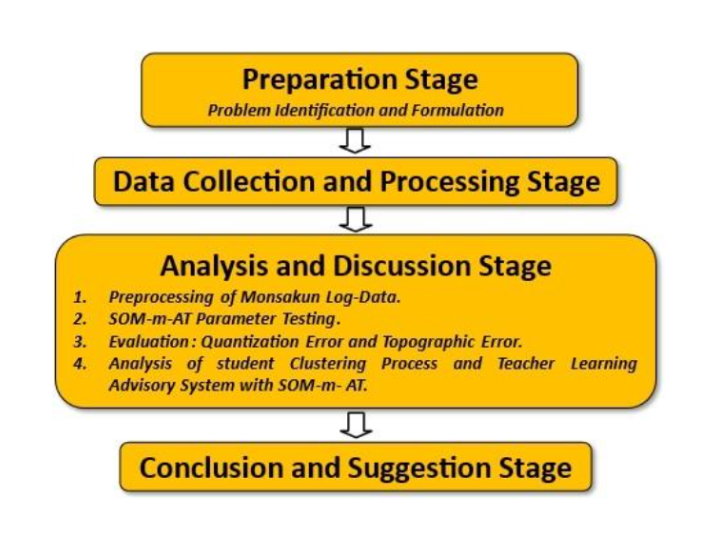
\includegraphics[width=0.7\textwidth]{Gambar/gambar6.1.png}
        \caption{Metodologi Penelitian}
    \end{figure}

    Karena MONSAKUN menyediakan data berdimensi tinggi, Peta Organisasi Diri (SOM) digunakan untuk mereduksinya menjadi dua dimensi \citep{Kohonen2002} guna visualisasi intuitif dan penemuan kemiripan. Peta dua dimensi yang dihasilkan oleh SOM digunakan untuk menginterpretasikan dan mengidentifikasi kesamaan antar siswa. Algoritma yang digunakan dalam sistem penasihat pembelajaran siswa ini berfokus pada pengenalan algoritma baru, Self-Organizing Maps-m-Ary Tree (SOM-m-AT).

    Penelitian sebelumnya terkait kombinasi SOM dan teori graf telah diusulkan dalam pendekatan partisi graf untuk pengelompokan SOM \citep{Silva2011}. Dalam studi ini, pohon m-Ary dalam SOM digunakan untuk menganalisis hasil pengelompokan siswa dan memberikan umpan balik kepada guru.
    
    Penelitian ini berusaha mengembangkan alat pendidikan yang memungkinkan guru menganalisis perilaku belajar siswa secara intuitif dan selanjutnya membantu guru menghasilkan saran yang bermakna, terutama untuk siswa dengan kinerja rendah. Hal ini dimungkinkan oleh ketersediaan data belajar siswa yang diperoleh melalui platform belajar digital. Tujuan penelitian ini adalah sebagai berikut:
    
    Pertama, studi ini mengelompokkan siswa dengan karakteristik belajar yang serupa dari suatu kluster, sementara siswa yang berbeda berasal dari kluster yang berbeda dan dikelompokkan dalam kluster lain. Karena tujuan kami adalah mengembangkan alat analitis yang intuitif, kami perlu menyajikan kluster-kluster ini secara intuitif sehingga guru yang tidak necessarily ahli dalam analisis data dapat memahaminya. Oleh karena itu, kami mengadopsi teknik visualisasi melalui pengurangan dimensi.
    
    Kedua, kami membangun Sistem Penasihat Pembelajaran (LAS) yang diusulkan berdasarkan kesamaan siswa menggunakan SOM-m-AT. Analisis matematis dilakukan pada data eksperimental dari MONSAKUN, platform pembelajaran yang digunakan di Jepang untuk mengajarkan aritmatika kepada siswa sekolah dasar. Hasilnya menunjukkan seberapa efektif strategi yang diusulkan.
    
    Metodologi penelitian digambarkan dalam Gambar 1. Metodologi penelitian ini dibagi menjadi empat tahap: Tahap persiapan; pengumpulan data dan pengolahan data; tahap analisis dan pembahasan, yang meliputi :

    \begin{enumerate}
        \item Prasunting Data Log MONSAKUN,
        \item Pengujian parameter SOM-m-AT,
        \item Evaluasi: Kesalahan kuantisasi dan kesalahan topografi,
        \item Analisis proses pengelompokan siswa dan Sistem Penasihat Pembelajaran Guru dengan SOM-m-AT,
    \end{enumerate}

    Sedangkan tahap terakhir adalah kesimpulan dan saran. Berikut adalah noveltas utama dalam makalah ini: Untuk menciptakan sistem penasihat pembelajaran, teknik SOM-m-AT yang menggabungkan manfaat SOM dan grafik m-AT ditawarkan. Data dari MONSAKUN, kerangka kerja pembelajaran digital Jepang yang menekankan pemecahan masalah dalam pembelajaran matematika sekolah dasar, digunakan dalam studi ini.
    
    Bagian-bagian selanjutnya dari makalah ini disusun sebagai berikut: Bagian 2 memberikan gambaran singkat tentang peta self-organizing dan struktur pohon yang digunakan dalam penelitian ini. Bagian 3 menjelaskan eksperimen teknis yang dilakukan. Bagian 4 menyajikan dan menganalisis hasil eksperimen, sementara Bagian 5 menyimpulkan makalah dan mengusulkan arah penelitian di masa depan.

\section{Peta SOM dan Struktur Pohon m-AT}

    Kohonen menciptakan SOM, jenis jaringan saraf tiruan (JST), pada tahun 1980-an. SOM telah diterapkan secara efektif di beberapa bidang, termasuk kuantisasi vektor, pengenalan pola, analisis teks lengkap, analisis gambar, regresi, dan diagnostik kesalahan \citep{Kohonen1998b}. SOM, sebagai jaringan saraf, memetakan data berdimensi tinggi ke ruang berdimensi lebih rendah, yang diwakili oleh kisi neuron yang terhubung ke vektor kamus dengan dimensi yang sama dengan data input. Proses pembelajaran SOM dijelaskan dalam Gambar 2.

    Sifat matematis perilaku pembelajaran SOM telah dijelaskan secara rinci \citep{Cabanes2012}, \citep{Fuertes2010} tetapi akan diuraikan secara singkat sebagai berikut :

    Misalkan $X(t) = (x_1, x_2, \ldots, x_n)$ adalah vektor input berdimensi $n$, dan 
    $W_i(t) = (w_{i1}, w_{i2}, \ldots, w_{in})$ adalah vektor kamus kode yang terkait dengan neuron ke-$i$ pada waktu $t$, 
    sedangkan indeks \textit{Best Matching Unit} (BMU) adalah $w_{\text{in}}$, seperti yang ditentukan dalam Persamaan~(2.1).

    \[
        w_{\text{in}} = \arg \min_i \| X(t) - W_i(t) \|
    \]

    \begin{figure}[H]
        \centering
        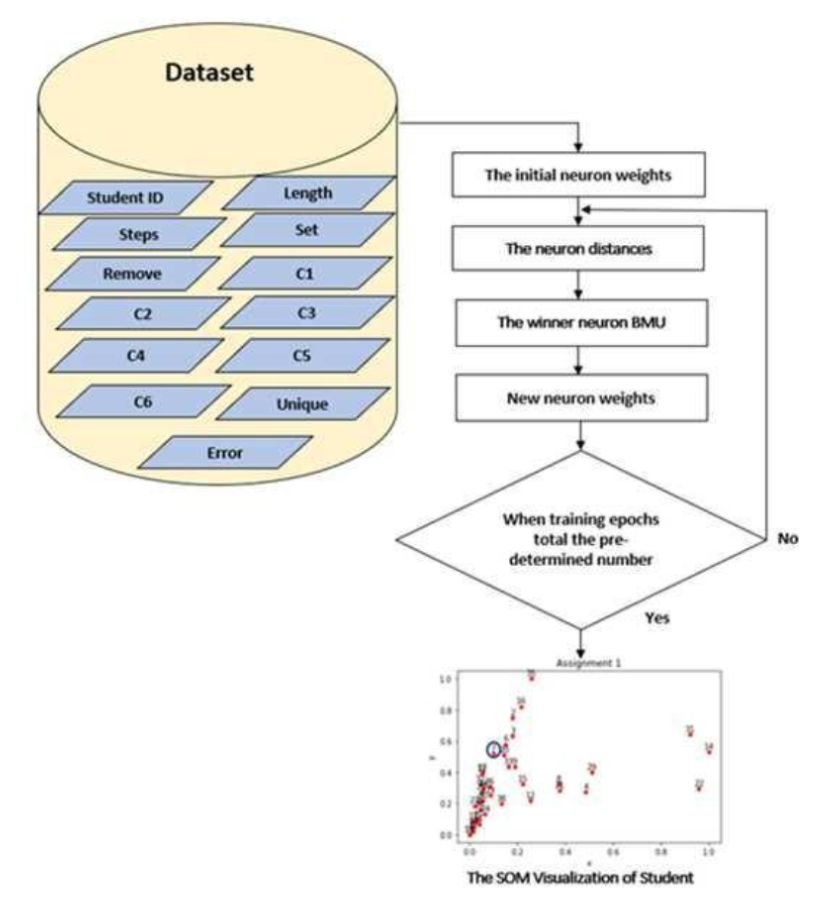
\includegraphics[width=0.7\textwidth]{Gambar/gambar6.2.png}
        \caption{Algoritma Pembelajaran SOM}
    \end{figure}

    Setelah menentukan BMU, setiap vektor referensi dimodifikasi sebagai berikut.

    \[
        W_j(t + 1) = W_j(t) + \alpha(t) \, h(w_{\text{in}}, j, t) \, [X(t) - W_j(t)]
    \]

    Dalam Persamaan (2.2), $\alpha(t)$ menunjukkan laju pembelajaran yang menurun, sedangkan 
    $h(w_{\text{in}}, j, t)$ merupakan fungsi tetangga yang menurun seiring dengan bertambahnya jarak 
    geometris antara neuron pemenang (\textit{Best Matching Unit} atau BMU) dan neuron ke-$j$ pada peta. 
    Fungsi tetangga menjamin bahwa masukan berdimensi tinggi yang dipetakan ke ruang berdimensi rendah 
    tetap mempertahankan struktur topologisnya. 

    Fungsi ini umumnya merupakan fungsi Gaussian yang dapat didefinisikan sebagai:
    \[
        h_{cj}(t) = \exp\!\left(-\frac{\|r_c - r_j\|^2}{2\sigma^2(t)}\right)
    \]

    Di sini, $\text{coord}(w_{\text{in}})$ dan $\text{coord}(j)$ mewakili koordinat \textit{Best Matching Unit} (BMU) dan neuron ke-$j$, sedangkan $\sigma(t)$ adalah parameter skala yang ditentukan secara empiris.

    Ada banyak algoritma untuk metode pengurangan dimensi (DR), di mana salah satu algoritma DR tertua adalah Analisis Komponen Utama (PCA). PCA adalah algoritma yang mengurangi dimensi data dengan mengidentifikasi yang disebut Komponen Utama \citep{Steffens1983}. Meskipun PCA dapat diimplementasikan dengan mudah, algoritma ini dibatasi oleh linearitas dalam menentukan Komponen Utama. Oleh karena itu, PCA mungkin tidak dapat menggambarkan non-linearitas dalam data secara memadai. Algoritma pengurangan dimensi konvensional lainnya adalah Analisis Diskriminan Linier (LDA). Mirip dengan PCA, LDA juga merupakan metode DR yang dibatasi oleh linearitas, tetapi mempertimbangkan label kelas data \citep{Hartono2017}. Dalam studi ini, kami menggunakan Peta Organisasi Diri (SOM) karena kemudahan implementasinya tanpa dibatasi oleh linearitas. Selama beberapa dekade terakhir, berbagai varian SOM telah digunakan secara luas untuk analisis dan visualisasi data, misalnya: \citep{Ahmad2018}, \citep{Bara2018}, \citep{Ahmad2018}. Dalam studi ini, SOM menghasilkan peta 2D yang mempertahankan hubungan topologis dalam data pembelajaran berdimensi tinggi. Siswa dengan karakteristik pembelajaran serupa dikelompokkan, sementara yang memiliki karakteristik berbeda ditempatkan lebih jauh. Tujuan utama studi ini adalah mengidentifikasi siswa yang mengalami kesulitan akademis, karena mereka dapat memperoleh manfaat terbesar dari dukungan guru yang ditargetkan. Dengan memvisualisasikan siswa-siswa ini dan teman sebayanya yang menunjukkan strategi belajar efektif di dekat mereka pada peta, pendidik dapat memfasilitasi pembelajaran antar teman sebaya. Tujuannya adalah mendorong siswa yang mengalami kesulitan untuk mengadopsi kebiasaan belajar efektif dari teman sebayanya yang lebih sukses. Mengingat kesamaan gaya belajar, siswa-siswa ini dapat melakukan penyesuaian bertahap pada pendekatan mereka tanpa membutuhkan perubahan yang signifikan. Diperkirakan bahwa penerapan konsisten strategi ini pada berbagai tugas akan membawa perbaikan bertahap pada siswa.

    Temuan studi menunjukkan bahwa SOM menghasilkan hasil yang memadai dan mampu memenuhi hasil yang diinginkan. Apakah strategi ini juga efektif dalam membagi siswa ke dalam kelompok berdasarkan materi pembelajaran digital yang telah mereka gunakan? Hal ini menimbulkan pertanyaan apakah pertanyaan penelitian, yang akan menggunakan teknik penilaian kesalahan kuantisasi (QE) dan kesalahan topografi (TE) \citep{Breard2018}, berkaitan dengan kinerja SOM dalam hal data pendidikan. Fokus utama studi ini adalah bagaimana menggunakan algoritma SOM untuk mengevaluasi perilaku siswa saat menyelesaikan tugas pada media pembelajaran. Untuk memahami tantangan belajar siswa dengan lebih baik dan memberikan umpan balik pembelajaran yang lebih tepat dan tepat waktu, diharapkan jawaban atas pertanyaan penelitian ini akan tinggi. Setelah pembangkitan peta dimensi rendah siswa, kesamaan mereka perlu diidentifikasi. Meskipun SOM menawarkan visualisasi intuitif kesamaan, ia tidak secara eksplisit menyediakan ukuran kesamaan. Dalam hal ini, kami menggunakan m-Ary Tree (m- AT) sebagai ukuran eksplisit kesamaan siswa, di mana seorang siswa diwakili oleh sebuah node. Siswa lain yang berada di dekat node tersebut pada peta dianggap sebagai anak dari node tersebut. Perlu dicatat bahwa SOM membentuk peta topologis di mana jarak mewakili ketidaksamaan. Oleh karena itu, ukuran kesamaan yang diperlukan untuk membuat m-AT dapat dihitung langsung dari SOM. Ukuran kesamaan ini lebih intuitif daripada pengukuran langsung data asli. m-Ary Trees (m-AT) memungkinkan setiap node memiliki maksimal m-anak yang mewakili pola belajar siswa \citep{Supianto2021}.
    
    Setelah pembangkitan peta dimensi rendah dari seorang siswa, kesamaan di antara mereka perlu diidentifikasi. Meskipun SOM menawarkan visualisasi intuitif dari kesamaan, ia tidak secara eksplisit menyediakan ukuran kesamaan. Dalam hal ini, kami menggunakan m-Ary Tree (m-AT) sebagai ukuran eksplisit kesamaan siswa, di mana seorang siswa tertentu diwakili oleh sebuah node. Siswa lain yang berada di dekat siswa tersebut pada peta dianggap sebagai anak dari node tersebut. Di sini, perlu dicatat bahwa SOM membentuk peta topologis di mana jarak mewakili ketidaksamaan. Oleh karena itu, ukuran kesamaan yang diperlukan untuk membuat m-AT dapat dihitung langsung dari SOM. Ukuran kesamaan ini lebih intuitif daripada pengukuran langsung data asli. m-Ary Trees (m-AT) memungkinkan setiap node memiliki maksimal m-anak.

    Diharapkan pendekatan yang diusulkan dapat mengelompokkan dan memvisualisasikan karakteristik belajar siswa sekolah dasar di berbagai proyek matematika online. Penelitian ini menggunakan log data MONSAKUN, sebuah platform pembelajaran digital yang berfokus pada latihan aritmatika melalui penyajian masalah berbasis narasi, sebagai studi kasus.

    Penerapan m-AT dalam studi kami berfungsi sebagai kerangka kerja dasar untuk mengorganisir dan menganalisis karakteristik belajar siswa sekolah dasar yang terlibat dalam latihan matematika di lingkungan belajar digital MONSAKUN. Dengan memanfaatkan struktur hierarkis m-Ary Trees, kami dapat mengkategorikan dan mengelompokkan data kinerja siswa secara efisien, memungkinkan analisis mendalam terhadap karakteristik belajar. Kemampuan penyesuaian faktor cabang 'm' memungkinkan kami menyesuaikan analisis dengan pencapaian belajar siswa dan memetakan hasilnya secara sesuai. Dengan mengintegrasikan m-AT dengan pendekatan pemecahan masalah dan integrasi kalimat matematika, kami bertujuan untuk mengungkap wawasan yang dapat ditindaklanjuti untuk membantu guru dengan memberikan saran.

\section{Hasil dan Pembahasan}

    Pada bagian ini, kami menjelaskan landasan teoritis pengembangan ini. Karakteristik pembelajaran dari 39 siswa pada lima tingkat kesulitan—tingkat 1 dengan 12 soal, tingkat 2 dengan tiga soal, tingkat 3 dengan 12 soal, tingkat 3 dengan tiga soal, tingkat 4 dengan tiga soal, dan tingkat 5 dengan 12 soal— digunakan sebagai data untuk eksperimen dalam artikel ini. Karena level 2 dan 4 hanya memiliki tiga soal, keduanya tidak digunakan \citep{Hirashima2014} MONSAKUN mencatat aktivitas siswa selama kegiatan pemecahan masalah, yang mencakup fitur-fitur berikut:

    \begin{enumerate}
        \item ID Siswa. Ini mencakup variabel kunci utama yang membedakan setiap siswa.
        \item Durasi. Mencatat waktu yang dibutuhkan untuk menyelesaikan tugas dalam detik.
        \item Langkah. Ini terdiri dari jumlah langkah (set dan remove) yang dilakukan.
        \item Set. Ini mencakup jumlah langkah set yang dilakukan oleh siswa.
        \item Hapus. Angka ini menunjukkan jumlah langkah penghapusan yang dilakukan oleh siswa.
        \item C1, C2, C3, C4, C5, C6. Mereka mencakup jumlah kartu soal cerita aritmatika yang digunakan dengan indeks =1-6.
        \item Unik. Ini mencakup jumlah susunan kartu unik yang digunakan oleh siswa.
        \item Kesalahan. Menunjukkan jumlah kesalahan yang terjadi selama pengerjaan tugas.
    \end{enumerate}

    Dari hasil eksperimen SOM dalam studi ini, QE dan TE masing-masing sebesar 0.1556 dan 0.1666 pada 3. Hasil ini menunjukkan bahwa SOM menangkap struktur kesamaan sampel dalam representasi dimensi rendah mereka.
        
    Kami melatih SOM untuk setiap level pada setiap tugas untuk memvisualisasikan karakteristik siswa. Gambar 3 memvisualisasikan distribusi karakteristik siswa untuk tugas 1 (level 1). Setiap angka pada peta mewakili ID siswa tertentu. Di sini, misalnya, kita dapat secara intuitif memahami bahwa siswa 2 memiliki kesamaan perilaku belajar dengan siswa 16 tetapi sangat berbeda dari siswa 22. Di sudut kiri bawah peta, kita dapat mengamati sekelompok siswa dengan kesamaan perilaku belajar yang serupa, sementara di sisi kanan peta, kita dapat mengamati tiga siswa (31, 14, 22) yang secara jelas berbeda dari siswa lainnya. Dari hasil di atas, SOM dapat memberikan informasi intuitif secara visual (hanya dengan melihat grafik), hal ini sangat penting bagi guru yang tidak familiar dengan ilmu data untuk mengetahui Pola Belajar Siswa. Dari sini, penelitian SOM memiliki makna.
    
    Siswa 7 (lingkaran biru) adalah siswa dengan performa terburuk. Untuk tugas 1 (level 1), siswa ini memiliki kesamaan dengan banyak siswa lain (6, 20, 33) dan berpotensi mendapatkan manfaat dengan meniru perilaku belajar mereka.
    
    Tujuh kategori kesalahan dalam penyusunan soal yang diidentifikasi oleh model tugas MON-SAKUN adalah: (1) Jenis cerita yang berbeda; (2) Rumus perhitungan yang berbeda; (3) Cerita dan perhitungan yang berbeda; (4) Kesalahan objek; (5) Kesalahan nilai/angka; (6) Kesalahan nilai objek; dan (7) Cerita tidak terbentuk. Gambar 3 menggambarkan diagram alir evaluasi kesalahan. Sistem memberikan pesan umpan balik berdasarkan jenis kesalahan yang dibuat siswa saat menyelesaikan soal yang salah. Gambar ?? menunjukkan diagram alir evaluasi kesalahan MONSAKUN \citep{Supianto2017}.
    
    Contoh urutan keadaan yang telah diselesaikan oleh siswa yang berbeda ditampilkan dalam Gambar 4. Gambar 5(a) menunjukkan bahwa keadaan 010 harus muncul empat kali pada langkah pertama, langkah ke-13, langkah ke-15, dan langkah ke-17 untuk mendapatkan jawaban yang benar. Hal ini sesuai dengan jarak 21, 9, 7, dan 5 pada masing-masing kasus. Kami dapat menemukan nilai jarak untuk keadaan 010 dalam urutan ini dengan mengambil rata-rata dari semua nilai jarak. Nilai jarak keadaan 010 dalam urutan ini adalah 11.

    \begin{figure}[H]
        \centering
        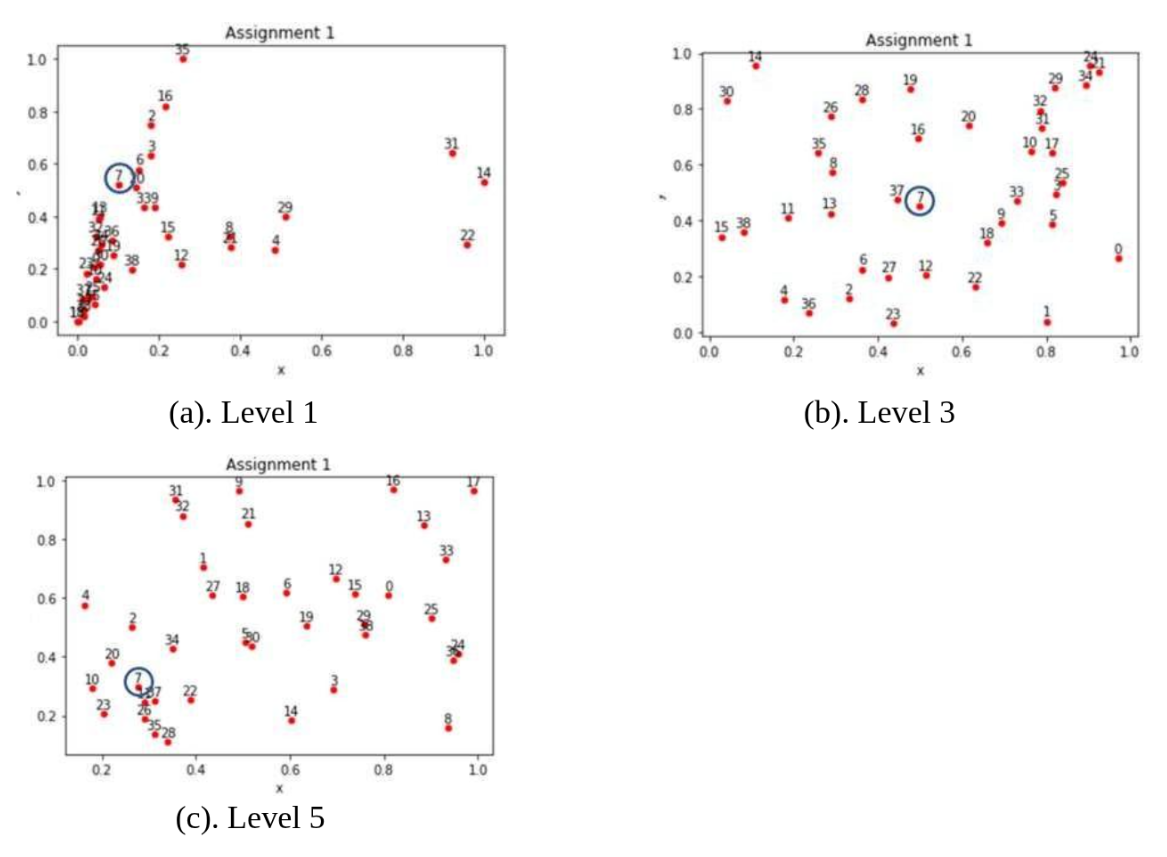
\includegraphics[width=0.7\textwidth]{Gambar/gambar6.3.png}
        \caption{Visualisasi SOM Siswa dalam Tugas 1: Level 1 (a), Level 3 (b), dan Level 5 (c)}
    \end{figure}

    \begin{figure}[H]
        \centering
        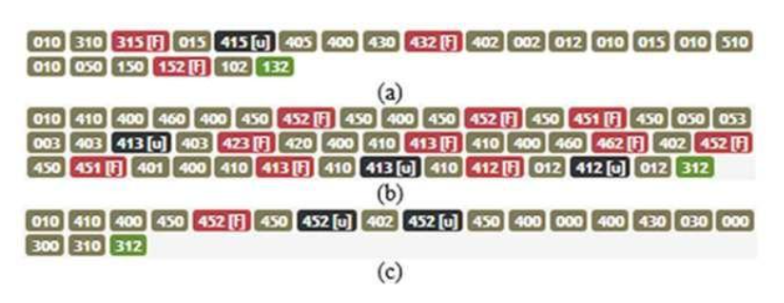
\includegraphics[width=0.7\textwidth]{Gambar/gambar6.4.png}
        \caption{Contoh urutan keadaan (a) Urutan siswa 1 (b) Urutan siswa 2 (c) Urutan siswa 3}
    \end{figure}

    \begin{figure}[H]
        \centering
        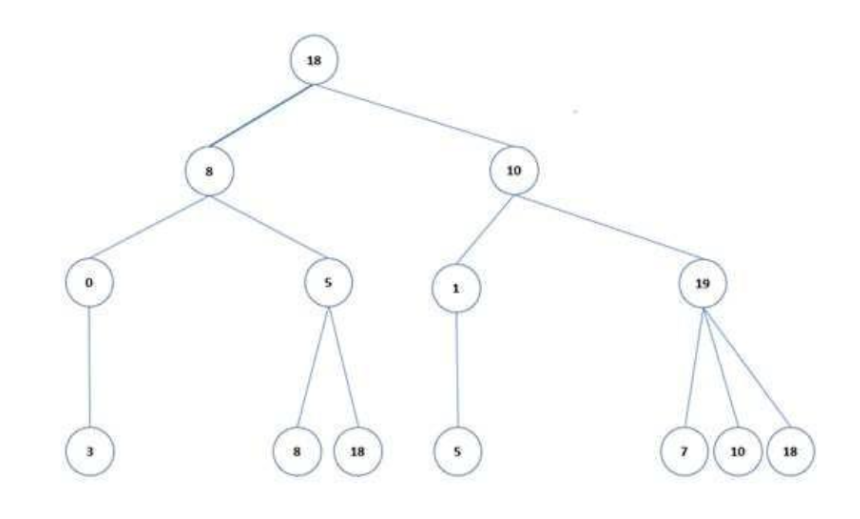
\includegraphics[width=0.7\textwidth]{Gambar/gambar6.5.png}
        \caption{Visualisasi Grafik SOM-m-AT untuk Siswa ke-18}
    \end{figure}

    Eksperimen ini menggunakan algoritma SOM-m-AT yang diusulkan. Gambar 6 menunjukkan struktur pohon yang berpusat pada siswa ke-18. Baris pertama adalah siswa (18), baris kedua menunjukkan bahwa siswa (8,10) memiliki kesamaan belajar tertinggi dengan siswa (18), baris ketiga menunjukkan siswa (0,5) yang memiliki kesamaan dengan siswa (8), dan seterusnya.

    6 menunjukkan struktur pohon yang berpusat pada siswa (7). Baris pertama adalah siswa (7), baris kedua menunjukkan bahwa siswa (3,10,13,19) memiliki kesamaan paling banyak dalam belajar dengan siswa (7), baris ketiga menunjukkan siswa (7,15) yang memiliki kesamaan dengan siswa (3), dan seterusnya. Penentuan urutan siswa dengan prestasi terburuk:

    \begin{enumerate}
        \item Kesalahan terbanyak (Urutan pertama).
        \item C4, C5, C6,
        \item Jumlah langkah, dan
        \item Durasi.
    \end{enumerate}

    1 menunjukkan kriteria siswa terdekat berdasarkan jumlah kesalahan. Siswa 7 dengan kesalahan terburuk adalah 16.
    
    Kemudian temukan siswa terdekat dan terbaik. Ada empat kriteria :

    \begin{enumerate}
        \item Kriteria "Kesalahan": Temukan jenis kesalahan yang dibuat oleh Siswa 7, lalu lihat bagaimana siswa dengan ID terdekat (misalnya: Siswa 10) dapat menyelesaikan masalah dengan melihat urutan langkah-langkah.
            \begin{table}[H]
            \centering
            \caption{Perbandingan Data Log Siswa \citep{Supianto2017} (3, 7, 10, 13, 19)}
            \label{tab:fitur}
            \begin{tabular}{lccccc}
            \toprule
            \textbf{Fitur} & \textbf{ID 3} & \textbf{ID 7} & \textbf{ID 10} & \textbf{ID 13} & \textbf{ID 19} \\
            \midrule
            Panjang     & 542 & 457 & 562 & 755 & 31 \\
            Langkah     & 145 & 114 & 87  & 47  & 7  \\
            Set         & 75  & 60  & 45  & 25  & 5  \\
            Hapus       & 70  & 54  & 42  & 22  & 2  \\
            C1          & 14  & 10  & 5   & 11  & 1  \\
            C2          & 25  & 22  & 12  & 5   & 1  \\
            C3          & 19  & 17  & 35  & 7   & 1  \\
            C4          & 21  & 21  & 3   & 10  & 2  \\
            C5          & 51  & 18  & 16  & 5   & 0  \\
            C6          & 14  & 26  & 15  & 8   & 2  \\
            Unik        & 25  & 42  & 22  & 22  & 7  \\
            Kesalahan   & 11  & 16  & 14  & 6   & 1  \\
            E1          & 6   & 1   & 7   & 6   & 7  \\
            E2          & 1   & 5   & 7   & 6   & 0  \\
            E3          & 1   & 7   & 6   & 7   & 0  \\
            E4          & 7   & 6   & 6   & 7   & 0  \\
            E5          & 1   & 7   & 6   & 7   & 0  \\
            E6          & 7   & 5   & 6   & 5   & 0  \\
            E7          & 7   & 7   & 6   & 0   & 0  \\
            E8          & 7   & 6   & 7   & 0   & 0  \\
            E9          & 6   & 6   & 7   & 0   & 0  \\
            E10         & 1   & 7   & 5   & 0   & 0  \\
            E11         & 7   & 1   & 1   & 0   & 0  \\
            E12         & 0   & 1   & 6   & 0   & 0  \\
            \bottomrule
            \end{tabular}
            \end{table}
            \begin{figure}[H]
                \centering
                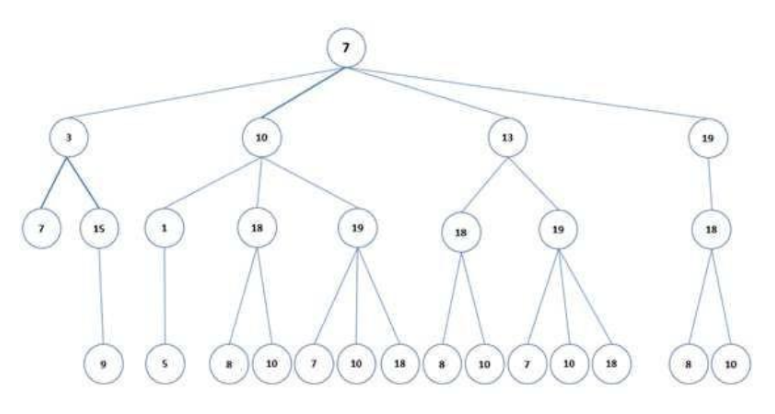
\includegraphics[width=0.7\textwidth]{Gambar/gambar6.6.png}
                \caption{Visualisasi Grafik SOM-m-AT Siswa ke-7}
            \end{figure}
        \item Kriteria “C4”: Kartu 4 adalah kartu dummy yang disediakan secara sengaja untuk menguji pemahaman siswa terhadap ekspresi numerik.
            \begin{itemize}
                \item Tugas: “Berapa jumlah totalnya” yang dapat diselesaikan dengan “8– 3.”
                \item Kalimat untuk setiap kartu, dari yang pertama hingga keenam, adalah:
                    \begin{enumerate}[label=(\alph*)]
                        \item Ada tiga kelinci putih.
                        \item Ada kelinci hitam.
                        \item Ada delapan kelinci putih dan hitam secara keseluruhan.
                        \item Ada delapan kelinci putih.
                        \item Ada tiga kelinci putih lebih banyak daripada kelinci hitam.
                        \item Ada tiga kelinci cokelat.
                    \end{enumerate}
            \end{itemize}
            Dalam situasi ini, banyak siswa merasa bingung, salah mengasosiasikan ekspresi numerik “8” dengan kalimat eksistensi “Ada 8 kelinci putih” daripada kalimat relasional “Ada delapan kelinci putih dan hitam secara keseluruhan.” Siswa masih bingung antara kartu kalimat eksistensi dan relasional, jadi mereka perlu memahami ekspresi numerik.
        \item Kriteria “C5”: Kartu 5 adalah kartu dummy, disediakan secara sengaja untuk menguji pemahaman siswa terhadap cerita. Komposisi ini tidak membentuk jenis cerita tertentu. Siswa menggunakan kartu 5, yang mencerminkan cerita perbandingan, bukan cerita kombinasi. Tugas 1 tentang cerita kombinasi, jadi siswa tidak memahami cerita dalam pertanyaan.
        \item Kriteria “C6”: Kartu 6 adalah kartu dummy, disediakan secara sengaja untuk menguji pemahaman siswa tentang objek. Mahasiswa menggunakan kartu 6, yang menggambarkan objek yang berbeda (kelinci cokelat) daripada kelinci putih atau hitam. Tugas 1 berkaitan dengan kombinasi kelinci putih dan hitam, sehingga mahasiswa tidak memahami kombinasi objek cerita. MONSAKUN ini terdiri dari tiga kartu kalimat yang saling terhubung. Jika ada satu kartu yang tidak terkait, hal itu akan menyebabkan kesalahan.
    \end{enumerate}

    Dari eksperimen, seperti yang ditunjukkan pada Gambar 5 dan 6, kita dapat menemukan bahwa siswa terburuk adalah siswa ke-7 dan ke-18. Kami memilih siswa ke-7 sebagai A sebagai siswa terburuk dibandingkan dengan siswa ke-10 sebagai B , dan siswa ke-3 sebagai C. Kemudian, kami membandingkan fitur-fitur A dan B (atau C). Lihat Tabel I. Dari fitur-fitur yang dihilangkan pada A, B, dan C, kami menemukan fitur-fitur dengan perbedaan nilai terbesar adalah A dan C. Fitur yang dihapus dari C (nilai 70) lebih besar daripada A (nilai 54), sehingga guru dapat menyarankan A untuk meningkatkan nilai fitur yang dihapus ini agar lebih dekat dengan C. Dengan cara yang sama, kita memilih fitur kesalahan di mana C memiliki perbedaan terbesar dari A, sehingga guru harus menyarankan A untuk sedikit meningkatkan skor fitur kesalahan agar lebih dekat dengan skor C. Secara teknis, guru-guru sebaiknya memberikan pelajaran tambahan kepada A tentang soal cerita aritmatika agar kemampuannya lebih mendekati C.

\section{Kesimpulan}

    SOM-m-AT diusulkan sebagai metode baru untuk mempelajari kesamaan siswa dalam sistem bimbingan. Melalui beberapa eksperimen empiris, dapat diamati bahwa metode SOM-m-AT yang diusulkan outperforms SOM dalam efisiensi pembelajaran dan tingkat keberhasilan. Dalam penelitian ini, dengan metode SOM m-AT yang diusulkan, kami menemukan siswa dengan performa terburuk. Kita dapat mengetahui masalah yang dihadapi siswa, sehingga: menemukan siswa terdekat untuk mencoba menyelesaikan masalah yang terkait dengan strategi berpikir. Penelitian ini dapat memberikan informasi kepada guru untuk memberikan umpan balik yang sesuai berdasarkan masalah yang dihadapi siswa.
    
    Dalam penelitian selanjutnya, kami berencana mengintegrasikan informasi yang diperoleh dari peta ini ke dalam grafik kesamaan yang lebih baik menggambarkan kesamaan siswa secara hierarkis. Grafik ini dapat digunakan untuk secara otomatis menghasilkan saran pembelajaran yang dapat disesuaikan secara manual oleh guru dengan tujuan utama membantu siswa. Langkah selanjutnya adalah membangun antarmuka intuitif dan interaktif yang memungkinkan guru menggunakan alat saran ini dengan mudah. Sistem saran ini akan diimplementasikan dan dievaluasi secara menyeluruh di Indonesia.

    Ucapan Terima Kasih. Para penulis ingin mengucapkan terima kasih kepada Profesor Tsukasa Hirashima, Departemen Informatika dan Ilmu Data, Universitas Hiroshima, Jepang, atas dukungannya dalam penelitian ini dengan data MONSAKUN.
\chapter{PERSEPSI GURU SEKOLAH DASAR TERHADAP SISTEM PENASEHAT PEMBELAJARAN BERDASARKAN KEMIRIPAN SISWA}

\section{Pendahuluan}
    Perkembangan teknologi pembelajaran memiliki dampak dan pengaruh yang signifikan terhadap proses pembelajaran siswa. Jepang, yang memiliki salah satu sistem pendidikan terbaik di dunia, mengembangkan berbagai infrastruktur digital pendukung. Jepang sering dijadikan acuan oleh negara-negara berkembang sebagai model untuk meningkatkan kualitas pendidikan \citep{Vicente2024}. Sistem pendidikan Indonesia masih banyak yang dapat dipelajari dari Jepang. Berbeda dengan Jepang, sistem pendidikan di Indonesia belum sepenuhnya menerapkan teknologi pembelajaran di semua sekolah sebagai alat untuk mendukung pembelajaran atau memantau siswa di sekolah.
    
    Salah satu platform teknologi pembelajaran yang dikembangkan di Jepang adalah MONSAKUN dari Universitas Hiroshima untuk anak-anak sekolah dasar \citep{Hirashima2014}. MONSAKUN adalah lingkungan pembelajaran berbasis komputer yang memfasilitasi pembelajaran melalui soal-soal matematika praktis yang melibatkan operasi penjumlahan dan pengurangan tunggal. MONSAKUN bertujuan untuk memberikan penilaian dan umpan balik otomatis atas ujian yang dikirimkan oleh siswa sekolah dasar. Hal ini memungkinkan guru untuk memantau kemajuan individu siswa dan kemajuan kelas secara keseluruhan secara real-time \citep{Hirashima2007}. MONSAKUN menghasilkan data log proses berpikir siswa sekolah dasar dalam belajar aritmatika dasar. Data Log ini kemudian dianalisis dalam \citep{Hasanah2015}.
    
    Dalam studi ini, kami mengembangkan teknik visualisasi menggunakan Self-Organizing Maps (SOM) Kohonen. SOM merupakan alat yang berharga untuk memahami dan menganalisis data berdimensi tinggi \cite{Budayan2009}. Dalam konteks pendidikan, visualisasi merupakan pendekatan intuitif bagi guru yang belum tentu familiar dengan ilmu data. Penelitian sebelumnya yang dilakukan oleh \citep{Tibyani2024,Tibyani2025} membahas tentang mengidentifikasi siswa dengan kinerja rendah dan memberikan bimbingan untuk meningkatkan prestasi akademik mereka melalui analisis data perilaku belajar. Menggunakan metode Self-Organizing Maps-m-Ary Tree (SOM-m-AT), karakteristik belajar siswa dipetakan ke dalam representasi topologis dua dimensi untuk membantu guru mengenali pola belajar mereka. Hasil menunjukkan bahwa siswa dengan perilaku belajar serupa cenderung berkelompok. Representasi dimensi rendah ini kemudian digunakan untuk mengidentifikasi siswa berprestasi rendah dan siswa lain yang memiliki karakteristik belajar serupa tetapi hasil yang lebih baik. Kesamaan belajar kemudian digunakan untuk menghasilkan saran bagi siswa dengan kinerja rendah tanpa harus mengubah pola belajar mereka secara drastis. Karakteristik utama sistem ini terletak pada kemampuannya untuk mengelompokkan siswa berdasarkan kesamaan topologis dalam perilaku belajar, tanpa memerlukan guru untuk memiliki pemahaman mendalam tentang teknik analisis data. Hal ini membuatnya sangat cocok untuk diterapkan di tingkat pendidikan dasar, di mana guru membutuhkan alat intuitif untuk memberikan bimbingan yang terarah.
    
    Untuk mengeksplorasi penerapan nyata pendekatan berbasis data ini dalam konteks pendidikan yang berbeda, penting untuk menganalisis bagaimana sistem semacam ini dipersepsikan oleh pengguna yang dituju—guru. Memahami penerimaan teknologi ini oleh guru sangat penting ketika sistem akan diimplementasikan di lingkungan dengan tingkat kesiapan teknologi yang berbeda dari tempat sistem tersebut dikembangkan. Oleh karena itu, studi ini berfokus pada penyelidikan persepsi guru matematika sekolah dasar di Kota Malang, Indonesia, menggunakan Model Penerimaan Teknologi (TAM) \cite{Anisa2021,Davis1989,Venkatesh2000} sebagai kerangka analitis.
    
    Bagian-bagian selanjutnya dari makalah ini disusun sebagai berikut: Bagian 2 memberikan gambaran singkat tentang metodologi penelitian dalam studi ini. Bagian 3 menyajikan hasil dan pembahasan, sementara Bagian 4 menyimpulkan makalah dan mengusulkan arah penelitian di masa depan.

\section{Metodologi Penelitian}

    Penelitian ini menggunakan pendekatan kuantitatif dengan melakukan survei, sehingga tidak melibatkan pembentukan hipotesis. Tujuan utama penelitian ini adalah untuk memahami pandangan guru tentang sistem bimbingan belajar di sekolah dasar. Pengumpulan data akan didasarkan pada fakta yang dirasakan oleh responden. 
    
    Teknik pengumpulan data kuesioner adalah metode yang digunakan untuk mengumpulkan informasi atau pendapat dari responden melalui serangkaian pertanyaan tertulis. Kuesioner biasanya terdiri dari berbagai jenis pertanyaan, seperti pilihan ganda, skala Likert, atau pertanyaan terbuka. Kuesioner adalah teknik pengumpulan data yang dilakukan dengan memberikan serangkaian pertanyaan atau pernyataan tertulis kepada responden untuk dijawab [10]. Kuesioner dibagi menjadi dua jenis: terbuka dan tertutup.
    
    Dalam penelitian ini, kuesioner yang digunakan adalah kuesioner tertutup, di mana jawaban sudah disediakan dan responden hanya perlu memilih respons mereka. Peneliti juga menggunakan skala Likert 4 poin (bilangan genap) untuk menghindari bias kecenderungan pusat, yang dapat terjadi pada skala Likert bilangan ganjil. Skala Likert ini mencakup empat opsi jawaban: sangat tidak setuju, tidak setuju, setuju, dan sangat setuju. Skala Likert digunakan untuk mengukur sikap, pendapat, dan persepsi individu atau kelompok terhadap fenomena sosial. Setiap pilihan jawaban diberi skor, dan responden harus menunjukkan apakah mereka mendukung pernyataan (positif) atau tidak mendukungnya (negatif) [10].
    
    Setelah peneliti menyiapkan elemen-elemen yang diperlukan untuk pengumpulan data, mereka mencari populasi yang akan digunakan sebagai sampel data. Sampel adalah bagian dari jumlah total dan karakteristik yang dimiliki oleh populasi \citep{Turner2020}. Populasi adalah keseluruhan elemen yang akan diteliti dan memiliki karakteristik yang sama \citep{Norman2024}. Populasi dapat terdiri dari individu dalam suatu kelompok, peristiwa, atau entitas lain yang sedang diteliti. Dalam studi ini, populasi yang ditargetkan terdiri dari guru sekolah dasar di Malang, di mana persepsi mereka digunakan sebagai data untuk penelitian ini. Peneliti melakukan studi dengan guru sekolah dasar sebagai populasi, berjumlah 20 orang. Berikut adalah jumlah peserta penelitian berdasarkan jumlah responden yang mengajar siswa sekolah dasar.

    \begin{figure}[H]
        \centering
        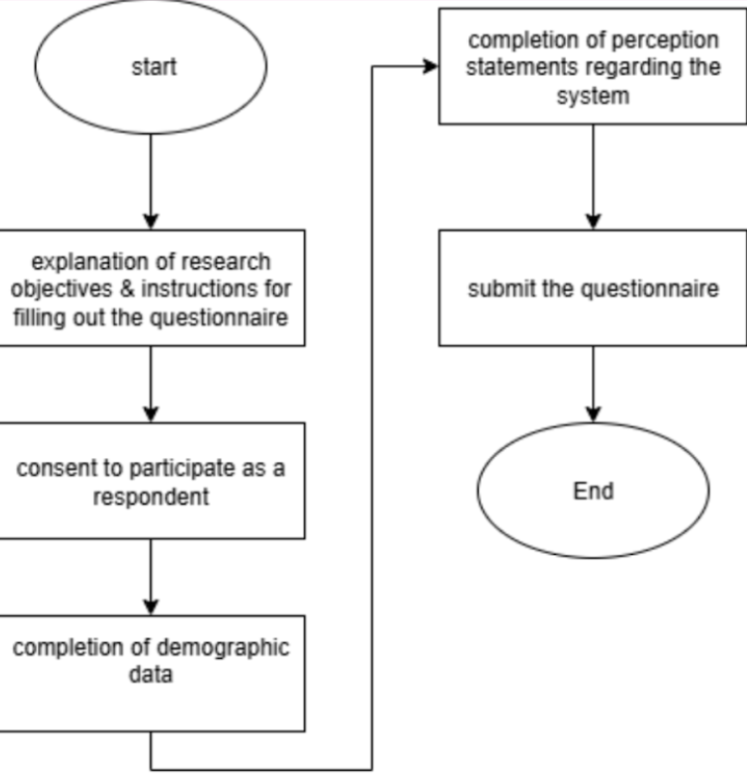
\includegraphics[width=0.7\textwidth]{Gambar/gambar7.2.png}
        \caption{Pengumpulan Data}
    \end{figure}

    Pada tahap penjelasan, peneliti menjelaskan cara mengisi kuesioner, termasuk pernyataan dan variabel yang terkandung di dalamnya. Kuesioner ini mencakup variabel yang mencerminkan persepsi responden terhadap sistem bimbingan belajar. Tahap berikutnya adalah persetujuan responden. Responden adalah guru sekolah dasar di Malang, dengan usia rata-rata 35 tahun, pengalaman kerja rata-rata 7 tahun, tingkat pendidikan tertinggi rata-rata sarjana (S1), dan sebagian besar di antaranya mengajar mata pelajaran matematika. Setelah itu, dilanjutkan dengan tahap pengisian pernyataan persepsi, diikuti dengan pengembalian kuesioner.Alasan mereka dipilih sebagai responden target dalam studi ini adalah karena mereka adalah guru matematika yang mengajar di sekolah dasar di Kota Malang.

\subsection{Model Penerimaan Teknologi (TAM)}

    Model Penerimaan Teknologi (TAM) adalah salah satu model teoritis yang dikembangkan untuk memahami dan memprediksi penerimaan teknologi oleh pengguna. Model ini pertama kali diperkenalkan oleh Fred D. Davis pada tahun 1986 sebagai adaptasi dari Teori Tindakan Berpikir (TRA) oleh Fishbein dan Ajzen.
    
    TAM menjelaskan bahwa dua faktor utama mempengaruhi penerimaan teknologi: Kegunaan yang Dirasakan (PU) dan Kemudahan Penggunaan yang Dirasakan (PEOU) [5]. Kegunaan yang Dirasakan merujuk pada sejauh mana seseorang percaya bahwa menggunakan sistem tertentu akan meningkatkan kinerjanya, sementara Kemudahan Penggunaan yang Dirasakan merujuk pada sejauh mana seseorang percaya bahwa menggunakan sistem tersebut akan bebas dari upaya yang signifikan.
    
    Model ini menekankan bahwa jika pengguna menganggap teknologi sebagai sesuatu yang berguna dan mudah digunakan, mereka lebih cenderung memiliki sikap positif terhadap penggunaannya, yang pada gilirannya akan mendorong niat dan keputusan mereka untuk menggunakan teknologi tersebut.

    \begin{figure}[H]
        \centering
        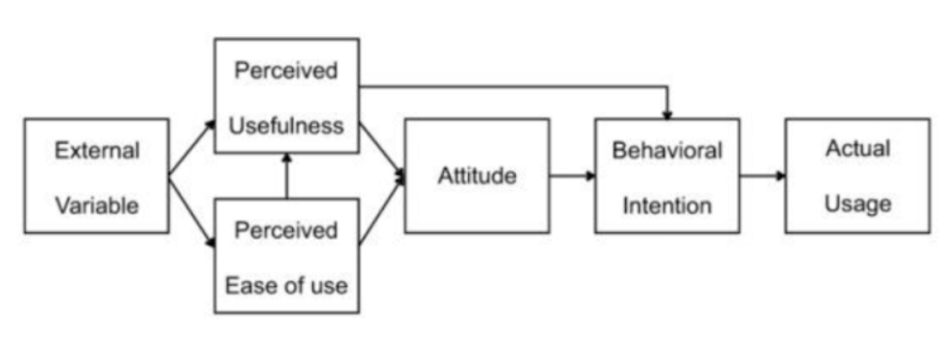
\includegraphics[width=0.7\textwidth]{Gambar/gambar7.3.png}
        \caption{Model Penerimaan Teknologi}
    \end{figure}

    Dalam Gambar 1, Model Penerimaan Teknologi (TAM) dapat diperluas melalui integrasi variabel eksternal, seperti dukungan organisasi, pelatihan, atau karakteristik individu, yang dapat mempengaruhi PU (Kegunaan yang Dirasakan) dan PEOU (Kemudahan Penggunaan yang Dirasakan) [6]. Hal ini membuat TAM relevan dalam berbagai konteks, termasuk bidang pendidikan.

    Di sisi lain, TAM banyak digunakan dalam konteks penelitian sistem informasi karena kesederhanaannya dan kemampuannya untuk menjelaskan niat perilaku terhadap penggunaan teknologi [6]. Dalam konteks pendidikan, model ini dapat digunakan untuk mengukur sejauh mana guru atau pendidik menerima dan bersedia menggunakan teknologi instruksional.

\subsection{Kontruksi TAM}

    Dalam adopsi teknologi baru di pendidikan, persepsi guru memainkan peran sentral. Oleh karena itu, untuk memahami faktor-faktor yang mempengaruhi penerimaan guru terhadap teknologi sistem penasihat, penelitian ini menggunakan pendekatan Model Penerimaan Teknologi (TAM) yang dikembangkan oleh Davis (1986) dan diperluas oleh Venkatesh dan Davis (2000).

    \begin{figure}[H]
        \centering
        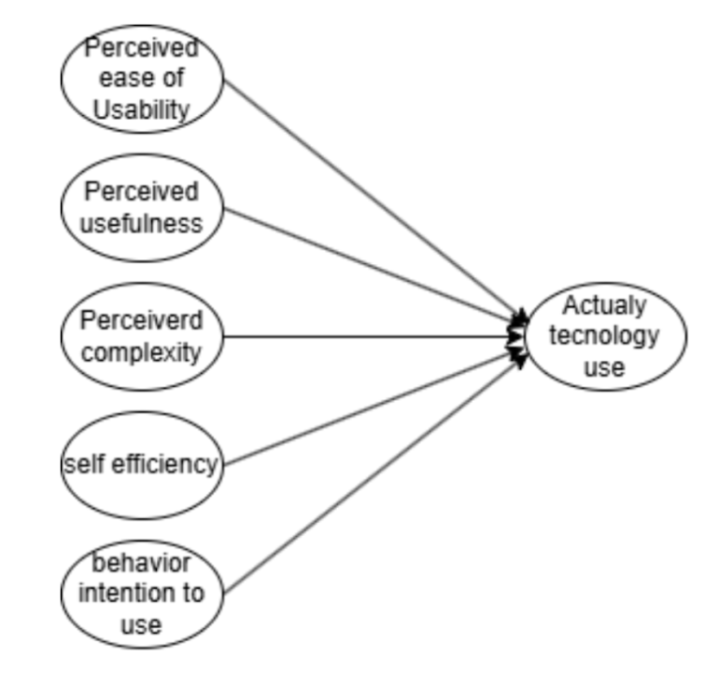
\includegraphics[width=0.7\textwidth]{Gambar/gambar7.4.png}
        \caption{Struktur Desain Penelitian Model}
    \end{figure}

    Model ini menjelaskan bahwa penerimaan teknologi dapat dipengaruhi oleh dua variabel utama: Kegunaan yang Dirasakan (PU) dan Kemudahan Penggunaan yang Dirasakan (PEOU). Selain itu, model ini juga dapat dikembangkan lebih lanjut dengan menambahkan variabel eksternal yang relevan dengan konteks penelitian, seperti Keyakinan Diri, Kompleksitas, Niat Perilaku untuk Menggunakan, dan Penggunaan Aktual. Model ini dapat dilihat pada Gambar 2.

    \begin{enumerate}
        \item Kemudahan Penggunaan yang Dirasakan
        
        Menjelaskan sejauh mana guru merasa bahwa sistem penasihat pembelajaran mudah dipelajari, dipahami, digunakan, dan diintegrasikan ke dalam aktivitas pengajaran.
        
        \item Kegunaan yang Dirasakan
        
        Menunjukkan keyakinan guru bahwa penggunaan sistem teknologi ini dapat meningkatkan efisiensi dan efektivitas dalam proses pengajaran dan pembelajaran, termasuk memberikan penilaian dan umpan balik kepada siswa.
        
        \item Kompleksitas yang Dirasakan
        
        Menilai tingkat kesulitan atau kompleksitas yang dirasakan oleh guru saat menggunakan sistem, baik dalam hal fitur, implementasi, maupun pemahaman terhadap hasil penilaian yang disediakan oleh sistem.
        
        \item Kepercayaan Diri
        
        Mengukur kepercayaan guru dalam mengoperasikan sistem, termasuk motivasi dan keterampilan mereka dalam menggunakan teknologi pendidikan dan memberikan umpan balik yang bermakna kepada siswa.
        
        \item Niat Perilaku untuk Menggunakan
        
        Menunjukkan sejauh mana guru memiliki niat atau keinginan untuk menggunakan sistem secara konsisten dalam kegiatan pengajaran, serta keterbukaan mereka untuk mengintegrasikan teknologi ke dalam proses pembelajaran.
        
        \item Penggunaan Teknologi yang Sebenarnya
        
        Mengacu pada tingkat penggunaan teknologi yang sebenarnya dalam aktivitas pembelajaran sehari-hari, termasuk sejauh mana guru menggunakan sistem untuk menilai, memantau, dan membimbing siswa.
    \end{enumerate}

\subsection{Analisis Data}

    Analisis data penelitian dilakukan menggunakan perangkat lunak IBM SPSS Statistics :

    \begin{enumerate}
        \item Uji Validitas
        
        Validitas berasal dari kata validitas, yang berarti sejauh mana alat ukur secara akurat dan tepat menjalankan fungsi pengukurannya [11]. Selain itu, validitas adalah ukuran yang menunjukkan apakah variabel yang diukur benar-benar mewakili variabel yang dimaksudkan untuk diteliti oleh peneliti [12].
        
        \item Uji Reliabilitas
        
        Keandalan adalah alat yang digunakan untuk mengukur kuesioner, yang berfungsi sebagai indikator variabel atau konstruk [13]. Sebuah kuesioner dikatakan andal atau dapat diandalkan jika respons seseorang terhadap pernyataan-pernyataan tersebut konsisten atau stabil dari waktu ke waktu. Keandalan suatu tes mengacu pada tingkat stabilitas, konsistensi, daya prediksi, dan akurasi.

        \item Analisis Data

        Analisis data adalah proses pencarian dan pengaturan data secara sistematis yang diperoleh dari wawancara, catatan lapangan, dan dokumentasi dengan mengelompokkan data ke dalam kategori, membaginya menjadi unit, mensintesisnya, mengaturnya ke dalam pola, memilih apa yang penting dan apa yang akan diteliti, serta menarik kesimpulan sehingga mudah dipahami oleh diri sendiri dan orang lain [10].

        \item Uji Normalitas

        Uji normalitas bertujuan untuk menentukan apakah residu atau variabel gangguan dalam model regresi mengikuti distribusi normal. Hal ini menunjukkan bahwa respons yang diberikan oleh responden dalam kuesioner akan bervariasi antara satu responden dengan responden lainnya. Oleh karena itu, uji normalitas dapat digunakan untuk menentukan apakah distribusi data pada pertanyaan tertentu memenuhi syarat normalitas. Uji normalitas sangat penting dalam statistik, terutama karena banyak metode analisis statistik mengasumsikan bahwa data yang digunakan berasal dari distribusi normal [14].

        \item Uji Multikolinearitas

        Multikolinearitas adalah fenomena dalam analisis regresi berganda yang terjadi ketika dua atau lebih variabel independen dalam model regresi memiliki hubungan linier yang sangat kuat. Hal ini menunjukkan adanya ketergantungan di antara variabel independen, yang dapat menyulitkan pemisahan efek individu masing-masing variabel terhadap variabel dependen. Keberadaan multikolinearitas dapat menyebabkan estimasi koefisien regresi yang tidak stabil dan tidak dapat diandalkan, serta meningkatkan varians koefisien regresi, yang dapat menyebabkan kesalahan saat menafsirkan hasil analisis [15].

        \item Uji Heteroskedastisitas

        Heteroskedastisitas adalah masalah yang terjadi dalam model regresi linier ketika varians kesalahan (residu) tidak konstan di seluruh nilai variabel independen. Dalam kehadiran heteroskedastisitas, varians residu cenderung berubah seiring dengan perubahan nilai variabel independen. Herbert Glejser mengembangkan uji baru untuk mendeteksi heteroskedastisitas. Uji ini melibatkan regresi nilai absolut residual dari model regresi asli terhadap variabel independen yang diduga terkait dengan varians residual. Jika koefisien regresi secara statistik signifikan, hal ini menunjukkan adanya heteroskedastisitas [16].

        \item Uji t

        Uji t adalah metode statistik yang digunakan untuk menentukan apakah ada perbedaan yang signifikan antara rata-rata dua kelompok data. Teknik ini sering digunakan dalam penelitian kuantitatif, terutama ketika peneliti ingin mengevaluasi efek atau perbedaan perlakuan antara dua kelompok yang dianalisis [17].

        \item Uji F

        Uji F dilakukan dengan membandingkan nilai F yang dihitung dari hasil regresi dengan nilai F tabel berdasarkan derajat kebebasan tertentu dan tingkat signifikansi yang telah ditentukan (biasanya 5\% atau 0,05) [18]. Jika nilai F yang dihitung lebih besar dari nilai F tabel, dapat disimpulkan bahwa semua variabel independen dalam model secara bersamaan memiliki efek signifikan terhadap variabel dependen.
    \end{enumerate}

\section{Hasil dan Pembahasan}

    Data dalam penelitian ini berasal dari skor kuesioner mengenai persepsi guru sekolah dasar di Malang terkait penggunaan sistem penasihat pembelajaran dalam konteks kelas. Penelitian ini dilakukan dengan pendekatan kuantitatif deskriptif melalui penyebaran kuesioner sebagai instrumen utama. Kuesioner yang terdiri dari 25 pertanyaan dibagikan kepada guru, dan wawancara juga dilakukan dengan guru yang mengajar di sekolah dasar. Jumlah responden dalam penelitian ini adalah 20 guru sekolah dasar.

\subsection{Uji Validitas}

    Uji validitas juga dilakukan menggunakan perangkat lunak IBM SPSS untuk mengukur hubungan antara skor setiap item dan skor total variabel pada instrumen penelitian. Tabel hasil uji validitas dapat dilihat pada tabel di bawah ini.

    \begin{table}[H]
        \centering
        \caption{Hasil Uji Validitas pada Variabel Kemudahan Penggunaan yang Dirasakan}
        \label{tab:uji-validitas-kemudahan}
        \begin{tabularx}{\textwidth}{p{4.5cm}lXXXl}
            \toprule
            \textbf{Variabel} & \textbf{Kode Item} & \textbf{Nilai Korelasi yang Dihitung} & \textbf{Nilai r-tabel} & \textbf{Sig.} & \textbf{Deskripsi} \\
            \midrule
            \multirow{4}{=}{Kemudahan Penggunaan yang Dirasakan}
                & X1.1 & 0.721 & 0.444 & 0.000 & Valid \\
                & X1.2 & 0.663 & 0.444 & 0.001 & Valid \\
                & X1.3 & 0.838 & 0.444 & 0.000 & Valid \\
                & X1.4 & 0.765 & 0.444 & 0.000 & Valid \\
            \bottomrule
        \end{tabularx}
    \end{table}

    Dalam Tabel 1, variabel diukur menggunakan empat item pernyataan (X1.1 hingga X1.4) yang bertujuan untuk menilai persepsi guru terhadap kemudahan pemahaman dan penggunaan sistem penasihat pembelajaran. Hasil uji menunjukkan bahwa semua item memiliki nilai korelasi di atas r-table (0.444) dan nilai signifikansi yang sangat rendah (p<0.01). Nilai korelasi berkisar antara 0.663 hingga 0.838, menunjukkan hubungan yang kuat dan signifikan antara setiap item dan skor total variabel.

    \begin{table}[H]
        \centering
        \caption{Hasil Uji Validitas pada Persepsi Kegunaan}
        \label{tab:uji-validitas-kegunaan}
        \begin{tabularx}{\textwidth}{p{4.5cm}lXXXl}
            \toprule
            \textbf{Variabel} & \textbf{Kode Item} & \textbf{Nilai Korelasi yang Dihitung} & \textbf{Nilai r-tabel} & \textbf{Sig.} & \textbf{Deskripsi} \\
            \midrule
            \multirow{5}{=}{Kegunaan yang Dirasakan}
                & X2.1 & 0.777 & 0.444 & 0.000 & Valid \\
                & X2.2 & 0.719 & 0.444 & 0.000 & Valid \\
                & X2.3 & 0.798 & 0.444 & 0.000 & Valid \\
                & X2.4 & 0.781 & 0.444 & 0.000 & Valid \\
                & X2.5 & 0.706 & 0.444 & 0.001 & Valid \\
            \bottomrule
        \end{tabularx}
    \end{table}

    Dalam Tabel 2, variabel diukur menggunakan lima item pernyataan (X2.1 hingga X2.5) yang dirancang untuk menangkap persepsi guru mengenai manfaat sistem dalam meningkatkan efektivitas pengajaran. Hasil analisis data menunjukkan bahwa semua item memiliki nilai r antara 0.706 dan 0.798, dengan signifikansi $\leq 0.001$, menunjukkan hubungan yang kuat dan signifikan.

    \begin{table}[H]     \centering
        \caption{Hasil Uji Validitas pada Kompleksitas}
        \label{tab:uji-validitas-kompleksitas}
        \begin{tabularx}{\textwidth}{p{4.5cm}lXXXl}
            \toprule
            \textbf{Variabel} & \textbf{Kode Item} & \textbf{Nilai Korelasi yang Dihitung} & \textbf{Nilai r-tabel} & \textbf{Sig.} & \textbf{Deskripsi} \\
            \midrule
            \multirow{3}{=}{Kompleksitas}
                & X3.1 & 0.869 & 0.444 & 0.000 & Valid \\
                & X3.2 & 0.865 & 0.444 & 0.000 & Valid \\
                & X3.3 & 0.617 & 0.444 & 0.004 & Valid \\
            \bottomrule
        \end{tabularx}
    \end{table}

    Dalam Tabel 3, variabel ini terdiri dari tiga item (X3.1 hingga X3.3) yang mengukur persepsi guru terhadap kompleksitas sistem. Meskipun konsepnya negatif, hasil korelasi menunjukkan bahwa semua item memiliki nilai r yang dihitung berkisar antara 0.617 hingga 0.869, menunjukkan korelasi yang kuat dan signifikan dengan skor total. Temuan ini mengonfirmasi bahwa item-item variabel dalam Kompleksitas secara efektif mengukur persepsi guru terhadap tantangan teknis atau kesulitan dalam menggunakan sistem. Nilai tertinggi, X3.1 (r = 0.869), menyoroti bahwa guru memberikan penekanan yang signifikan pada aspek teknis.

    \begin{table}[H]
        \centering
        \caption{Hasil Uji Validitas pada Self-Efficacy (Efektivitas Diri)}
        \label{tab:uji-validitas-self-efficacy}
        \begin{tabularx}{\textwidth}{p{4.5cm}lXXXl}
            \toprule
            \textbf{Variabel} & \textbf{Kode Item} & \textbf{Nilai Korelasi yang Dihitung} & \textbf{Nilai r-tabel} & \textbf{Sig.} & \textbf{Deskripsi} \\
            \midrule
            \multirow{5}{=}{Efektivitas Diri}
                & X4.1 & 0.811 & 0.444 & 0.000 & Valid \\
                & X4.2 & 0.782 & 0.444 & 0.000 & Valid \\
                & X4.3 & 0.658 & 0.444 & 0.002 & Valid \\
                & X4.4 & 0.651 & 0.444 & 0.002 & Valid \\
                & X4.5 & 0.452 & 0.444 & 0.045 & Valid \\
            \bottomrule
        \end{tabularx}
    \end{table}

    Dalam Tabel 4, variabel Self-Efficacy mencerminkan keyakinan guru dalam menggunakan sistem dan diukur melalui lima item (X4.1 hingga X4.5). Hasil uji validitas menunjukkan bahwa semua item valid, dengan nilai r berkisar antara 0.452 hingga 0.811, dan semua nilai signifikansi < 0.05. Meskipun satu item (X4.5) memiliki nilai korelasi mendekati ambang batas minimum (r = 0.452), nilainya tetap berada dalam rentang statistik yang dapat diterima. Hasil ini menunjukkan bahwa guru memiliki persepsi yang relatif konsisten tentang kemampuan mereka dalam mengoperasikan sistem pembelajaran, dan semua item instrumen valid dalam mengukur Self-Efficacy ini.

    \begin{table}[H]
        \centering
        \caption{Hasil Uji Validitas pada Niat Perilaku untuk Menggunakan}
        \label{tab:uji-validitas-niat-perilaku}
        \begin{tabularx}{\textwidth}{p{5cm}lXXXl}
            \toprule
            \textbf{Variabel} & \textbf{Kode Item} & \textbf{Nilai Korelasi yang Dihitung} & \textbf{Nilai r-tabel} & \textbf{Sig.} & \textbf{Deskripsi} \\
            \midrule
            \multirow{4}{=}{Niat Perilaku untuk Menggunakan}
                & X5.1 & 0.774 & 0.444 & 0.000 & Valid \\
                & X5.2 & 0.645 & 0.444 & 0.002 & Valid \\
                & X5.3 & 0.591 & 0.444 & 0.006 & Valid \\
                & X5.4 & 0.866 & 0.444 & 0.002 & Valid \\
            \bottomrule
        \end{tabularx}
    \end{table}

    Dalam Tabel 5, variabel ini mengukur niat dan kesediaan guru untuk menggunakan sistem secara berkelanjutan, yang dievaluasi melalui empat item pernyataan (X5.1 hingga X5.4). Hasil analisis menunjukkan bahwa semua item memiliki korelasi yang kuat dan signifikan dengan skor total, dengan nilai r berkisar antara 0.591 hingga 0.866. Nilai signifikansi untuk semua item berada di bawah 0.05, dengan sebagian besar di bawah 0.01, menunjukkan kekuatan pengukuran yang sangat baik. Hal ini menunjukkan bahwa guru menunjukkan tingkat konsistensi yang tinggi dalam respons mereka terkait niat untuk terus menggunakan sistem.

    \begin{table}[H]
        \centering
        \caption{Hasil Uji Validitas pada Penggunaan Teknologi Aktual}
        \label{tab:uji-validitas-penggunaan-teknologi}
        \begin{tabularx}{\textwidth}{p{5cm}lXXXl}
            \toprule
            \textbf{Variabel} & \textbf{Kode Item} & \textbf{Nilai Korelasi yang Dihitung} & \textbf{Nilai r-tabel} & \textbf{Sig.} & \textbf{Deskripsi} \\
            \midrule
            \multirow{4}{=}{Penggunaan Teknologi Aktual}
                & Y1.1 & 0.626 & 0.444 & 0.003 & Valid \\
                & Y1.2 & 0.830 & 0.444 & 0.000 & Valid \\
                & Y1.3 & 0.745 & 0.444 & 0.000 & Valid \\
                & Y1.4 & 0.626 & 0.444 & 0.003 & Valid \\
            \bottomrule
        \end{tabularx}
    \end{table}

    Dalam Tabel 6, variabel Penggunaan Teknologi Aktual mengukur sejauh mana guru menggunakan sistem penasihat pembelajaran dalam praktik pengajaran sehari-hari mereka. Variabel ini dievaluasi melalui empat item pernyataan (Y1 hingga Y4). Hasil uji validitas menggunakan korelasi Pearson menunjukkan bahwa tiga dari empat item memiliki nilai r lebih besar dari 0,444 dan nilai signifikansi kurang dari 0,05, menunjukkan validitas. Meskipun korelasi antara beberapa item dalam indikator yang sama bervariasi, hubungan antara setiap item dan skor total variabel Penggunaan Teknologi Aktual menunjukkan kekuatan korelasi yang tinggi dan signifikan. Semua item memiliki nilai korelasi jauh di atas ambang batas minimum 0.444 dan nilai signifikansi yang sangat rendah, menunjukkan bahwa setiap pernyataan dalam konstruksi Penggunaan Teknologi Aktual memenuhi kriteria validitas.


\subsection{Uji Reliabilitas}

    Uji reliabilitas dilakukan menggunakan metode Cronbach’s Alpha. Tujuan uji reliabilitas adalah untuk menentukan sejauh mana instrumen konsisten dan stabil dalam mengukur suatu konstruk. Uji reliabilitas dilakukan dengan bantuan perangkat lunak IBM SPSS untuk menilai konsistensi setiap item pada instrumen penelitian.

    \begin{table}[H]
        \centering
        \caption{Hasil Uji Reliabilitas Persepsi Guru Sekolah Dasar di Malang}
        \label{tab:uji-reliabilitas-guru}
        \begin{tabularx}{\textwidth}{p{6cm}ccl}
            \toprule
            \textbf{Variabel} & \textbf{Jumlah Item} & \textbf{Cronbach’s Alpha} & \textbf{Kesimpulan} \\
            \midrule
            Kemudahan Penggunaan yang Dirasakan & 4 & 0.724 & Terpercaya (Baik) \\
            Kegunaan yang Dirasakan              & 5 & 0.807 & Terpercaya (Baik) \\
            Kompleksitas                         & 3 & 0.701 & Terpercaya (Baik) \\
            Kepercayaan Diri                     & 5 & 0.730 & Terpercaya (Baik) \\
            Niat Perilaku untuk Menggunakan      & 4 & 0.679 & Terpercaya (Baik) \\
            Penggunaan Teknologi yang Sebenarnya & 4 & 0.626 & Terpercaya (Baik) \\
            \bottomrule
        \end{tabularx}
    \end{table}

    Dalam Tabel 7, hasil uji menunjukkan bahwa semua variabel dalam studi ini memiliki nilai Cronbach’s Alpha lebih dari 0,60, menunjukkan bahwa instrumen yang digunakan dapat diandalkan dan sesuai untuk analisis lebih lanjut.
    
\subsection{Analisis Data}

    \begin{table}[H]
        \centering
        \caption{Hasil Analisis Data Persepsi Guru Sekolah Dasar di Malang}
        \label{tab:analisis-data-guru}
        \begin{tabularx}{\textwidth}{p{6cm}ccccc}
            \toprule
            \textbf{Variabel} & \textbf{N} & \textbf{Min} & \textbf{Maks} & \textbf{Rata-rata} & \textbf{Simpangan Baku} \\
            \midrule
            Kemudahan Penggunaan yang Dirasakan & 20 & 10 & 16 & 12.50 & 1.469 \\
            Kegunaan yang Dirasakan              & 20 & 11 & 19 & 15.30 & 2.029 \\
            Kompleksitas                         & 20 & 4  & 8  & 6.00  & 1.451 \\
            Kepercayaan Diri                     & 20 & 9  & 15 & 12.60 & 1.353 \\
            Niat Perilaku untuk Menggunakan      & 20 & 9  & 15 & 12.40 & 1.501 \\
            Penggunaan Teknologi yang Sebenarnya & 20 & 10 & 15 & 12.00 & 1.376 \\
            \bottomrule
        \end{tabularx}
    \end{table}

    Berdasarkan analisis deskriptif pada Tabel 8, dapat dilihat bahwa secara umum, guru memiliki pandangan positif terhadap sistem penasihat pembelajaran digital. Skor rata-rata untuk Kemudahan Penggunaan yang Dirasakan adalah 12,50, menunjukkan bahwa guru merasa sistem tersebut cukup mudah digunakan. Skor tertinggi terdapat pada Kegunaan yang Dirasakan, dengan rata-rata 15,30, artinya guru menganggap sistem tersebut sangat bermanfaat. Sementara itu, Kompleksitas memiliki skor rata-rata 6,00, menunjukkan bahwa sistem terasa agak kompleks tetapi masih dapat dikelola. Skor rata-rata untuk Kepercayaan Diri adalah 12,60, menunjukkan bahwa guru merasa percaya diri dalam menggunakan sistem. Niat Perilaku untuk Menggunakan memiliki skor rata-rata 12,40, menunjukkan bahwa guru berniat untuk terus menggunakan sistem. Akhirnya, Penggunaan Teknologi Aktual memiliki skor rata-rata 12,00, yang menunjukkan bahwa guru telah menggunakan sistem tersebut secara sering. Secara keseluruhan, data menunjukkan bahwa guru menerima sistem tersebut dengan baik dan mendukung penggunaannya dalam proses pembelajaran.

\subsection{Uji Normalitas}

    \begin{table}[H]
        \centering
        \caption{Hasil Uji Normalitas Persepsi Guru Sekolah Dasar di Malang}
        \label{tab:uji-normalitas-guru}
        \begin{tabularx}{0.8\textwidth}{p{7cm}r}
            \toprule
            \textbf{Statistik} & \textbf{Nilai} \\
            \midrule
            N & 20 \\
            Rata-rata & 0.0000000 \\
            Simpangan baku & 0.74985014 \\
            Perbedaan Ekstrem Terbesar (Absolut) & 0.106 \\
            Perbedaan Ekstrem Terbesar (Positif) & 0.106 \\
            Perbedaan Ekstrem Terbesar (Negatif) & -0.084 \\
            Kolmogorov-Smirnov Z & 0.106 \\
            Signifikansi Asimtotik (dua ekor) & 0.200 \\
            \bottomrule
        \end{tabularx}
    \end{table}

    Berdasarkan Tabel 9, hasil uji menunjukkan bahwa nilai Asymp. Sig. adalah 0.200, yang lebih besar dari 0.05. Hal ini menunjukkan bahwa data residu dalam model regresi mengikuti distribusi normal. Oleh karena itu, salah satu persyaratan asumsi klasik dalam regresi linier, yaitu asumsi normalitas residu, telah terpenuhi. Selain itu, nilai perbedaan absolut ekstrem terbesar sebesar 0,106 menunjukkan bahwa tidak ada penyimpangan yang signifikan antara distribusi data residu dan distribusi normal teoretis. Berdasarkan hasil uji, nilai Asymp. Sig. sebesar 0,200, yang lebih besar dari 0,05. Hal ini menunjukkan bahwa data residu dalam model regresi mengikuti distribusi normal. Oleh karena itu, salah satu persyaratan asumsi klasik dalam regresi linier, yaitu asumsi normalitas residu, telah terpenuhi. Selain itu, nilai perbedaan absolut ekstrem sebesar 0,106 menunjukkan bahwa tidak ada penyimpangan yang signifikan antara distribusi data residu dan distribusi normal teoretis.

\subsection{Uji Multikolinearitas}

    \begin{table}[H]
        \centering
        \caption{Hasil Uji Multikolinearitas Persepsi Guru Sekolah Dasar di Malang}
        \label{tab:uji-multikolinearitas-guru}
        \begin{tabularx}{0.8\textwidth}{p{7cm}r}
            \toprule
            \textbf{Statistik} & \textbf{Nilai} \\
            \midrule
            N & 20 \\
            Rata-rata & 0.0000000 \\
            Simpangan baku & 0.74985014 \\
            Perbedaan Ekstrem Terbesar (Absolut) & 0.106 \\
            Perbedaan Ekstrem Terbesar (Positif) & 0.106 \\
            Perbedaan Ekstrem Terbesar (Negatif) & -0.084 \\
            Kolmogorov-Smirnov Z & 0.106 \\
            Signifikansi Asimtotik (dua ekor) & 0.200 \\
            \bottomrule
        \end{tabularx}
    \end{table}

    Berdasarkan Tabel 10, hasil uji multikolinearitas di atas menunjukkan bahwa semua variabel independen memiliki nilai Toleransi > 0,10 dan nilai VIF < 10. Nilai VIF tertinggi ditemukan pada variabel Niat Perilaku, yaitu 3.964, namun nilai ini masih jauh di bawah ambang batas kritis 10. Demikian pula, nilai Toleransi untuk semua variabel berada di atas 0.10, menunjukkan bahwa tidak ada indikasi serius multikolinearitas dalam model regresi. 

\subsection{Uji Heteroskedastisitas}

    \begin{table}[H]
        \centering
        \caption{Hasil Uji Heteroskedastisitas Persepsi Guru Sekolah Dasar di Malang}
        \label{tab:uji-heteroskedastisitas}
        \begin{tabularx}{\textwidth}{lcccc}
            \toprule
            \textbf{Variabel Independen} & \textbf{B} & \textbf{Std. Error} & \textbf{t} & \textbf{Sig.} \\
            \midrule
            (Konstanta) & -3.166 & 0.968 & -3.286 & 0.006 \\
            Kemudahan Penggunaan yang Dirasakan & 0.081 & 0.091 & 0.885 & 0.391 \\
            Persepsi Kegunaan & 0.107 & 0.066 & 1.623 & 0.127 \\
            Kompleksitas & 0.063 & 0.058 & 1.076 & 0.300 \\
            Kepercayaan Diri & 0.146 & 0.106 & 1.374 & 0.191 \\
            Niat Perilaku & -0.089 & 0.097 & -0.922 & 0.372 \\
            \bottomrule
        \end{tabularx}
    \end{table}

    Berdasarkan Tabel 11, hasil uji heteroskedastisitas menggunakan metode Glejser menunjukkan bahwa semua variabel independen memiliki nilai signifikansi lebih besar dari 0.05. Oleh karena itu, tidak ada variabel prediktor yang secara signifikan mempengaruhi nilai absolut residu. Berdasarkan hasil uji heteroskedastisitas menggunakan metode Glejser, semua variabel independen memiliki nilai signifikansi lebih besar dari 0.05. Oleh karena itu, tidak ada variabel prediktor yang secara signifikan mempengaruhi nilai absolut residu. Berdasarkan hasil uji heteroskedastisitas menggunakan metode Glejser, semua variabel independen memiliki nilai signifikansi lebih besar dari 0,05. Oleh karena itu, tidak ada variabel prediktor yang secara signifikan mempengaruhi nilai absolut residu.

\subsection{Uji t}

    \begin{table}[H]
        \centering
        \caption{Hasil Uji t Persepsi Guru Sekolah Dasar di Malang}
        \label{tab:uji-t}
        \begin{tabularx}{\textwidth}{lccccc}
            \toprule
            \textbf{Variabel Independen} & \textbf{B} & \textbf{Kesalahan Standar} & \textbf{Beta} & \textbf{t} & \textbf{Sig.} \\
            \midrule
            Konstanta & 7.330 & 2.659 & - & 2.757 & 0.015 \\
            Kemudahan Penggunaan yang Dirasakan & 0.199 & 0.251 & 0.212 & 0.792 & 0.442 \\
            Kegunaan yang Dirasakan & -0.288 & 0.181 & -0.425 & -1.594 & 0.133 \\
            Kompleksitas & -0.367 & 0.160 & -0.387 & -2.301 & 0.037 \\
            Keyakinan Diri & 0.207 & 0.291 & 0.203 & 0.711 & 0.489 \\
            Niat Perilaku & 0.499 & 0.266 & 0.544 & 1.878 & 0.081 \\
            \bottomrule
        \end{tabularx}
    \end{table}

    Berdasarkan hasil uji t parsial pada Tabel 12, hanya variabel Kompleksitas yang ditemukan memiliki pengaruh signifikan terhadap Penggunaan Teknologi Aktual, dengan nilai signifikansi (p) sebesar 0,037 < 0,05. Hal ini menunjukkan bahwa semakin kompleks sistem yang dirasakan oleh guru, semakin rendah kecenderungan mereka untuk benar-benar menggunakannya. Variabel lain seperti Kemudahan Penggunaan yang Dirasakan, Kegunaan yang Dirasakan, Keyakinan Diri, dan Niat Perilaku untuk Menggunakan tidak menunjukkan efek yang signifikan secara statistik, meskipun niat untuk menggunakan mendekati ambang batas signifikansi, menunjukkan potensi pengaruh yang memerlukan penyelidikan lebih lanjut dengan ukuran sampel yang lebih besar.

\subsection{Uji f}

    \begin{table}[H]
        \centering
        \caption{Hasil Uji F Persepsi Guru Sekolah Dasar di Malang}
        \label{tab:uji-f}
        \begin{tabularx}{\textwidth}{lccccc}
            \toprule
            \textbf{Sumber Variasi} & \textbf{Jumlah Kuadrat} & \textbf{df} & \textbf{Rata-rata Kuadrat} & \textbf{F} & \textbf{Sig.} \\
            \midrule
            Regresi & 25,317 & 5 & 5,063 & 6,635 & 0,002 \\
            Sisa & 10,683 & 14 & 0,763 & - & - \\
            Total & 36,000 & 19 & - & - & - \\
            \bottomrule
        \end{tabularx}
    \end{table}

    Berdasarkan hasil uji F pada Tabel 13, nilai F yang dihitung adalah 6,635 dengan tingkat signifikansi (p = 0,002). Nilai p sebesar 0,002 menunjukkan bahwa probabilitas terjadinya hasil ini secara kebetulan sangat kecil jika semua koefisien sebenarnya tidak memiliki pengaruh. Selain itu, nilai ini jauh lebih kecil daripada tingkat signifikansi 0,05, yang berarti model regresi secara keseluruhan secara statistik signifikan. Temuan ini mengonfirmasi bahwa persepsi guru terhadap berbagai atribut sistem secara signifikan berkontribusi dalam menjelaskan penggunaan sistem penasihat pembelajaran berbasis teknologi. Hasil ini juga memperkuat validitas model regresi yang digunakan, memberikan dasar statistik yang kokoh bahwa semua konstruk dalam kerangka kerja berperan dalam membentuk sikap dan perilaku guru terhadap penggunaan teknologi dalam pendidikan.

\section{Kesimpulan}

    Berdasarkan hasil analisis data dan pembahasan, penelitian ini menyimpulkan bahwa guru sekolah dasar di Kota Malang secara umum memiliki persepsi positif terhadap sistem penasihat pembelajaran digital dan terbuka terhadap implementasinya dalam kegiatan pembelajaran di kelas. Hal ini didukung oleh analisis deskriptif, yang menunjukkan nilai rata-rata yang relatif tinggi pada variabel utama TAM, seperti Kegunaan yang Dirasakan (rata-rata = 15,30) dan Kepercayaan Diri (rata-rata = 12,60), menunjukkan bahwa guru menganggap sistem ini bermanfaat dan merasa percaya diri dalam menggunakannya. Berdasarkan hasil uji t parsial (Tabel 12), dari lima variabel independen, hanya Kompleksitas yang memiliki pengaruh signifikan terhadap Penggunaan Teknologi Aktual (p = 0,037) dengan koefisien negatif (B = –0,367), artinya semakin kompleks sistem tersebut dipersepsikan oleh guru, semakin kecil kemungkinan mereka untuk menggunakannya. Variabel lain seperti Kemudahan Penggunaan yang Dirasakan (p = 0,442), Kegunaan yang Dirasakan (p = 0,133), Keyakinan Diri (p = 0,489), dan Niat Perilaku untuk Menggunakan (p = 0,081) tidak menunjukkan efek yang signifikan secara statistik, meskipun niat menunjukkan kecenderungan mendekati signifikansi. Selain itu, hasil uji F (Tabel 13) menunjukkan bahwa model regresi secara keseluruhan secara statistik signifikan, dengan nilai F sebesar 6.635 dan tingkat signifikansi p = 0.002. Ini berarti semua variabel independen secara kolektif memiliki pengaruh signifikan terhadap Penggunaan Teknologi Aktual. Hasil ini memperkuat validitas model regresi dan menunjukkan bahwa variabel yang diukur berkontribusi dalam menjelaskan perilaku guru dalam mengadopsi teknologi. Kesimpulannya, meskipun tidak semua variabel secara individu menunjukkan pengaruh yang signifikan, kombinasi persepsi guru tentang kemudahan penggunaan, kegunaan, dan kepercayaan diri memainkan peran penting dalam mendorong penggunaan sistem yang sebenarnya. Temuan ini menyoroti pentingnya mengurangi kompleksitas sistem dan menyediakan pelatihan yang memadai untuk mendukung adopsi teknologi yang lebih luas. Studi ini memberikan landasan yang kuat untuk mengembangkan kebijakan pendidikan berbasis teknologi yang selaras dengan penerimaan guru dan realitas pembelajaran di kelas sekolah dasar Indonesia.
\chapter{KESIMPULAN DAN SARAN}

Kami telah melakukan eksperimen awal dalam memvisualisasikan karakteristik siswa. Meskipun peta yang dihasilkan intuitif dan dalam beberapa hal informatif untuk memahami karakteristik siswa, peta tersebut hanya memberikan gambaran sekilas untuk satu tes tertentu. Dalam penelitian kami selanjutnya, kami berencana mengintegrasikan informasi dari peta ini ke dalam grafik kesamaan yang lebih baik menggambarkan kesamaan siswa secara hierarkis. Kami kemudian akan menggunakan grafik-grafik ini untuk secara otomatis menghasilkan saran pembelajaran yang dapat disesuaikan secara manual oleh guru dengan tujuan utama membantu siswa.
SOM-m-AT diusulkan sebagai metode baru untuk mempelajari kesamaan siswa dalam sistem bimbingan. Melalui beberapa eksperimen empiris, dapat diamati bahwa metode SOM-m-AT yang diusulkan outperforms SOM dalam efisiensi pembelajaran dan tingkat keberhasilan. Dalam penelitian ini, dengan metode SOM m-AT yang diusulkan, kami menemukan siswa dengan performa terburuk. Kita dapat mengetahui masalah yang dihadapi siswa, sehingga: menemukan siswa terdekat untuk mencoba menyelesaikan masalah yang terkait dengan strategi berpikir. Penelitian ini dapat memberikan informasi kepada guru untuk memberikan umpan balik yang sesuai berdasarkan masalah yang dihadapi siswa.


Berdasarkan hasil analisis data dan pembahasan, penelitian ini menyimpulkan bahwa guru sekolah dasar di Kota Malang secara umum memiliki persepsi positif terhadap sistem penasihat pembelajaran digital dan terbuka terhadap implementasinya dalam kegiatan pembelajaran di kelas. Hal ini didukung oleh analisis deskriptif, yang menunjukkan nilai rata-rata yang relatif tinggi pada variabel utama TAM, seperti Kegunaan yang Dirasakan (rata-rata = $15,30$) dan Kepercayaan Diri (rata-rata = $12,60$), menunjukkan bahwa guru menganggap sistem ini bermanfaat dan merasa percaya diri dalam menggunakannya. Berdasarkan hasil uji t parsial (Tabel 12), dari lima variabel independen, hanya Kompleksitas yang memiliki pengaruh signifikan terhadap Penggunaan Teknologi Aktual ($p = 0,037$) dengan koefisien negatif ($B = –0,367$), artinya semakin kompleks sistem tersebut dipersepsikan oleh guru, semakin kecil kemungkinan mereka untuk menggunakannya. Variabel lain seperti Kemudahan Penggunaan yang Dirasakan ($p = 0,442$), Kegunaan yang Dirasakan ($p = 0,133$), Keyakinan Diri ($p = 0,489$), dan Niat Perilaku untuk Menggunakan ($p = 0,081$) tidak menunjukkan efek yang signifikan secara statistik, meskipun niat menunjukkan kecenderungan mendekati signifikansi. Selain itu, hasil uji F (Tabel 13) menunjukkan bahwa model regresi secara keseluruhan secara statistik signifikan, dengan nilai F sebesar 6.635 dan tingkat signifikansi $p = 0.002$. Ini berarti semua variabel independen secara kolektif memiliki pengaruh signifikan terhadap Penggunaan Teknologi Aktual. Hasil ini memperkuat validitas model regresi dan menunjukkan bahwa variabel yang diukur berkontribusi dalam menjelaskan perilaku guru dalam mengadopsi teknologi. Kesimpulannya, meskipun tidak semua variabel secara individu menunjukkan pengaruh yang signifikan, kombinasi persepsi guru tentang kemudahan penggunaan, kegunaan, dan kepercayaan diri memainkan peran penting dalam mendorong penggunaan sistem yang sebenarnya. Temuan ini menyoroti pentingnya mengurangi kompleksitas sistem dan menyediakan pelatihan yang memadai untuk mendukung adopsi teknologi yang lebih luas. Studi ini memberikan landasan yang kuat untuk mengembangkan kebijakan pendidikan berbasis teknologi yang selaras dengan penerimaan guru dan realitas pembelajaran di kelas sekolah dasar Indonesia.


\nocite{*}

\DaftarPustaka{pustaka}
\BukaLampiran
\lampiran

\end{document}
